\documentclass[ a4paper,
                oneside,
                toc=bibliography,
                toc=listof
                ]{scrbook}

\usepackage[ngerman]{babel} % If the thesis is in English
\usepackage[hidelinks]{hyperref}
\usepackage[table]{xcolor}
\usepackage {longtable}
\usepackage{tikz}
\usetikzlibrary{positioning,calc}
\usepackage{tikz-uml}
\usetikzlibrary{positioning, arrows.meta}
\usepackage{geometry}
\usetikzlibrary{matrix}
\usetikzlibrary{fit,matrix,shapes.geometric}
\usetikzlibrary{positioning, shapes, arrows, decorations.pathreplacing}

\usepackage{nicematrix,booktabs,tikz}
\usepackage{harveyballs}
\usepackage{tabularx}
\usepackage{pgfgantt}
\usepackage{pgf-umlsd}
\usepackage[T1]{fontenc}
\usepackage[utf8]{inputenc}
\usepackage{amsmath}
\usepackage[nohyperlinks, printonlyused]{acronym}
\usepackage{listings}
%\usepackage{xcolor}
\usepackage{amssymb}
\usepackage{forest}

\lstset{
	language=[Sharp]C,
	basicstyle=\ttfamily,
	keywordstyle=\color{blue},
	commentstyle=\color{green!40!black},
	stringstyle=\color{orange},
	showstringspaces=false,
	breaklines=true,
	breakatwhitespace=true,
	tabsize=1,
	frame=single,
	gobble=2,     % Entfernt 4 Leerzeichen am Anfang jeder Zeile
	literate=%
		{Ö}{{\"O}}1
		{Ä}{{\"A}}1
		{Ü}{{\"U}}1
		{ß}{{\ss}}1
		{ü}{{\"u}}1
		{ä}{{\"a}}1
		{ö}{{\"o}}1
}

%\usepackage[english, ngerman]{babel} % If the thesis is in German


% This class does the ISW styling for you (together with scrbook).
%
% It handles the following:
% - Proper input and font encoding (Just type, don't care about the LaTeX compiler you use or how to type German umlauts)
% - Fonts with ligatures and kerning (Tex Gyre fonts are used, part of every LaTeX installation, text is nice to read)
% - Bibliography styling for biblatex (declare your bibliography file and you are ready to go)
% - Provide command for title page (\makeISWtitle) and declaration of originality ( \declarationOfOriginality)
% - Loads packages "biblatex" and "graphics"
\usepackage[
    type=study, % master, bachelor, bachelorproject
]{iswthesis}

%Path to .bib-File(s) for BibLatex
\addbibresource{bibliography.bib}
% \addbibresource{someOtherBibFile}

\author{Lukas Schlotter}
\placeOfBirth{Stuttgart}
\major{Mechatronik}
\title{Konzeption und Implementierung einer Diagnoseschnittstelle zwischen Industrieroboter und Anlagensteuerung}
\titleTranslated{Design and Implementation of a Diagnostic Interface between Industrial Robot and Control System}
\matrnr{3668915}
\address{Bläuering 16, 72160 Horb}
\date{\today}
\supervisor{Dr.-Ing. Andreas Wolf, Dipl.-Ing. Daniel Knauss}
\professor{Prof. Dr.-Ing. Alexander Verl}

\begin{document} 
    \frontmatter
    \makeISWtitle
    
    \cleardoublepage
	\setcounter{page}{1} % start at page (i) after title page
    \declarationOfOriginality

    % Kurzfassung/Abstract
    \cleardoublepage

% Start with German abstracrt
\begin{otherlanguage}{ngerman}
\chapter*{Kurzfassung}
\addcontentsline{toc}{chapter}{Kurzfassung}

Roboter spielen eine zentrale Rolle. Daten. Neue Geschäftsmodelle

\vfill
\noindent\textbf{Stichwörter:} Hamster, Training, Anleitung
\vfill
\end{otherlanguage}
% Then continue with the english one.
\begin{otherlanguage}{english}
\chapter*{Abstract}
\addcontentsline{toc}{chapter}{Abstract}

Add the english abstract here.

\vfill
\noindent\textbf{Keywords:} hamster, training, guide
\vfill
\end{otherlanguage}

    
    \cleardoublepage
    \tableofcontents
    
  	\newpage
    \chapter*{Abkürzungsverzeichnis}
    \addcontentsline{toc}{chapter}{Abkürzungsverzeichnis}
    \begin{acronym}[CSMA/CD]
    	\acro{sps}[SPS]{Speicherprogrammierbare Steuerung}
    	\acro{tcpip}[TCP/IP]{Transmission Control Protocol/Internet Protocol}
    	\acro{tcp}[TCP]{Transmission Control Protocol}
    	\acro{ip}[IP]{Internet Protocol}
    	\acro{wpf}[WPF]{Windows Presentation Foundation}
    	\acro{lan}[LAN]{Local Area Network}
    	\acro{csmacd}[CSMA/CD]{Carrier Sense Multiple Access with Collision Detection}
    	\acro{fmmu}[FMMU]{Fieldbus Memory Management Unit}
    	\acro{udp}[UDP]{User Datagram Protocol}
    	\acro{crc}[CRC]{Cyclic Redundancy Check}
    	\acro{mac}[MAC]{Medium Access Control}
    	\acro{opc}[OPC UA]{Open Platform Communication Unified Architecture}
    	\acro{srs}[SRS]{Stäubli Robotic Suite}
    	\acro{ipc}[IPC]{Indutrie-PC}
    	\acro{ads}[ADS]{Automation Device Specification}
    	\acro{xaml}[XAML]{eXtensible Application Markup Language}
    	\acro{mvvm}[MVVM]{Model-View-ViewModel}
    	\acro{mvc}[MVC]{Model-View-Controller}
    	\acro{uml}[UML]{Unified Modeling Language}
    	
    \end{acronym}

    \mainmatter
    
    \chapter{Einleitung}

    \section{Motivation}
    Roboter sind in unserer Welt nicht mehr wegzudenken. In unterschiedlichsten Industrien verrichten sie zuverlässig ihre Arbeit und machen eine Produktion auch in Hochlohnländern wirtschaftlich. Ihre Arbeitsleistung ist konstant, fehlerfrei und präzise. In der Lebensmittelindustrie gelten besondere Hygiene-Anforderungen. Die \glqq Stäubli-AG\grqq{} bietet mit ihrer HE-Serie Roboter an, die speziell für diese Anforderungen entwickelt wurden. Mit diesen können beispielsweise Wiener-Würstchen verpackt werden. Um eine solche anspruchsvolle Aufgabe zu bewältigen, entwickelt die \glqq robomotion GmbH\grqq{} komplexe Automatisierungslösungen ganz individuell nach den Kundenbedürfnissen. Eine solche Anlage setzt sich neben einem oder mehreren Robotern aus vielen weiteren Komponenten, wie z.B. der zentralen Steuerung durch die \ac{sps}, einem Kamerasystem, Förderbändern und der Anlagenvisualisierung zusammen. Um ein gutes Zusammenspiel aller Komponenten zu gewährleisten, ist eine Kommunikation zwischen ihnen von großer Bedeutung. Dies ist besonders wichtig, da die Datenmenge in der heutigen Zeit kontinuierlich wächst und Kunden ein großes Interesse an Informationen über ihre Anlagen und Roboter haben.
	\section{Zielsetzung}
	In der \glqq robomotion GmbH\grqq{} sollen Stäubli-Roboter eingeführt und in das bestehende Anlagensteuerungskonzept integriert werden. Hierzu soll eine bidirektionale Kommunikationsschnittstelle zwischen der Anlage und dem Roboter entworfen und implementiert werden. \\
	Diese setzt sich aus zwei getrennten Einheiten zusammen. Eine Feldbus-Verbindung stellt den Signalaustausch zwischen Anlagen-\ac{sps} und Roboter sicher, um z.B. Befehle zur Bewegungsausführung zu übertragen.\\
	Darüber hinaus müssen Fehlermeldungen und Prozessdaten des Roboters zur Anlage und Positionsdaten, generiert aus Kamerabildern, von der Anlage zum Roboter übertragen werden. Die Visualisierung und Verwertung dieser Daten erfolgen jedoch nicht in der \ac{sps} sondern in einer separaten Anlagenvisualisierung.\\
	Aus diesem Grund ist neben dem Feldbus eine weitere Verbindung nötig. Im Rahmen dieser Arbeit muss daher neben dem Feldbus zwischen Roboter und \ac{sps} eine Kommunikationsverbindung zwischen Roboter und Anlagenvisualisierung realisiert werden. Diese ist mit Hilfe von \ac{tcpip} zu konzeptionieren und implementieren. Der Schwerpunkt dieser Arbeit liegt auf der \ac{tcpip}-Verbindung und nicht auf der Feldbus-Verbindung, da der Einsatz der \ac{tcpip}-Verbindung zur Roboterkommunikation unternehmensintern neu ist.\\
	Ebenso muss die Anlagenvisualisierung mit Hilfe von \ac{wpf} für ein Windows-Betriebssystem konzeptioniert und programmiert werden. Diese \ac{wpf}-Anwendung soll dem Bediener die Fehlermeldungen und Prozessdaten des Roboters anzeigen. Auf der anderen Seite muss das Roboterprogramm für den Stäubli-Roboter konzeptioniert und programmiert werden. \\
	Ein Praxistest soll abschließend das entwickelte Gesamtsystem validieren. Darüber hinaus sollen die Potentiale, welche durch die zur Verfügung stehenden Daten entstehen, sowie mögliche Verwendungsszenarien aufgezeigt werden.
	
	\section{Methodik und Vorgehensweise}
	Die Verwendung geeigneter Methoden und eines strukturierten Vorgehens sind entscheidend für eine erfolgreiche Umsetzung des Projektes. Durch ein Vorgehensmodell wird eine effiziente Arbeitsweise gefördert und durch eine Terminplanung eine zeitgerechte Fertigstellung sichergestellt. Methoden und Werkzeuge, wie bspw. ein morphologischer Kasten oder ein Harvey-Diagramm erleichtern es, neue Lösungsansätze zu finden und faktenbasierte Entscheidungen zu treffen. \cite{SoftwaretechnikBroy} \cite{ISWLeitfaden} \vspace{0.5\baselineskip}\\
	\textbf{Vorgehensweise}\\
	Die Vorgehensweise lehnt sich an Sommerville \cite{Sommerville} und an den ISW-Leitfaden \cite{ISWLeitfaden} an. Da es sich in dieser Arbeit um kein reines Softwareprojekt handelt, sondern mechatronische Komponenten, wie der Roboter und die Kommunikationsschnittstelle enthalten sind erfolgt eine Anpassung der Vorgehensweise an die gegebenen Randbedingungen. Hieraus ergibt sich folgende Abfolge:\\
	\begin{itemize}
		\item \textbf{Recherche zu Grundlagen und Stand der Technik:} Zu Beginn soll zur Einarbeitung eine Recherche zu den Grundlagen von Feldbussen und TCP/IP erfolgen. Ebenso muss eine Recherche zum Stand der Technik bezüglich des Roboters und der Anlagensteuerung von \glqq robomotion\grqq{} erfolgen. In der Literatur soll  nach gängigen Umsetzungen von \ac{tcpip}-Verbindungen im Kontext von Robotern gesucht werden.
		\item \textbf{Detaillierung der Anforderungen:} Die grobe Aufgabenstellung soll detailliert und in ein Lastenheft überführt werden.\newpage
		\item \textbf{Konzeptionierung:} Hier soll die Feldbus-Verbindung zwischen Roboter und \ac{sps} konzeptioniert werden. Vor allem ist die \ac{tcpip}-Kommunikation zu konzeptionieren und der dazugehörige Nachrichtenaufbau und Kommunikationsablauf festzulegen. Ebenso sollen die zur Verfügung stehenden Daten hinsichtlich ihres Nutzens analysiert und die zu übertragenden Daten gewählt werden. Abschließend soll das Roboterprogramm und die \ac{wpf}-Anwendung konzeptioniert und die Softwarekomponenten spezifiziert werden. 
		\item \textbf{Softwaredesign:} In diesem Rahmen soll ein Systementwurf der Software für den Stäubli-Roboter und vor allem der WPF-Anwendung erfolgen. Lösungsbausteine, wie Softwarebibliotheken müssen festgelegt und Lösungsansätze entworfen werden.
		\item \textbf{Softwareimplementierung:} Die konzeptionierte Software muss in Code umgesetzt werden. Bei der Programmierung ist auf verständliche Kommentierung zu achten und ein Source-Code-Verwaltungs-Programm ist einzusetzen.
		\item \textbf{Validierung:} Durch eine abschließende Validierung ist das System unter Realbedingungen zu testen. Dies soll ein Funktionstest beinhalten, um zu überprüfen, dass alle Funktionen ihre Aufgaben erfüllen. Fehlertests prüfen die Robustheit des Systems. Hierzu werden bewusst besondere Situationen oder Störungen herbeigeführt um die Fehlertoleranz des Systems zu überprüfen und sicherzustellen, dass das System nicht abstürzt. \cite{ISWLeitfaden} \cite{Sommerville}
	\end{itemize}
	Die schriftliche Ausarbeitung folgt angelehnt an diese Vorgehensweise. Eine vollständige Aufführung der Implementierung, welche sich durch den gesamten Quell-Code darstellt ist nicht sinnvoll. Aus diesem Grund wird die Implementierung mit in das Kapitel Design integriert und lediglich besonders erwähnenswerte und für das Verständnis wichtige kurze Code-Abschnitte aufgezeigt. Abgerundet wird die Arbeit durch ein Fazit und einem Ausblick, in dem Anwendungspotentiale der übertragenen Daten aufgezeigt werden sollen.
	\vspace{0.5\baselineskip}\\ % Fügt einen halben Zeilenabstand ein
	\textbf{Terminplanung}\\
	Für eine fristgerechte Fertigstellung und ein strukturiertes Vorgehen ist es wichtig zu Beginn eine Terminplanung durchzuführen. Hierzu kommt ein Gantt-Diagramm zum Einsatz (vgl. Tabelle \ref{tab:Gantt}). Die horizontalen Balken stellen die einzelnen Arbeitspakete und deren Zeitumfang dar. Meilensteine, sind wichtige Projekt-(Zwischen)-Ziele mit einer Zeitdauer Null, welche mit einer Raute dargestellt werden. \cite{ISWLeitfaden}\\
	Um frühzeitig Umsetzungsschwierigkeiten zu erkennen und Lösungskonzepte zu testen soll parallel zu der Konzeptionierung ein Softwareprototyp mitgeführt werden. Ebenso soll die Datenübertragung möglichst früh im Projektverlauf an der Hardware getestet werden. Dadurch kann die entworfene Verbindung, sowie das Softwarekonzept zwischenzeitlich abgesichert werden. Dies verhindert, dass sich erst in der Implementierung herausstellt, dass grundlegende Funktionalitäten nicht funktionieren. Das parallel testen mit Hilfe von Prototypen ist im Gantt-Diagramm nicht aufgezeigt, da dieses über den gesamten Projektzeitraum in unterschiedlicher Intensität erfolgt.
	\begin{table}[h]
		\centering
		\caption{Terminplanung mit Gantt-Diagramm}
		\label{tab:Gantt}
		\begin{ganttchart}[
			vgrid={*{12}{gray, dotted}, *1{black, dashed}},
			bar label node/.append style={
				align=left,
				text width=width("Einarbeitung und Literatur ")},
				bar/.append style={fill=blue!50},
				milestone/.append style={fill=orange},
				milestone label node/.append style={align=left, text width=width("Einarbeitung und Literatur ")},
			]{1}{19}
			\gantttitle{2023}{13} \gantttitle{2024}{6} \\
			\gantttitlelist{40,41,42,43,44,45,46,47,48,49,50,51,52,1,2,3,4,5,6}{1} \\
			\ganttbar{Einarbeitung und Literatur}{1}{4} \\
			\ganttbar{Anforderungsanalyse}{4}{4} \\
			\ganttbar{Konzeptionierung Feldbus}{5}{5} \\
			\ganttbar{Konzeptionierung TCP/IP}{6}{9} \\
			\ganttbar{Konzeptionierung WPF}{8}{9} \\
			\ganttmilestone{M: Fertiges Konzept}{9}\\
			\ganttbar{Softwaredesign}{10}{12} \\
			\ganttbar{Softwareimplementierung}{13}{15} \\
			\ganttmilestone{M: Fertigstellung Code}{15} \\
			\ganttbar{Validierung und Testing}{16}{17} \\
			\ganttmilestone{M: Validiertes System}{17}\\
			\ganttbar{Dokumentation}{12}{19}\\
			\ganttmilestone{M: Präsentation und Abgabe}{19}
		\end{ganttchart}
	\end{table}

	\chapter{Grundlagen und Stand der Technik}
	
	\section{Feldbusse}
	\label{sec:Feldbus}
	Maschinen und Anlagen verfügen über eine Vielzahl an Sensoren und Aktoren. Diese werden klassisch über Parallelverdrahtung an die Ein-und Ausgänge der \ac{sps} angeschlossen. Ein Feldbus ermöglicht es dagegen die Sensoren und Aktoren an einzelne aktive Verteilerboxen anzuschließen. Die Verteilerboxen werden wiederum mit einem Feldbus untereinander und mit der \ac{sps} verbunden. Dies ermöglicht eine Dezentralisierung, was den Schaltschrank vereinfacht, die Energieeffizienz steigert und die Flexibilität bezüglich Änderungen erhöht. Der Übergang von der Parallelverdrahtung zur Feldbusverdrahtung ist mit dem Zwischenschritt von passiven Verteilerboxen nachfolgend dargestellt (vgl. Abbildung \ref{fig:Parallel_vs_Feldbus}). Bei der Feldbus Anschaltung wird meist, wie in der Abbildung dargestellt, eine Linien-Struktur verwendet. Alternativen sind die Stern-, Ring- oder Baum-Struktur. \cite{hering2012elektrotechnik}
	\begin{figure}[!ht]
		\centering
		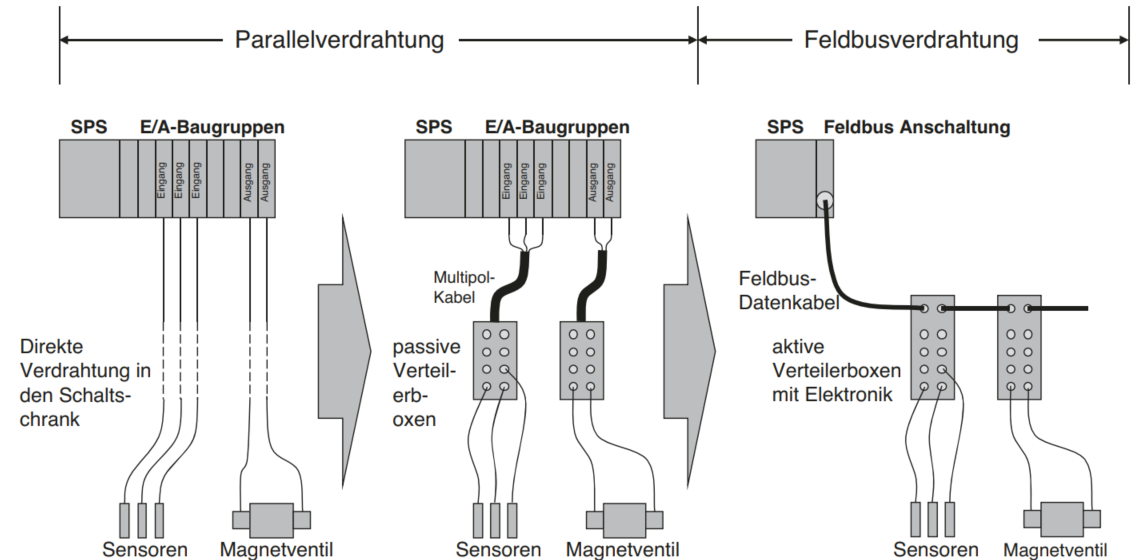
\includegraphics[width=1.0\linewidth]{./images/Parallelverdrahtung_Feldbus.png}
		\caption{Übergang Parallelverdrahtung zu Feldbussen \cite{hering2012elektrotechnik}}
		\label{fig:Parallel_vs_Feldbus}
	\end{figure}\\
	Es haben sich Feldbusse von vielen namhaften Herstellern etabliert. Mittlerweile werden diese Standard-Feldbusse immer weiter von Ethernet basierenden Feldbussen (auch Industrial Ethernet genannt) abgelöst, da diese vor allem Vorteile bezüglich der Übertragungsgeschwindigkeit aufweisen. Die Marktaufteilung aus dem Jahr 2021 ist nachfolgend abgebildet, wobei eine weitere Zunahme der Marktanteile von den Ethernet basierenden Feldbussen zu erwarten ist (vgl. Abbildung \ref{fig:Marktanteil_Feldbus}). \cite{hering2012elektrotechnik} \cite{Marktanteile_HMS}\\
	\begin{figure}[!ht]
		\centering
		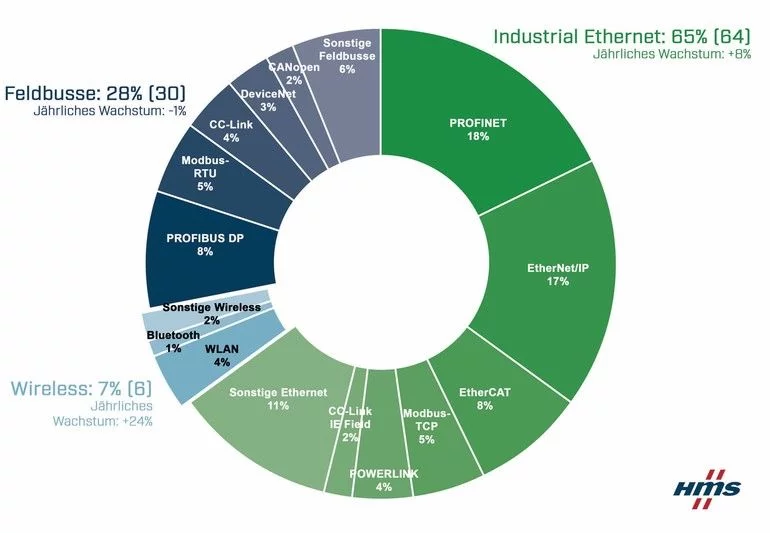
\includegraphics[width=1.0\linewidth]{./images/HMS__Marktanteile_industrielle_Netzwerke.png}
		\caption{Marktanteile Feldbusse und Industrial Ethernet  \cite{Marktanteile_HMS}}
		\label{fig:Marktanteil_Feldbus}
	\end{figure}\\
	\subsection{Standard-Feldbusse}
	\label{subsec:StandardFeldbus}
	In der Anlagentechnik ist die sofortige und zuverlässige Datenübertragung unter anderem aus Gründen der Sicherheit essentiell. Feldbusse sind daher echtzeitfähig. Die Echtzeitfähigkeit besagt, dass die Daten innerhalb einer sehr kurzen festgelegten Zeitspanne, unabhängig von äußeren Einflüssen, übertragen werden müssen. Durch die harte Echtzeit, ist im Gegensatz zur weichen Echtzeit zusätzlich definiert, dass die Daten mit einem absoluten Determinismus übertragen werden müssen. Bei der weichen Echtzeit verlieren die Daten lediglich an Nutzen bei verspätetem Eintreffen, bei der harten Echtzeit werden sie komplett nutzlos. Aus diesem Grund müssen bei der harten Echtzeit 100 \% der Daten innerhalb der definierten Zeit übertragen werden, was insbesondere bei sicherheitsrelevanten Funktionen von Relevanz ist. \cite{dopatka2008framework} \cite{Echtzeit} \\
	Im folgenden sollen ausgewählte gängige Feldbusse kurz erwähnt und erläutert werden.\\
	\textbf{Profibus} wird von dem Dachverband \glqq Profibus \&Profinet International\grqq{} verwaltet, um die Interessen der Nutzer einzubringen. Neben dem Profibus auf Feldbus-Ebene (auch Profibus-DP genannt) existiert eine weitere Variante auf Zellensteuerungs-Ebene und eine auf Prozess-Automatisierungs-Ebene. Als Übertragungstechnik dient der sogenannte RS485-Standard mit einer Zweidrahtleitung. Die Datentransferrate von Profibus beträgt bis zu 12 MBit/s. Speicherprogrammierbare Steuerungen von Siemens setzen häufig Profibus ein.  \cite{hering2012elektrotechnik}\\
	\textbf{CAN-Bus} wurde ursprünglich für die Automobil-Industrie entwickelt und kommt dort heute noch zum Einsatz. Darüber hinaus, nahm die Verbreitung in der Anlagensteuerung zu. Möglich sind Datentransferraten von bis zu 1 MBit/s. Als Übertragungsmedium dient eine Zweidrahtleitung. CAN-Bus zeichnet sich durch eine besonders hohe Datensicherheit, also eine hohe Zuverlässigkeit bei der Datenübertragung aus, weshalb er in der Medizintechnik und Robotik hohen Zuspruch findet. \cite{hering2012elektrotechnik}\\
	\textbf{DeviceNet} basiert auf CAN und ist eine Entwicklung des nordamerikanischen Herstellers \glqq Rockwell Automation\grqq{} . Die Datenübertragungsrate beträgt bis zu 500 kBit/s und die Spannungsversorgung, sowie die Datenkommunikation erfolgen über ein Kabel. \cite{hering2012elektrotechnik}\\
	\textbf{CC-Link} stellt eine Entwicklung von \glqq Mitsubishi\grqq{} dar. Verwaltet wird das Protokoll von einer Anwenderorganisation ähnlich zu Profibus. Die maximale Übertragungsrate beträgt 10 MBit/s und als Übertragungsmedium dient eine dreiadrige Leitung. \cite{hering2012elektrotechnik}\\
	\subsection{Ethernet basierende Feldbusse}
	\label{subsec:EthernetFeldbus}
	Ethernet basierende Feldbusse, häufig auch als \glqq Industrial Ethernet\grqq{} bezeichnet, ermöglichen deutlich höhere Übertragungsraten als Standard-Feldbusse. Daher nimmt deren Verbreitung ständig zu und sie lösen in vielen Bereichen den Standard-Feldbus ab. \cite{hering2012elektrotechnik} \vspace{0.5\baselineskip}\\
	\textbf{Ethernet-Technologie}\\
	Ethernet ist einer von mehreren Standards für die lokale Netzwerkverbindung mittels der \acs{lan}-Technologie (\acl{lan}). Sie ist im IEE 802-3- Standard (Institute of Electrical and Electronis Engineers) genormt. Der Aufbau eines Ethernet-Telegramms ist nachfolgend abgebildet (vgl. Abbildung \ref{fig:EthernetTelegramm}). Die Adressierung erfolgt mittels sogenannter MAC-Adresse oder IP-Adresse (mehr hierzu in Kapitel \ref{sec:TCP/IP}).  \cite{riggert2002rechnernetze}\\ \clearpage
	\begin{figure}[!h]
		\centering
		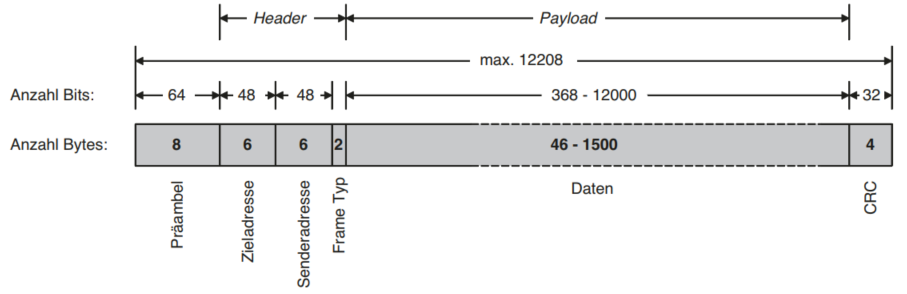
\includegraphics[width=1.0\linewidth]{./images/Ethernet-Telegram.png}
		\caption{Telegramm-Aufbau Ethernet \cite{hering2012elektrotechnik}}
		\label{fig:EthernetTelegramm}
	\end{figure}
	\noindent
	Verschiedene Geräte sind an das Übertragungsmedium angeschlossen und teilen sich dieses. Man spricht von einem Multi-Master-Bus, da jedes Gerät selbständig die Initiative ergreifen kann, um Nachrichten zu senden. Damit jedes Gerät kommunizieren kann und dabei Sendekonflikte vermieden werden, kommt bei Ethernet der \acs{csmacd}-Mechanismus zum Einsatz. \acs{csmacd} steht für \glqq \acl{csmacd}\grqq{} und ermöglicht einen mehrfachen Zugriff (Multiple Access) auf das Übertragungsmedium. \cite{hering2012elektrotechnik} \cite{riggert2002rechnernetze}
	\begin{itemize}
		\item \textbf{Carrier Sense:} Das Übertragungsmedium wird überwacht, damit es nicht durch ein anderes Gerät belegt ist. Erst nachdem das Medium als frei erkannt wird, erfolgt nach einer kurzen Wartezeit die Übertragung. Während des Sendens, wird das Medium weiterhin auf Kollisionen abgehört.
		\item \textbf{Multiple Access:} Es besagt, dass alle Geräte gleichberechtigt auf das Übertragungsmedium zugreifen können.
		\item \textbf{Collision Detection:} Wenn mehrere Geräte zur gleichen Zeit das Übertragungsmedium als frei erkennen kommt es zur Überlagerung, da mehrere Geräte gleichzeitig beginnen zu senden. Dies wird als Kollision bezeichnet und es kommt zur Signalverfälschung durch Überlagerung. Da jeder Sender das Übertragungsmedium während des Sendevorgangs überwacht, wird die Kollision direkt erkannt. Dasjenige Gerät, welches die Kollision erkennt, informiert alle anderen Geräte mittels eines Signales über die aufgetretene Kollision und fordert diese zur Unterbrechung jeglicher Übertragung auf. \\
		Danach warten die Geräte eine zufällige Zeitspanne ab und versuchen das Senden erneut. \cite{riggert2002rechnernetze}
	\end{itemize}
	Durch die Kollision kommt es zu nicht vorhersehbaren Wartezeiten im Sendeprozess. Daher handelt es sich um ein nicht deterministisches Zugriffsverfahren. Ethernet mit \acs{csmacd} ist nicht echtzeitfähig, was wie bereits in Kapitel \ref{subsec:StandardFeldbus} erwähnt, zu Problem bei Automatisierungsanlagen führen kann.\\
	Um die Ethernet-Technologie dennoch in der Automatisierung zu nutzen, haben die Hersteller verschiedene Echtzeitprotokolle entwickelt, um Ethernet echtzeitfähig zu machen. Beispielsweise wird die Methodik \acs{csmacd} außer Kraft gesetzt und stattdessen durch sogenanntes \glqq Pooling\grqq{} oder ein Zeitscheibenverfahren ersetzt. Jeder Hersteller geht hier jedoch seinen eigenen Weg.	Bekannte Ethernet basierende Feldbusse sind \glqq Profinet\grqq{}, \glqq Ethernet/IP\grqq{}, \glqq EtherCAT\grqq{} und \glqq Sercos III\grqq{}.
	EtherCAT ist eine Technologie des Herstellers \glqq Beckhoff\grqq{} , dessen \ac{sps} im Rahmen dieses Projektes zum Einsatz kommt. Aus diesem Grund ist EtherCAT die bevorzugte Technologie und wird im Rahmen dieser Arbeit näher erläutert. \cite{ethercat} \cite{riggert2002rechnernetze}\
	\\
	Weiterhin ist zu beachten, dass die Netzwerktopologie sich bei den Ethernet basierenden Feldbussen häufig von den Standard-Feldbussen unterscheidet. Während bei den Standard-Feldbussen die Anschaltung vorwiegend in der Linienstruktur erfolgt, wird bei der Ethernet Anschaltung oft eine Sternstruktur mit einem Switch eingesetzt (vgl. Abbildung \ref{fig:TopologieEthernet}).
	\begin{figure}[!ht]
		\centering
		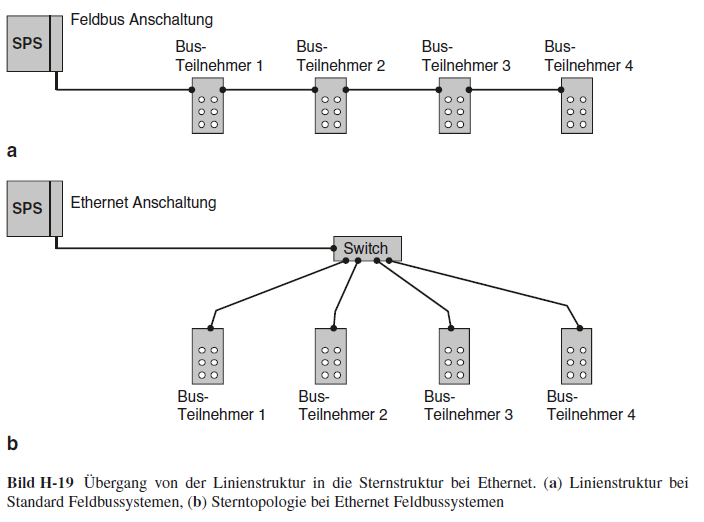
\includegraphics[width=1.0\linewidth]{./images/Feldbus vs Ethernet Anschaltung.png}
		\caption{Topologie: Feldbus (oben), Ethernet basierender Feldbus (unten) \cite{hering2012elektrotechnik}}
		\label{fig:TopologieEthernet}
	\end{figure}\\
	Der Ethernet Switching Hub, abgekürzt als Switch, erlernt beim Einschalten an welchen Ports Teilnehmer angeschlossen sind. Der Switch leitet ein Datentelegramm eindeutig vom Sender zum Empfänger. Dadurch werden von dem Telegramm nicht betroffene Teilnehmer und Ethernet-Segmente nicht unnötig belastet und Kollisionen vermieden. Das Weiterschalten erfolgt auf Basis der Sende- und Ziel-Adresse, welche im Ethernet-Telegramm hinterlegt ist. \cite{hering2012elektrotechnik} \\
	\textbf{EtherCAT} \\
	Wie bereits erwähnt setzen viele Hersteller auf das Zeitscheibenverfahren oder Pooling, um Ethernet echtzeitfähig zu machen. Der Zeitverzug ist hierbei jedoch implementierungsabhängig und kann durch erforderliche technische Komponenten am Bus weiter steigen. Um dies zu verhindern setzt EtherCAT auf einen anderen Lösungsansatz. Im Gegensatz zu anderen Verfahren sollen Daten nicht mehr empfangen, interpretiert und dann wieder weiterversendet werden. Stattdessen setzt EtherCAT auf eine sogenannte \acs{fmmu} (\acl{fmmu}) in jeder E/A-Klemmen. Diese \acs{fmmu} entnimmt nur die relevanten Daten vom Bus, sodass die Telegramme mit einer Verzögerung von nur wenigen Nanosekunden weiterlaufen können. Zum Versenden werden Daten in die durchlaufenden Telegramme eingefügt, sodass es auch hier zu kaum einer Verzögerung kommt. Dieses Prinzip ist nachfolgend dargestellt (vgl. Abbildung \ref{fig:EtherCAT}).
	\begin{figure}[!ht]
		\centering
		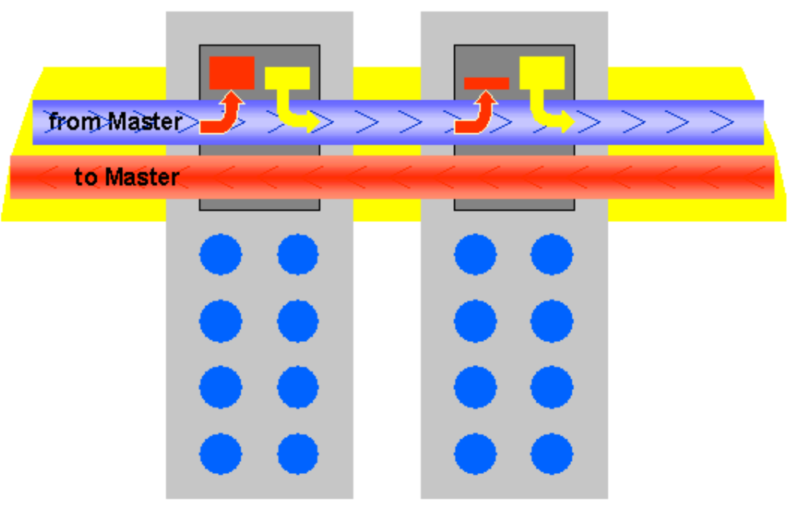
\includegraphics[width=0.7\linewidth]{./images/EtherCAT.png}
		\caption{Telegrammbearbeitung \cite{ethercat}}
		\label{fig:EtherCAT}
	\end{figure}\\
	Dabei wird auf dem gesamten Bus vom Ethernet-Protokoll nach IEE 802.3 nicht abgewichen. Bit-Fehler werden so durch die Prüfsumme erkannt. Neben der Stern-Topologie unterstützt EtherCAT auch eine Linien- oder Baum-Struktur und viele weitere.
	EtherCAT zeichnet sich durch geringe Laufzeitverzögerungen und eine hohe Datenrate aus. Beispielsweise können 1000 E/As in nur 30 \(\mu s\) aktualisiert werden und auch eine Übertragungsrate im GBit-Bereich ist mit Erweiterung möglich. \cite{ethercat}\\
	
	\clearpage
	\section{TCP/IP}
	\ac{tcpip} (\acl{tcpip}) ist das meist verwendete Netzwerkprotokoll weltweit und zudem frei zugänglich. Durch dieses Protokoll wird definiert, wie Daten durch Netzwerkkommunikationshardware versendet und empfangen werden können. Welches Übertragungsmedium verwendet wird ist  nicht definiert, sodass sich neben \ac{lan} z.B. auch WLAN einsetzen lässt.\cite{CS9_TCP} \cite{kim2016service} \\
	\ac{tcpip} ist nicht echtzeitfähig, stellt jedoch eine gute Ergänzung zu den Echtzeitprotokollen dar, um nicht zeitkritische Daten, wie z.B. zur Diagnose oder Visualisierung zu übertragen. Bei \ac{tcpip} handelt es sich um eine sichere Datenübertragung, die Nachrichten in einen Bytestrom verpackt und entpackt. Vom Sender zum Empfänger durchlaufen die Daten vier Schichten (vgl. Abbildung \ref{fig:Schichtenmodell}). Für eine sichere fehlerfreie Übertragung werden die eigentlichen Daten ergänzt um die MAC-/IP- und TCP-Header. Das CRC-Feld stellt eine Art Prüfsumme, mit welcher die Korrektheit der übertragenen Daten überprüft wird. \cite{hering2012elektrotechnik}
	\begin{figure}[!ht]
		\centering
		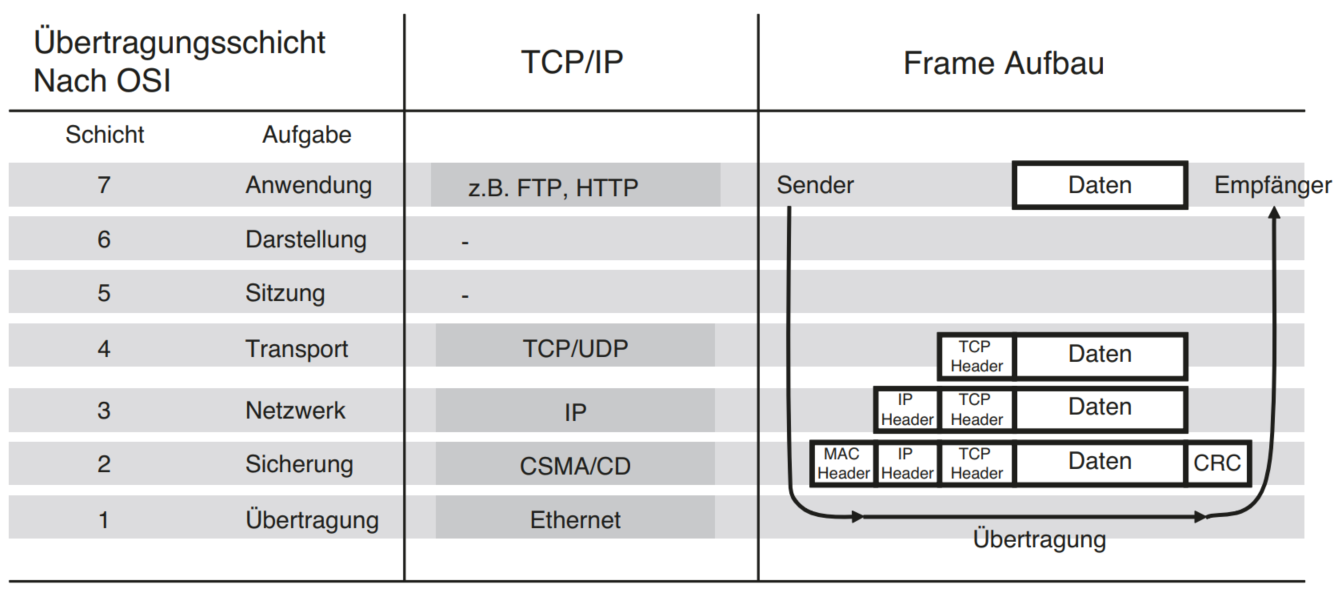
\includegraphics[width=1.0\linewidth]{./images/Schichtenmodell_TCP_IP.png}
		\caption{Schichtenmodell TCP/IP \cite{hering2012elektrotechnik}}
		\label{fig:Schichtenmodell}
	\end{figure} \\
	\ac{tcpip} setzt sich aus den Protokollen \acs{tcp} und \acs{ip} zusammen. \vspace{0.5\baselineskip}\\
	\textbf{TCP}\\
	Das Ziel von \acs{tcp} (\acl{tcp}) ist eine fehlerfreie Datenübertragung. Hierzu muss der Empfänger die korrekt erhaltenen Daten, über eine Nachricht, die an den Sender zugesendet wird, bestätigen. Die Überprüfung der Korrektheit erfolgt mit dem \acs{crc}-Segment. Erhält dieser Sender diese Bestätigung nicht, wird erneut versucht die Daten zu versenden. Hierdurch ist eine fehlerfreie und lückenlose Datenübertragung, selbst bei Netzwerkproblemen garantiert, was jedoch die Prozesse verlangsamt. Eine Alternative zu \acs{tcp} ist \acs{udp} (\acl{udp}). Hierbei erhält der Absender keine Bestätigung, dass die Daten korrekt empfangen wurde. Der Sender fährt direkt mit der Versendung der nächsten Pakete durch. Eine fehlerfreie Übertragung ist nicht garantiert, jedoch ist sie im Vergleich zu \acs{tcp} schneller. Sowohl \acs{tcp}, als auch \acs{udp} bauen auf dem \ac{ip} auf. \cite{CS9_TCP} \vspace{0.5\baselineskip}\\
	\textbf{IP} \\
	Das \ac{ip}-Protokoll arbeitet auf der Internet bzw. \ac{ip}-Schicht des \ac{tcpip}-Protokolls, was der Netzwerkschicht des OSI-Modells entspricht. Die Aufgabe des \acs{ip}-Protokolls ist es, Datenpakete vom Sender zum Empfänger zu übertragen. Eine Datenüberprüfung und Fehlerkorrektur erfolgt nicht, sodass Daten verloren gehen können oder fehlerbehaftet sind. Die Garantie für die korrekte Datenlieferung geschieht durch das \acs{tcp}-Protokoll. Das IP-Protokoll verwendet IP-Adressen, um Netzwerkknoten zu identifizieren. Mit Hilfe derer Adressen wird die Nachricht durch das Netz \glqq geroutet\grqq. Es wird ein idealer Weg zwischen Sender und Empfänger gesucht. \cite{harnisch2009netzwerktechnik} \cite{riggert2002rechnernetze} Es gibt zwei Versionen des IP-Protokolls IPv4 und IPv6. Bei IPv4 besteht die IP-Adresse aus 32 Bit, bei IPv6 aus 128 Bit, was die Anzahl der eindeutigen Adressen erhöht. Aufgrund der zunehmenden Geräteanzahl wird in der Zukunft IPv6 der Standard werden. Heute dominiert jedoch IPv4. \cite{riggert2002rechnernetze} \\
	Eine \acs{mac}-Adresse (\acl{mac}) ermöglicht eine eindeutige Identifikation eines Gerätes im Netzwerk. Da allerdings meist herstellerübergreifende Netzwerke eingesetzt werden, ist die IP-Adresse für eine eindeutige Identifikation besser geeignet. Diese kann entweder manuell oder automatisch zugewiesen werden. Der Aufbau einer IP-Adresse nach IPv4 ist nachfolgend dargestellt (vgl. Abbildung \ref{fig:IP-Adresse}).  \cite{hering2012elektrotechnik} \\
   	\begin{figure}[!ht]
   		\centering
   		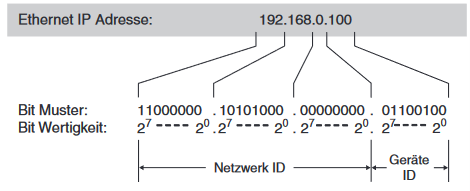
\includegraphics[width=0.70\linewidth]{./images/IP Adresse Aufbau.png}
   		\caption{IP-Adresse Aufbau \cite{hering2012elektrotechnik}} 
   		\label{fig:IP-Adresse}
   	\end{figure}
   	\clearpage
   	\noindent
   	\textbf{Netzwerkarchitektur}\\
   	Während Netzwerke in ihrer Topologie, wie z.B. Bus, oder Stern-Topologie unterschieden werden können, kann auch eine Aufteilung nach Architekturtyp erfolgen. Neben der monolithischen Architektur und der Client-Server-Architektur gibt es Cloud-, Edge- und Fog-Computing. In der monolithischen Architektur existiert nur ein zentraler Rechner. An diesen werden externe Geräte angebunden, die selbst keine Rechenleistung aufweisen. Bei Cloud-, Edge- und Fog-Computing wird ein Teil der Netzwerktechnik an externe Organisationen ausgelagert. Eine externe Organisation kann ein Provider sein, der ein Server bereitstellt. \\
   	Im nachfolgenden soll die Client-Server-Architektur näher erläutert werden, da diese von Relevanz für diese Arbeit ist.
   	Bei der Client-Server-Architektur stellt der Client Anfragen an den Server, welche dieser beantwortet. Dieser Ablauf ist als Sequenzdiagramm in Abbildung \ref{fig:Sequenz Server-Client} dargestellt.\\
   	\begin{figure}[!ht]
   		\centering
   		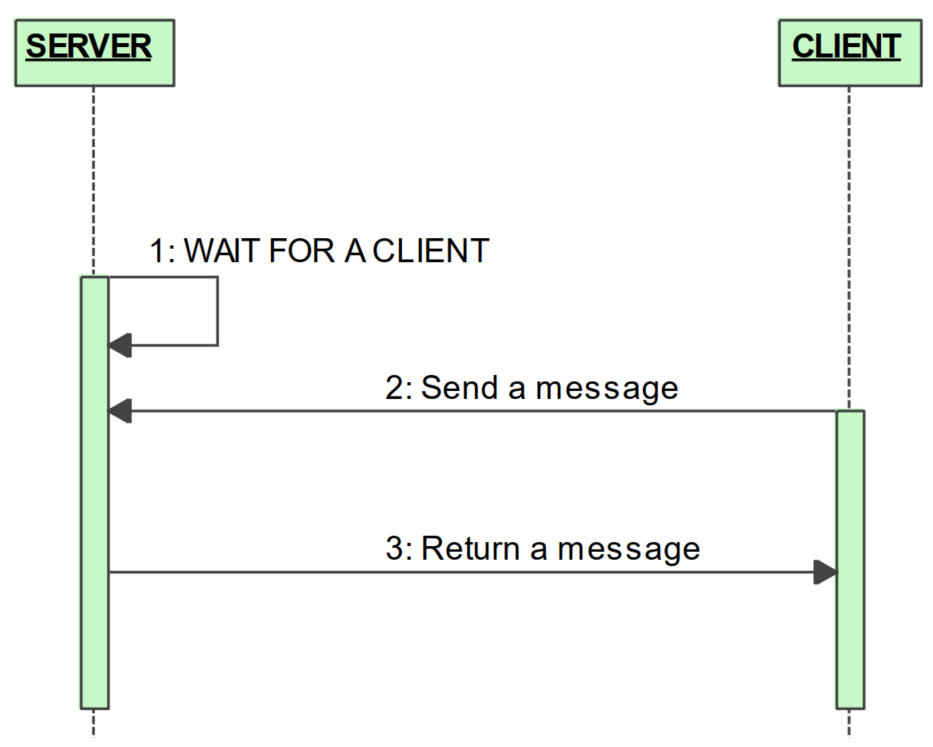
\includegraphics[width=0.50\linewidth]{./images/Sequenzdiagramm_Server_Client.png}
   		\caption{Sequenzdiagramm Server-Client-Architektur \cite{CS9_TCP}} 
   		\label{fig:Sequenz Server-Client}
   	\end{figure} \\   	
   	Charakteristisch für den Server ist dessen vergleichsweise hohe Rechenleistung, was es ermöglicht, dass mehrere Clients zeitgleich auf den Server zugreifen können. Veranschaulichen lässt sich dieses Prinzip mit dem Webbrowser, wie beispielsweise Google Chrome auf dem privaten Rechner. Dieser stellt den Client dar, welcher Anfragen an einen Webserver stellt, um aktuelle Daten passend zu seiner Anfrage zu erhalten. Auf dem Webserver wird beispielsweise ein Online-Shop verwaltet und mehrere Clients können zeitgleich auf diesen zugreifen. Das oben erwähnte Cloud-Computing basiert auf der Client-Server-Architektur, wurde jedoch nutzerfreundlicher gestaltet. \cite{IT-Sicherheit}
   	\label{sec:TCP/IP}
   	\clearpage
   	\section{OPC UA}
   	\acs{opc} (\acl{opc}) ist ein Protokoll zur Maschine-zu-Maschine-Kommunikation, aber auch zur Kommunikation zwischen SPS oder Benutzerschnittstelle und Maschine. Es handelt sich hierbei um einen offenen und plattformunabhängigen Standard, welcher von der \glqq Open Platform Foundation\grqq{} verwaltet wird. OPC UA basiert analog zu TCP/IP auf Ethernet und Internet. Es ist ebenso nicht echtzeitfähig. Das Kommunikationsprotokolls OPC UA ermöglicht eine vertikale und horizontale Kommunikation, da es die einzelnen Automatisierungsebenen verbindet. Somit kann von einem Roboter bis hin zur gesamten Fabriksteuerung alles verbunden werden, was OPC UA beliebt macht, um die Fabrik \glqq Industrie 4.0\grqq{} fähig zu machen. \cite{industrie40} \\
   	OPC UA basiert auf der Server-Client Architektur. Der OPC UA Server kann dann beispielsweise auf der SPS oder der Benutzerschnittstelle laufen und ein Roboter kann als OPC UA Client angebunden werden. Die Daten werden standardisiert und maschinenlesbar semantisch beschrieben, sodass eine herstellerübergreifende Kommunikation problemlos möglich ist. Sensordaten einer Maschine können dadurch an die Anlagensteuerung übertragen und visualisiert werden. OPC UA liefert dabei viele Vorteile: \cite{OPCUA}
   	\begin{itemize}
   		\item \textbf{Sicher:} IT-Sicherheit wurde bei der Entwicklung von OPC UA direkt miteingeplant. Die Kommunikation und der Transport ist sicher und kann über Zugriffsrechte gesteuert werden.
   		\item \textbf{Plattformunabhängig:} Neben der Herstellerunabhängigkeit ist OPC UA unbhängig von der Programmiersprache, was es ermöglicht verschiedene Anlagen einfach zu verknüpfen.
   		\item \textbf{Einfach:} OPC UA ist auf Nutzerfreundlichkeit ausgelegt und das Festlegen von Kommunikationsprotokollen und der Aufbau von Nachrichten entfällt, sodass auch ohne Programmierkenntnisse eine Umsetzung möglich ist. 
   		\item \textbf{Big Data:} OPC UA ermöglicht einfaches Sammeln von Daten aus diversen Maschinen und von unterschiedlichsten Automatisierungsebenen. Hierdurch können sich umfangreiche Potentiale durch die Analyse der Daten ergeben und neue Geschäftsmodelle erschlossen werden. \\
   	\end{itemize}
   	Aufgrund dieser unterschiedlichsten Vorteile, wird OPC UA immer mehr im Bereich Industrie 4.0 eingesetzt. \cite{OPCUA}  \cite{industrie40}
	\clearpage
   	\section{Stäubli-Roboter}
   	Stäubli ist ein in der Schweiz ansässiges Industrieunternehmen, welches in den Bereichen \glqq Elektrische Verbindungen\grqq, \glqq Fluidische Verbindungen\grqq, \glqq Textil\grqq{} und \glqq Robotik\grqq{} tätig ist. Das Produktportfolio im Bereich Robotik umfasst Vier- und Sechsachs-Roboter, sowie kollaborative und mobile Roboter. \cite{StaubliUberUns}\\ Stäubli-Roboter sind nach IP 65 und IP 67 Staub- und Wasser- geschützt, wenn ein Arm mit Überdruckeinheit zum Einsatz kommt. Dies ermöglicht eine gründliche Reinigung aus Hygienezwecken und verhindert das Ansammeln von Staub im Roboter. Beispielsweise ist auch eine Reinigung mit Desinfektionsmittel oder Isopropylalkohol möglich. Zudem können die Roboter mit einem lebensmittelverträglichem Öl eingesetzt werden. Stäubli-Roboter eignen sich daher insbesondere für Anwendungen in der Lebensmittel-, Pharma- und Medizin-Technik, in der viele andere Roboter die Hygieneanforderungen nicht erfüllen. \cite{StaubliProduktubersicht} \vspace{0.5\baselineskip}\\
   	\textbf{Roboter TX2 - 90}\\
   	Im Rahmen dieser Arbeit kommt der Sechsachs-Roboter TX2-90 zum Einsatz (vgl. Abbildung \ref{fig:TX90}). Dieser weist eine Tragkraft von 12 kg und eine Reichweite von 1000 mm auf. Die Wiederholgenauigkeit beträgt 0,03 mm und die maximale kartesische Geschwindigkeit 10,9 m/s. Der Roboter wiegt 114 kg und wird von der Robotersteuerung CS9 mit 2kVA gesteuert. Der Roboter ist für verschiedene, teils auch aggressive Reinigungsmittel geeignet, was für die Lebensmittelindustrie wichtig ist. Die Achsen können maximale Drehmomente zwischen 11 Nm (Achse 6) und 318 Nm (Achse 1) aufbringen. Der Vorderarm des Roboters ist mit vier Magnetventilausgängen, von zwei 5/2-Wege-Magnetventilen versehen. Dies ermöglicht beispielsweise das Öffnen und Schließen eines Greifers.\\
   	Für den Roboter liegt ein Wartungsplan vor, welcher Wartungsarbeiten in unterschiedlichen Intervallen von monatlich bis 5-jährig vorsieht. Diese reichen von einfachen Sichtprüfungen und Bremstests über Ölwechsel und Dichtungstausch bis hin zum Auswechseln von Achsen. \cite{X90}
   	\begin{figure}[h]
   		\centering
   		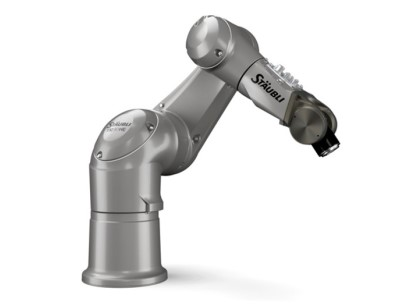
\includegraphics[width=0.50\linewidth]{./images/Staubli_HE.png}
   		\caption{Stäubli TX2 - 90 \cite{Staubli_HE}} 
   		\label{fig:TX90}
   	\end{figure}
   	\subsection{Controller CS9}
   	Der CS9 Controller übernimmt die Steuerung und Versorgung des TX2 - 90 (vgl. Abbildung \ref{fig:CS9}).
   	\begin{figure}[!ht]
   		\centering
   		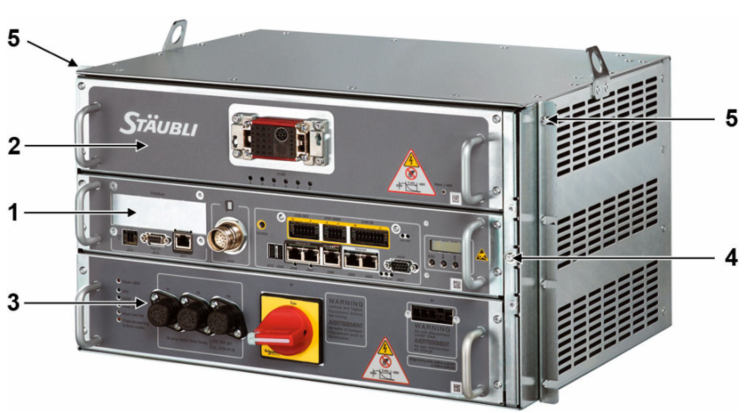
\includegraphics[width=0.70\linewidth]{./images/CS9.png}
   		\caption{Stäubli CS9 Controller \cite{CS9}} 
   		\label{fig:CS9}
   	\end{figure}
   	Der Computer-Einschub (1) beinhaltet Karten, für die Sicherheitssteuerung, Bewegungssteuerung und die externe Kommunikation. Der Verstärker-Einschub (2) wandelt mit Hilfe von digitalen Achsverstärkern Bewegungsvorgaben in Motorströme um. Er beinhaltet zudem die Schnittstelle, an dem der Roboter angeschlossen wird. Der Stromversorgungs-Einschub (3) wandelt die Netzversorgungsspannung für die zuvor genannten Einschübe um und versorgt diese. Zudem existiert ein Anschluss für eine Antistatikmanschette (4), sowie Befestigungsmöglichkeiten (5).
   	\begin{figure}[!ht]
   		\centering
   		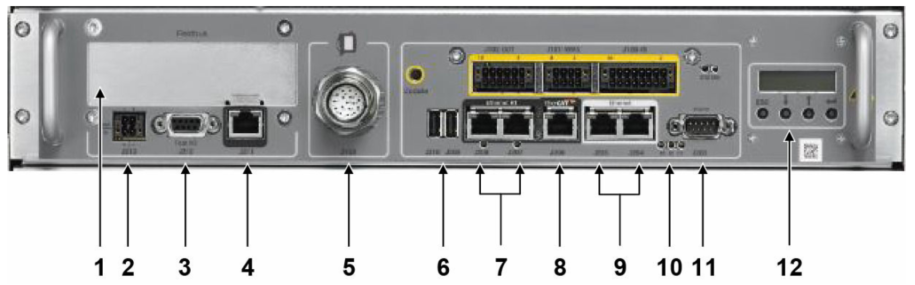
\includegraphics[width=0.70\linewidth]{./images/ComputerEinschub.png}
   		\caption{CS9 Controller Computer-Einschub \cite{CS9}} 
   		\label{fig:ComputerEinschub}
   	\end{figure}
   	Der Computer-Einschub (vgl. Abbildung \ref{fig:ComputerEinschub}) besitzt eine Vielzahl an Kommunikationsschnittstellen, die in der Tabelle nachfolgend dargestellt sind (vgl. Tabelle \ref{table:ComputerEinschub}).
   	\begin{table}[h]
   		\caption{CS9 Controller Computer-Einschub}
   		\label{table:ComputerEinschub}
	   	\begin{tabular}{p{1cm}p{12cm}}
	   		\hline
	   		Nr. & Bezeichnung  \\ [0.5ex] 
	   		\hline
	   		1 & Feldbus, Option für PCIe-Karte  \\ 
	   		2 & Anschluss für optionale externe 24 V Stromversorgung  \\
	   		3 & Schnelle Ein-/Ausgänge  \\
	   		4 & EtherCAT Port (Reserviert) \\
	   		5 & Anschluss Handbediengerät  \\
	   		6 & USB-Ports \\  
	   		7 & Echtzeit-Ethernet-Slave (EtherCAT, Sercos III, EtherNet/IP, PROFINET)  \\ 
	   		8 & EtherCAT-Master  \\ 
	   		9 & Ethernet-Ports (1000 MBits/s und 100 MBits/s)  \\
	   		10 & Status LEDs  \\ 
	   		11 & serielle Verbindung RS232  \\
	   		12 & Benutzerschnittstelle  \\  
	   		\hline
	   	\end{tabular}
	\end{table}
   	An den CS9 Controller kann ein Handbediengerät angeschlossen werden (5), was z.B.  manuelles Verfahren oder einfachere Programmier- und Konfigurationsarbeiten ermöglicht. Hervorzuheben ist zudem der Echtzeit-Ethernet-Slave-Anschluss (7), durch welchen die Steuerung z.B. über EtherCAT mit einer SPS verbunden werden kann. Zusätzlich steht ein EtherCAT-Master-Anschluss (8) zur Verfügung. Die CS9 ermöglicht es somit den Roboter als EtherCAT-Slave oder als EtherCAT-Master zu betreiben. Zudem stehen zwei Ethernet-Ports (9) zur Verfügung, was eine externe Kommunikation z.B. über TCP/IP ermöglicht. Die IP-Adresse der Ethernet-Ports kann frei konfiguriert oder automatisch vergeben werden. Als Dateiübertragungs-Serverprotokoll dient "FTPS+FTP". FTP wird als Standardeinstellung verwendet, während FTPS eine sichere Authentifizierung ermöglicht. \\
   	Auf der CS9-Steuerung lassen sich sogenannte Sockets konfigurieren, welche eine TCP/IP oder eine UDP/IP - Kommunikation ermöglichen. Die Konfiguration kann dabei im Client oder Server-Modus erfolgen. \cite{CS9} Ebenso kann die Steuerung für den Einsatz von OPC UA konfiguriert werden, hierbei kommen jedoch einmalige Lizenzkosten von ca. 500 € pro Roboter hinzu.
   	 
   	\subsection{Programmiersprache VAL 3}
   	Die Programmierung des Roboters kann auf dem Handbediengerät erfolgen oder bevorzugt in der \ac{srs}. In der SRS kann neben der Programmierung eine Simulation des Roboters inklusive 3D-Darstellung erfolgen, sodass die Programme direkt getestet werden können.\\
   	\glqq VAL 3\grqq{} ist eine höhere Programmiersprache und besitzt spezielle Steuerungsfunktionen für den Roboter zur Bewegungsteuerung und zur Ansteuerung von Ein-/Ausgängen. \cite{VAL3} \vspace{0.5\baselineskip}\\
   	\textbf{Programm} \\
   	In einer Applikation können mehrere Programme angelegt werden. Diese verhalten sich wie Funktionen und lassen sich aufrufen. Zur Ausführung der VAL3-Applikation wird standardmäßig das Programm \glqq start()\grqq{} gestartet, welches vergleichbar mit einer \glqq main-Funktion\grqq{} ist. Von hier lassen sich wiederum andere Programme aufrufen. Bei Beendigung der Applikation wird das Programm \glqq stop()\grqq{} einmalig aufgerufen, um z.B. von dort andere Programme zu beenden.\\
   	Programme lassen sich auch als Task ausführen. Bei einer Task handelt es sich um ein Programm welches zu einem gewissen Zeitpunkt ausgeführt wird. Üblicherweise wird die Bewegungssteuerung und die Kommunikation in eigene Tasks ausgelagert. Es wird ein möglichst gleichzeitiges Ausführen der Tasks angestrebt. Da die Steuerung  nur einen Prozess besitzt, ist es jedoch nur möglich eine Task auszuführen. Die augenscheinliche Parallelität, wird dadurch erreicht, dass die Tasks sequentiell sehr schnell hintereinander ausgeführt werden (vgl. Abbildung \ref{fig:tasks}). Dabei wird nicht die gesamte Task abgearbeitet, sondern einige wenige Anweisungen. Eine Task erhält zudem eine Priorität, die angibt, wie viele Programmzeilen ausgeführt werden bis die nächste Task abgearbeitet wird. Eine hohe Priorität sorgt daher für ein schnellstmögliches Abarbeiten dieser Task. Wird in einer Task eine Wartezeit (\glqq delay\grqq) ausgeführt, pausiert diese Task und der Prozessor arbeitet nur die anderen Tasks ab. Neben den erwähnten asynchronen Tasks bietet VAL 3 ebenso synchrone Tasks.\\
   	\begin{figure}[!ht]
   		\centering
   		\includegraphics[width=0.80\linewidth]{./images/tasks.png}
   		\caption{Sequentielle Anordnung von Tasks \cite{VAL3}} 
   		\label{fig:tasks}
   	\end{figure} \vspace{0.5\baselineskip}\\
   	\textbf{Datentypen}\\
   	In VAL 3 gibt es verschiedene einfache Datentypen, die nachfolgend kurz erläutertet werden. Neben den einfachen Datentypen gibt es weitere Datentypen, die z.B. Punkte für die Bewegungsteuerung darstellen. Auf eine Erläuterung dieser wird verzichtet, da diese in der Kommunikation nicht benötigt werden. \clearpage
   	\begin{itemize}
   		\item \textbf{BOOL:} Variablen und Konstanten von diesem Typ können \glqq true\grqq{} und \glqq false\grqq{} annehmen.
   		\item \textbf{NUM:} Datentyp zur Darstellung von numerischen Werten mit 14 signifikanten Stellen. Im Gegensatz zu vielen gängigen Programmiersprachen wird in VAL 3 nicht zwischen verschiedenen Zahlenformaten unterschieden. Dieser Datentyp kann von ganzzahligen Werten bis hin zu Kommazahlen alles abbilden.
   		\item \textbf{BITFELD:} Dieser Datentyp ermöglicht es eine Bitfolge z.B. von booleschen Werten oder digitalen Ein- und Ausgängen kompakt abzuspeichern.
   		\item \textbf{STRING:} In Variablen und Konstanten diesen Typs können Zeichenketten mit einer Länge von bis zu 256 Byte gespeichert werden. Die interne Zeichencodierung erfolgt mit Unicode UTF 8. Bei ASCII-Zeichen entspricht die Länge von 256 Bytes somit 234 Zeichen.
   		\item \textbf{DIO:} Dieser Datentyp ermöglicht es aus dem Programm auf die digitalen Ein-/Ausgänge der Steuerung zuzugreifen. Hierzu speichert die DIO-Variable einen Link zu der entsprechenden Hardware in Form einer physischen Adresse.
   		\item \textbf{AIO:} Mit Hilfe diesen Datentyps können die analogen Ein- und Ausgänge der Steuerung verknüpft werden.
   		\item \textbf{SIO:} Dieser Datentyp ermöglicht es einen seriellen Port oder einen Ethernet Socket Anschluss zu verknüpfen. Dadurch kann beispielsweise eine TCP/IP - Nachricht geschrieben oder gelesen werden, in dem der Variable des Datentyps ein Wert zugewiesen wird oder ein Wert abgelesen wird. \\
   	\end{itemize} \vspace{-15pt}
   	\textbf{Robotersteuerung}\\
   	Neben Funktionalitäten die klassische Programmiersprachen aufweisen, benötigt VAL~3 insbesondere Möglichkeiten, um den Roboterarm zu steuern. Exemplarisch werden einige Befehle kurz vorgestellt.
   	\begin{itemize}
   		\item \textbf{disable / enable Power:} Hiermit lässt sich die Armleistung ab- bzw. einschalten. Für den lokalen, manuellen oder Testbetrieb hat diese Funktion keinen Einfluss.
   		\item \textbf{movej:} Dieser Befehl führt eine Bewegung zu einem Punkt aus. Angegeben werden muss die Winkelposition der Achsen für den Zielpunkt (vom Datentyp \glqq joint\grqq), die Geometrie des Werkzeuges (Datentyp \glqq tool\grqq) und Bewegungsdaten, wie Geschwindigkeit und Beschleunigung (Datentyp \glqq msdec\grqq).
   		\item \textbf{movel:} Dieser Befehl ermöglicht im Gegensatz zum Vorangegangen eine lineare Bewegung. Anstelle der Winkelpositionen als Ziel wird eine kartesische Zielkoordinate (Datentyp \glqq point\grqq) vorgegeben.  \\
   	\end{itemize}
   	\section{Anlagensteuerung}
   	Ein Roboter ist meist nur ein Teil einer Automatisierungslösung. Dieser kann um Förderbänder, Sensoren und andere Aktoren ergänzt werden. Wie die Steuerung dieser Gesamtanlage umgesetzt wird unterscheidet sich von Anlagenautomatisierer zu Anlagenautomatisierer. Hier soll die bei \glqq robomotion\grqq{} gängige Umsetzung aufgezeigt werden, da diese relevant für das Gesamtverständnis und die Konzeptionierung der Komponenten ist. Es erfolgt somit eine Analyse des Ist-Zustandes.\vspace{0.5\baselineskip}\\
   	\textbf{SPS}\\
   	Zentrales Element der Anlagenautomatisierung ist eine Beckhoff-SPS, welche auf einem \ac{ipc} läuft. Diese ist für die Ablauflogik und \glqq Intelligenz\grqq{} der Anlage zuständig. Auf anderen Bestandteilen, wie z.B. der Robotersteuerung ist hingegen nur eine geringe Komplexität abgebildet. In der Robotersteuerung werden meistens Kommandos mit Jobnummern angelegt, wie beispielsweise die Bewegung von Punkt~A zu Punkt~B. Durch den Aufruf der Jobnummer durch die SPS erhält der Roboter den Befehl zur Bewegungsausführung und meldet eine erfolgreich durchgeführte Bewegung der SPS zurück. Welche Bewegungen in welcher Reihenfolge und wann durchgeführt werden, ist dementsprechend nicht in der Robotersteuerung, sondern in der SPS programmiert.\vspace{0.5\baselineskip}\\
   	\textbf{roboTools} \\
   	Weiterer Bestandteil der Automatisierung ist ein Programm namens \glqq roboTools\grqq, welches zur Anlagenvisualisierung dient.\\
   	Dieses läuft auf einem Windows-Betriebssystem in Form einer \ac{wpf}-Anwendung (\acl{wpf}), des \glqq .NET-Frameworks\grqq. Das Programm roboTools mit seiner grafischen Oberfläche enthält verschiedene Diagnosewerkzeuge und kann dem Anlagenbediener Informationen über bspw. Störungen oder der Anlagenauslastung ausgeben und visualisieren. Die Daten hierfür bezieht roboTools überwiegend von der SPS. \vspace{0.5\baselineskip}\\
   	\textbf{roboVision}\\
   	Häufig werden in Anlagen Industriekameras eingesetzt, um die Position von Objekten zu ermitteln oder eine automatisierte Qualitätskontrolle vorzunehmen. Zur Weiterverarbeitung der Kameradaten, um die Position oder die Qualitätsgüte zu bestimmen kommt das Programm \glqq roboVision\grqq{} zum Einsatz. Wie roboTools handelt es sich um ein WPF-Anwendung, welche auf einem Windows-Betriebssystem läuft.\vspace{0.5\baselineskip}\\
   	\textbf{Hardware und Zusammenspiel}\\
   	Sowohl roboTools, als auch roboVision laufen auf einem IPC. Dies kann der selbe IPC sein, auf dem bereits die SPS läuft. Insbesondere für roboVision wird jedoch meist ein eigenständiger leistungsfähiger IPC eingesetzt, da für die Bildverarbeitung eine hohe Rechenleistung zur Verfügung stehen muss. Für die Umsetzung der Kommunikationsschnittstelle, spielt dies jedoch keine große Rolle, da sich alle IPCs in einem Netzwerk befinden. Das Zusammenspiel dieser Komponenten ist nachfolgend dargestellt (vgl. Abbildung \ref{fig:Anlagensteuerung}). Die Kommunikation zwischen Beckhoff-SPS und einer Robotersteuerung erfolgt bei robomotion mit dem Feldbus EtherCAT. Die Kommunikation zwischen der SPS, roboTools und roboVision über ein spezielles Kommunikationsprotokoll namens \acs{ads} (\acl{ads}) von Beckhoff. ADS ermöglicht den Datenaustausch von verschiedenen Systemen über die Netzwerkverbindung, die bereits zwischen der SPS, roboTools und roboVision besteht. \cite{ADS}\\
   	
   	\begin{figure}[h]
   		\centering
   		\begin{tikzpicture}[node distance=2cm]
   			% Erste Reihe von Boxen
   			% Erste Reihe von Boxen
   			\node[draw, rectangle, align=center] (box1) at (2cm,0) {Beckhoff-SPS\\ };
   			\node[draw, rectangle, align=center] (box2) at (7cm,0) {Anlagenvisualisierung\\(roboTools)};
   			\node[draw, rectangle, align=center] (box3) at (-3cm,0) {Bildverarbeitung\\(roboVision)};
   			
   			% Zweite Reihe von Boxen
   			\node[draw, rectangle] (box4) at (2cm,-3cm) {Roboter-Steuerung};
   			\node[draw, rectangle] (box5) at (-3cm,-3cm) {Kamera};
   			
   			% Linien verbinden die Boxen und Beschriftungen hinzufügen
   			\draw (box1) -- node[above] {ADS} (box2);
   			\draw (box1) -- node[above] {ADS} (box3);
   			\draw (box1) -- node[left] {Feldbus} (box4);
   			\draw (box3) -- node[right] {} (box5);
   			
   		
   			
   		\end{tikzpicture}
   		\caption{Anlagensteuerung Aufbau}
   		\label{fig:Anlagensteuerung}
   	\end{figure}
	\clearpage
   	\section{WPF-Anwendung}
   	\label{sec:WPF}
   	Da bereits roboTools und roboVision auf WPF beruhen, ist WPF von großer Relevanz für diese Arbeit.
   	\ac{wpf} (\acl{wpf}) stellt den Nachfolger von Windows Forms dar. Es handelt sich um eine Art Framework und ermöglicht optisch anspruchsvolle Windows-Desktop-Anwendungen zu entwerfen. Die Oberflächenbeschreibung für eine WPF-Anwendung erfolgt mit der Beschreibungssprache \acs{xaml} (\acl{xaml}) (vgl. nachfolgender Codeabschnitt). \cite{kotz2022c}
   	\begin{lstlisting}
   		// XAML-Definition für einen Button
   		<Button Content="Test-Button" Height="74" Width="154"/>
   	\end{lstlisting}
   	WPF basiert auf dem .NET - Framework.\vspace{0.5\baselineskip}\\
   	\textbf{.NET - Framework}\\
   	Das .NET Framework ist eine Plattform für unterschiedliche Programmiersprachen, wie C\# oder Visual Basic  mit denen verschiedene Applikationstypen, wie Desktop, Web oder Mobile entwickelt werden können.\\
   	Das .NET-Framework ist eine Entwicklung von Microsoft. Die meisten Anwendungen können jedoch plattformübergreifend eingesetzt werden. Lediglich Desktopanwendungen, wie z.B. WPF sind an Windows gebunden.  \cite{kotz2022c} \cite{troelsen2022pro}\vspace{0.5\baselineskip}\\
   	\textbf{C\#}\\
   	Das .NET-Framework ist offen für verschiedenste Programmiersprachen, jedoch ist die Verwendung von C\# am geläufigsten und kommt in den vorhandenen Anwendungen von robomotion zum Einsatz. C\# ist eine Entwicklung speziell für .NET und kombiniert Konzepte und Bestandteile von Java, JavaScript, C++ und Visual Basic. Dabei handelt es sich um eine vollwertige objektorientierte Sprache mit Eigenschaften, wie Vererbung und Kapselung. \cite{kotz2022c} \cite{troelsen2022pro}\vspace{0.5\baselineskip}\\
   	\textbf{Programmierumgebung}\\
   	Als Entwicklungsumgebung wird für WPF-Anwendungen vornehmlich Visual Studio eingesetzt. Die integrierte Entwicklungsumgebung Visual Studio wird von Microsoft angeboten und ist daher optimal auf die Entwicklung einer WPF-Anwendung zugeschnitten. Zum Projektzeitpunkt stellt Visual Studio 2022 die aktuellste Version dar. Die \glqq Community Edition\grqq{} ist eine kostenfreie Version für private Projekte, sowie kommerzielle Projekte in Unternehmen mit bis zu 250 Mitarbeitern. \cite{kotz2022c} Als Source-Code-Verwaltungs-Programm wird unternehmensintern \glqq Azure DevOps\grqq{} eingesetzt. Daher wird auch im Rahmen dieser Arbeit auf Visual Studio 2022 in Kombination mit Azure DevOps zurückgegriffen.\\
   	
   	
   	\section{Fazit}
   	Feldbusse ermöglichen eine echtzeitfähige Kommunikation, was für viele Funktionen von großer Bedeutung ist. Die klassischen Feldbusse werden immer mehr von Ethernet basierenden Feldbussen abgelöst. Unternehmensintern kommt neben der SPS der Firma Beckhoff der Ethernet basierende Feldbus EtherCAT zum Einsatz, welcher ebenso eine Entwicklung von Beckhoff darstellt.\\
   	Das TCP/IP- Protokoll stellt eine weitere Möglichkeit zur Datenübertragung dar, ist jedoch nicht echtzeitfähig. Das TCP-Protokoll stellt die korrekte Datenübertragung sicher, weshalb es in der Literatur häufig für Industrieanwendungen, die nicht echtzeitfähig sein müssen zum Einsatz kommt.
   	In einem Paper von Groza und Dragomir \cite{groza2008using} kommt anstelle des TCP-Protokoll das Protokoll UDP zur Übertragung von Live-Kamera-Bildern zum Einsatz, da hier die Schnelligkeit über die Korrektheit zu stellen ist. Teilweise wird in der Literatur VPN zur IT-Sicherheit bei TCP/IP eingesetzt \cite{groza2008using}. OPC/UA stellt eine weitere Möglichkeit zur Datenübertragung dar. Sie überzeugt mit Einfachheit und Flexibilität, bringt aber Mehrkosten mit ohne in diesem konkreten Anwendungsfall mehr als TCP/IP leisten zu können. Zusammengefasst lässt sich sagen, dass TCP/IP für den Anwendungsfall des Übertragens von Fehlermeldungen und Prozessdaten eine gute Lösung darstellt, da hier keine Echtzeitfähigkeit gefordert ist. UDP hingegen soll im Rahmen dieser Arbeit nicht zum Einsatz kommen, da die Korrektheit der Daten über die Schnelligkeit zu stellen ist. Auf den Einsatz von VPN kann verzichtet werden, da die TCP/IP-Kommunikation ausschließlich zwischen Roboter und Anlagenvisualisierung erfolgt und keine Verbindung zum Internet aufweist.\\
   	Weiterer Teil des Projektes ist der Stäubli-Roboter TX2-90 mit dem Controller CS9. Dieser soll in der Programmiersprache VAL~3 in der Entwicklungsumgebung \acl{srs} programmiert werden. Die Gesamtanlage von SPS und Roboter wird ergänzt um ein Visualisierungsprogramm namens roboTools, welches eine Benutzeroberfläche für den Bediener darstellt. roboTools ist eine WPF-Anwendung, die in C\# programmiert ist. Daher soll die zu entwerfende Anwendung, welche die Diagnose und Prozessdaten des Stäubli-Roboters darstellt, ebenso als WPF-Anwendung entwickelt werden. Dies macht eine spätere Integration in roboTools einfach möglich.
   	
	\newpage
	
	\chapter{Anforderungsdefinition}
	\label{chap:Anforderungsdefinition}
	Die Aufgabenstellung und die grobe Anforderungsformulierung soll in diesem Kapitel mit Hilfe eines Lastenheftes in eine strukturierte Form gebracht werden. Das Lastenheft beschreibt, welche Funktionalitäten das zu entwerfende System aufweisen soll. Der Auftragnehmer beschreibt im Pflichtenheft durch welche Systemfunktionalitäten die Aufgaben erfüllt werden sollen und wie die Umsetzung technisch erfolgt. Das Lasten- und Pflichtenheft dient auch zur rechtlichen Absicherung der Vertragsparteien. Obwohl ein Lasten- und Pflichtenheft oft als Vertragsgrundlage entworfen wird und dies im Rahmen des Projektes nicht notwendig ist, soll ein Lastenheft eingesetzt werden. Dies ermöglicht es alle Anforderungen und Rahmenbedingungen zu berücksichtigen und diese im gesamten Projektverlauf im Blick zu behalten. Auf ein Pflichtenheft wird hingegen verzichtet. \cite{SoftwaretechnikBroy}
	Das Lastenheft wird in Muss- und Kann-Kriterien unterteilt. Während bei den Muss-Kriterien eine Erfüllung essentiell ist, stellen die Kann-Kriterien eine optionale Erweiterung dar, die dem System jedoch einen Mehrwert verschaffen.\\
	\begin{longtable}{p{0.5cm}p{10.5cm}p{2cm}}
		\caption{Lastenheft}
		\label{table:Lastenheft}\\
		\hline
		Nr. & Anforderung & Kann/Muss \\ [0.5ex] 
		\hline
		\endhead
		1 & Übertragung von Fehlermeldungen des Stäubli-Roboters an die Anlagenvisualisierung & Muss  \\ 
		2 & Übertragung von Prozessdaten des Stäubli-Roboters an die Anlagenvisualisierung & Muss  \\
		3 & Übertragung von Daten z.B. Kameradaten von der Anlage an den Stäubli-Roboter & Muss  \\
		4 & Ausgabe der Roboterfehler auf der Anlagenvisualisierung in verständlicher Form (ausformuliert, Fehlercode genügt nicht) & Muss  \\
		5 & Funktionierende Feldbusverbindung zwischen Stäubli-Roboter und SPS & Muss  \\
		6 & Funktionierende TCP/IP Kommunikation zwischen Stäubli-Roboter und Anlagenvisualisierung & Muss  \\  
		7 & Abspeichern der Fehler und der Daten in log-File & Muss  \\ 
		8 & Fehlerfreie und prozesssichere Kommunikation & Muss  \\ 
		9 & Einsatz von mehreren Stäubli-Robotern zeitgleich  & Kann  \\
		10 & Vorgabe von der Anlagenvisualisierung, wie häufig Daten versendet werden sollen & Kann  \\
		11 & Vorgabe von der Anlagenvisualisierung, ab welcher Schwere Systemereignisse versendet werden sollen & Kann  \\ 
		12 & Visualisierung der Daten & Kann  \\
		13 & Verwertung der Daten z.B. für Warnungen & Kann  \\  
		14 & Übersichtliche Darstellung aller Daten und Meldungen & Kann  \\ 
		15 & Melden, dass Bahnpunkte umgeteacht wurden & Kann  \\ 
		\hline
	\end{longtable}
	\noindent Im Rahmen dieser Arbeit ist die Feldbus-Verbindung zwischen SPS und Roboter zu entwerfen. Der Fokus liegt jedoch auf der TCP/IP-Verbindung zwischen Roboter und Anlagenvisualisierung. Darüber hinaus ist das Programm für den Roboter zu konzeptionieren und zu implementieren.\\
	Das andere Ende der TCP/IP-Verbindung stellt die Anlagenvisualisierung dar. Dort sollen die Fehlermeldungen ausgegeben und die Daten visualisiert werden. Als Anlagenvisualisierung dient bei robomotion roboTools. Die zu entwerfende WPF-Anwendung zur TCP/IP-Kommunikation und zur Datenvisualisierung kann nach Projektende in roboTools integriert werden. Dies soll jedoch nicht mehr Teil der Arbeit sein. Die zu entwerfende WPF-Anwendung wird im Rahmen dieser Arbeit vereinfacht als Anlagenvisualisierung bezeichnet.\\
	Die bestehende Anwendung roboVision erstellt auf Basis von Kamerabildern Positionsdaten von zugreifenden Objekten. Diese Positionsdaten können über die Beckhoff-spezifische Verbindung \acs{ads} zur Anlagensteuerung übertragen werden und somit auch von der zu entwerfenden WPF-Anwendung abgegriffen werden. Alternativ kann später auch ein direktes Versenden der Positionsdaten von der Anlagenvisualiserung zum Roboter umgesetzt werden. Dafür kann auf den entwickelten Source-Code der Anlagenvisualisierung zurückgegriffen werden. Einfachheitshalber wird in dieser Arbeit angenommen, dass die Positionsdaten in der Anlagenvisualisierung vorhanden sind und von dort direkt versendet werden können.\\
	Eine Konzeptionierung und Implementierung des SPS-Programms kann entfallen, da die Kommunikation mit einer Feldbus-Verbindung in der Beckhoff-SPS bei robomotion Stand der Technik ist und dadurch aus anderen Projekten übernommen werden kann. Das Zusammenspiel all dieser Komponenten ist nachfolgend dargestellt, wobei die im Rahmen dieser Arbeit zu entwerfenden Komponenten farbig markiert sind (vgl. Abbildung \ref{fig:Anlagensteuerung_Aufgabe}).
	\begin{figure}
		\centering
		\begin{tikzpicture}[node distance=2cm]
			% Erste Reihe von Boxen
			% Erste Reihe von Boxen
			\node[draw, rectangle, align=center] (box1) at (3cm,0) {Beckhoff-SPS\\ };
			\node[draw, rectangle, align=center, fill=green!20] (box2) at (9cm,0) {Anlagenvisualisierung\\(spätere Integration in roboTools)};
			\node[draw, rectangle, align=center] (box3) at (-3cm,0) {Bildverarbeitung\\(roboVision)};
			
			% Zweite Reihe von Boxen
			\node[draw, rectangle, fill=green!20] (box4) at (3cm,-3cm) {Roboter-Steuerung};
			\node[draw, rectangle] (box5) at (-3cm,-3cm) {Kamera};
			
			% Linien verbinden die Boxen und Beschriftungen hinzufügen
			\draw (box1) -- node[above] {ADS} (box2);
			\draw (box1) -- node[above] {ADS} (box3);
			\draw (box1) -- node[left, fill=green!20] {Feldbus} (box4);
			\draw (box2) -- node[right, fill=green!20] {TCP/IP} (box4);
			\draw (box3) -- node[right] {} (box5);
		\end{tikzpicture}
		\caption{Gesamtanlage zu entwerfende Komponenten}
		\label{fig:Anlagensteuerung_Aufgabe}
	\end{figure}

	
	\chapter{Konzeptionierung}
	In diesem Kapitel sollen die Kommunikationsverbindungen, sowie das Roboterprogramm und die Anlagenvisualisierung konzeptioniert werden. Hierfür werden die Komponenten der Anlage benannt und ihre Funktionen grob skizziert. Dies erfolgt mit Hilfe eines UML-Klassendiagramms (vgl. Abbildung \ref{fig:UMLKlassenAnlage}). \acs{uml} (\acl{uml}) ermöglicht eine Systemmodellierung mit Hilfe von grafischer Notation \cite{Sommerville}.
	\begin{figure}
		 \begin{tikzpicture}
		 	\umlclass[x=0]{SPS}{
		 		- Eingänge : int \\
		 		- Ausgänge : bool \\
		 	}{
		 		+ sendeBefehle() : void \\
		 		+ empfangeBestätigungen() : void
		 	}
		 	
		 	\umlclass[x=8]{Anlagenvisualisierung}{
		 		- Betriebsmodus : string \\
		 		- Logger : string\\
		 		- Graphik: \\
		 		
		 	}{
		 		+ erfrageRoboterDaten() : void \\
		 		+ empfangeRoboterDaten() : void \\
		 		+ sendePositionen(): void\\
		 		+ visualisiereFehlermeldungen(): void\\
		 		+ visualisiereRoboterdaten(): void \\
		 		+ schreibeLogFile(): void
		 	}
		 	\umlclass[x=4, y=-7]{Roboter}{
		 		- Geschwindigkeit : float \\
		 		- Temperatur: int \\
		 		- Drehmoment: int \\
		 		- Fehlermeldung: string
		 	}{
		 		+ bewegen() : void \\
		 		+ empfangeBefehle() : void \\
		 		+ sendeBestätigungBewegungsausführung(): void\\
		 		+ sendeDaten(): void \\
		 		+ sendeFehlermeldungen(): void
		 	}
		 	% Verbindungslienie zwischen SPS und Roboter mit Multiplicitäten
		 	\umluniassoc[pos=0.5]{Roboter}{SPS}
		 	\umluniassoc[pos=0.5]{SPS}{Roboter}
		 	
		 	\umluniassoc[pos=0.5, anchor1=145,anchor2=90]{Anlagenvisualisierung}{SPS}
		 	\umluniassoc[pos=0.5, anchor1=90,anchor2=145]{SPS}{Anlagenvisualisierung}
		 	
		 	\umluniassoc[pos=0.5]{Anlagenvisualisierung}{Roboter}
		 	\umluniassoc[pos=0.5]{Roboter}{Anlagenvisualisierung}
		 	
	
		 \end{tikzpicture}
		 \caption{UML-Klassendiagramm Gesamte Anlage}
		 \label{fig:UMLKlassenAnlage}
	\end{figure}
	Das UML-Diagramm zeigt die Komponenten SPS, Roboter und Anlagenvisualisierung auf. Die Kommunikation zwischen SPS und Roboter erfolgt mittels Feldbus, zwischen Anlagenvisualisierung und Roboter mittels TCP/IP. Daher soll im ersten Schritt der Feldbus und die TCP/IP-Verbindung konzeptioniert werden. Erst anschließend kann das Programm des Roboters und der Anlagenvisualisierung konzeptioniert werden, da dieses maßgeblich abhängig von der Wahl und dem Aufbau der Kommunikationsverbindung ist. Nachdem die Feldbus-Verbindung und die TCP/IP-Verbindung konzeptioniert wurden sollen die zu übertragenden Daten für die TCP/IP-Verbindung konzeptioniert werden. Anschließend erfolgt die Konzeptionierung der Software für den Stäubli-Roboter und die Anlagenvisualisierung.
	 
	\section{Feldbus-Verbindung}
	\label{sec:KonzeptFeldbus}
	Aufgabe der Feldbusverbindung ist es, die Kommunikation zwischen dem Stäubli-Roboter und der Beckhoff-SPS sicherzustellen. Hierzu werden einerseits Befehle, wie zur Bewegungsdurchführung zum Roboter übertragen, andererseits Informationen, wie z.B. eine Bestätigung der vollendeten Bewegung zurück an die SPS gesandt.\\
	\textbf{Wahl des Feldbusses}\\
	In Kapitel \ref{sec:Feldbus} wurden die Feldbusse in Standard-Feldbusse und Ethernet basierende Feldbusse unterteilt. Die Wahl fällt hierbei auf einen Ethernet-basierenden Feldbus, weil dies der aktuelle Stand der Technik darstellt und zudem firmenintern ausnahmslos eingesetzt wird. Nach Kapitel \ref{subsec:EthernetFeldbus} sind Profinet, Ethernet/IP, EtherCAT und Sercos III häufig eingesetzte Ethernet basierende Feldbusse. Eine Gegenüberstellung der Vor- und Nachteile der einzelnen Feldbusse und eine Auswahl anhand dieser Kriterien kann jedoch entfallen, da zwei Argumente für den Einsatz von EtherCAT, alle anderen Kriterien überwiegen.\\
	Im Projekt kommt eine Beckhoff-SPS zum Einsatz. EtherCAT ist eine Entwicklung von Beckhoff und daher bestmöglichst auf die SPS von Beckhoff abgestimmt.\\
	Darüber hinaus, kommt unternehmensintern EtherCAT bereits in anderen Projekten zum Einsatz. Die Wahl von EtherCAT bringt daher folgende Vorteile mit sich:
	\begin{itemize}
		\item \textbf{Know How: } Firmenintern hat sich durch den wiederholten Einsatz von EtherCAT bereits eine große Wissenbasis und Erfahrung aufgebaut. Bei schwerwiegenderen Problemen ermöglicht dies eine einfachere Fehlersuche.
		\item \textbf{Schulungszwecke: } Durch andere Projekte sind beispielsweise die Service-Techniker bereits in EtherCAT geschult. Die Buchung einer zeit- und kostenintensiven Schulung für einen anderen Feldbus kann entfallen.
		\item \textbf{Standardisierung:} Der Einsatz von vielen unterschiedlichen Systemen innerhalb des Unternehmens erhöht den Aufwand in Dokumentation und Einkauf. Daher wird versucht die Varianz möglichst gering zu halten und auf einen unternehmensinternen Standard, welcher bereits häufig verwendet wird zu setzen.\\
	\end{itemize}
	\textbf{Master-Master vs. Master-Slave}\\
	Standardmäßig wird im Auslieferungszustand sowohl die Beckhoff-SPS, als auch der Stäubli Roboter als Master eingesetzt.	Jedoch ist EtherCAT rein für Master-Slave- Kommunikation ausgelegt, d.h. es kann nur ein Master existieren. \cite{ethercat}	Beckhoff bietet jedoch eine spezielle Bridge-Klemme (EL6692) an, die es erlaubt EtherCAT-Stränge zu synchronisieren und ein Datenaustausch zwischen den einzenen Strängen zu ermöglichen. Da jeder EtherCAT-Strang einen eigenen Master besitzt ermöglicht die Bridge den Einsatz von mehreren Mastern. \cite{Bridge} Hierdurch entstehen jedoch zusätzliche Kosten und auch die Komplexität des Systems steigt. Da sowohl die Stäubli-Steuerung, als auch die SPS ebenso als Slave konfiguriert werden kann, fällt die Entscheidung auf die Master-Slave-Kommunikation, um die zusätzliche Master-Master-Klemme einzusparen.\\
	\textbf{Wahl des Masters} \\
	Nachdem die Entscheidung für eine Master-Slave-Architektur gefallen ist, muss festgelegt werden, ob die Beckhoff-SPS oder der Stäubli-Roboter als Master konfiguriert wird. Da der Einsatz von mehreren Stäubli-Robotern in Automatisierungslösungen denkbar ist, könnte nicht jeder Stäubli-Roboter als Master eingesetzt werden. Folglich wäre ein Stäubli-Roboter der Master, die anderen Stäubli-Roboter, sowie die SPS Slaves. Um diese Unterschiede in den einzelnen Stäubli-Robotern zu verhindern, ist es sinnvoll die Beckhoff-SPS als Master zu konfigurieren, sodass alle Stäubli-Roboter einheitlich als Slaves eingesetzt werden. Darüber hinaus ist die SPS der zentrale Teil der Anlagenautomatisierung. Von ihr können weitere Komponenten, wie Roboter anderer Hersteller gesteuert werden, weshalb die Wahl der SPS als Master sinnvoll ist.\\
	Die Gesamtentscheidung zur Konfiguration ist nachfolgend mit Hilfe eines morphologischen Kastens dargestellt.\\
	\begin{table}
		\caption{Morphologischer Kasten Feldbus}
		\label{table:MorphoFeldbus}
		\centering
		\begin{tabular}{
				>{\columncolor{gray!20}}p{2.5cm}
				>{\centering\arraybackslash}p{2.5cm}
				>{\centering\arraybackslash}p{2.5cm}
				>{\centering\arraybackslash}p{2.5cm}
				>{\centering\arraybackslash}p{2.5cm}
			}
			\toprule
			\textbf{Merkmal} & \textbf{Option 1} & \textbf{Option 2} &  \textbf{Option 3}&  \textbf{Option 4}\\
			\midrule
			Bussystem & \cellcolor{green!10}EtherCAT & Profinet & Sercos III & Ethernet/IP\\
			\hline
			Architektur & Master-Master & \cellcolor{green!10}Master-Slave & &\\ \hline
			Master & \cellcolor{green!10}SOS & Stäubli & &\\
			\bottomrule
		\end{tabular}
	\end{table}
	
	
	
	\section{TCP/IP-Verbindung}
	\label{sec:KonzeptTCPIP}
	Nachdem die Feldbus-Verbindung konzeptioniert wurde, erfolgt die Auslegung der TCP/IP-Verbindung. Hierbei müssen viele Einzelentscheidungen getroffen werden, welche am Ende mit einem morphologischen Kasten zusammengefasst dargestellt werden.\\
	\textbf{Wahl der Architektur} \\
	Wie in Kapitel \ref{sec:TCP/IP} erläutert kommt für eine TCP/IP-Verbindung die Client-Server-Architektur zum Einsatz. Dabei kann entweder der Stäubli-Roboter oder die Anlagenvisualisierung als Server dienen. In der Literatur wird meist empfohlen, die Seite mit der höheren Rechenleistung als Server einzusetzen (vgl. Kapitel \ref{sec:TCP/IP}). Dies stellt in diesem Fall die Anlagenvisualisierung dar. Wenn hingegen der Roboter als Server dienen würde und es zum Einsatz von mehreren Roboter kommen würde, wäre der Einsatz von mehreren Client-Instanzen auf der Anlagenvisualisierung notwendig oder die anderen Roboter müssten als Client konfiguriert werden. Daher eignet sich die Anlagenvisualisierung besser als Server und die einzelnen Roboter werden als Client konfiguriert. \\
	\textbf{Nachrichtentypen}\\
	Für folgende Daten, die übertragen werden müssen, muss festgelegt werden, ob und wie diese auf einzelne Nachrichten aufgeteilt werden.
	\begin{itemize}
		\item \textbf{Systemereignisse: } Erfasste Meldungen, wie z.B. Fehler müssen von dem Roboter zu der Anlagenvisualisierung übertragen werden.
		\item \textbf{Prozessdaten: } Vom Roboter erfasste Daten, wie Temperaturen oder digitale Werte, wie Fehler an den Ventilen müssen vom Roboter zur Anlagenvisualisierung übertragen werden.
		\item \textbf{Kameradaten:} Positionsdaten von zugreifenden Objekten, welche durch Kameradaten generiert werden, müssen von der Anlagenvisualisierung zum Roboter übertragen werden.\\
		\item \textbf{Aktualisierung Systemereignis-Schwere:} Die Anlagenvisualisierung soll vorgeben können ab welcher Schwere die Roboter Systemereignisse versenden sollen. Hierdurch können z.B. vergleichsweise unkritische Informationsmeldungen von dem Versand ausgeschlossen werden. Hierfür muss übertragen werden, ab welcher Schwere, der Roboter das Systemereignis senden soll.\\
	\end{itemize}
	Da die Kameradaten in die entgegengesetzte Richtung, wie die anderen Daten übertragen werden, werden diese in eine eigene Nachricht verpackt. Die Systemereignisse und die Prozessdaten können in einer Nachricht oder in getrennten Nachrichten versandt werden. Da die Prozessdaten durchgängig anfallen, die Systemereignisse jedoch azyklisch lohnt sich eine Trennung.\\
	Die Prozessdaten wiederum können gebündelt oder getrennt in einzelne Nachrichten z.B. für die Temperaturen und die digitalen Werte, versendet werden. Da beispielsweise Temperaturen nicht besonders dynamisch sind könnte die Übertragungsfrequenz für diese Daten geringer sein, was die Auslastung der Verbindung reduzieren würde. Dies erhöht jedoch die Komplexität, da viele verschiedene Nachrichtentypen anfallen, was bei Wartungen oder Änderungen in späteren Jahren zum Problem werden kann. Da das zyklische Versenden aller Prozessdaten, die Übertragungsrate der TCP/IP-Verbindung nicht übersteigen wird, fällt die Entscheidung auf das Zusammenfassen aller Prozessdaten in einer Nachricht. Folglich gibt es drei Nachrichtentypen: Kameradaten, Systemereignisse und Prozessdaten.\\
	\textbf{Auslöser für Versand der Systemereignisse}\\
	Die Systemereignisse können entweder zyklisch z.B. einmal pro Sekunde zusammengefasst, oder direkt bei Auftreten versendet werden. Die Entscheidung fällt auf ein direktes Versenden bei Auftreten, damit wichtige Fehlermeldungen schnellstmöglich ankommen. Zudem handelt es sich um ein azyklisches Ereignis, d.h. die Systemereignisse werden nur sporadisch versendet.\\
	\textbf{Auslöser für Versand der Prozessdaten}\\
	Die Prozessdaten werden zyklisch benötigt und sind nicht abhängig von besonderen Ereignissen. Ein zyklischer Versand bietet sich hier an. Die Sendefrequenz muss dann in jedem Stäubli-Roboter einprogrammiert werden und ist dann fest eingestellt. Vorteilhaft wäre es wenn die Sendefrequenz von dem Server Anlagenvisualisierung vorgegeben werden kann. Dadurch kann die Sendefrequenz angepasst und z.B. zur Fehlerfindung erhöht werden. Darüber hinaus kann die Änderung an dieser zentralen Instanz erfolgen und muss nicht manuell bei jedem einzelnen Stäubli-Roboter durchgeführt werden. Dies ist insbesondere praktisch, wenn ein Zugriff über das Fernwartungssystem auf die Anlagenvisualisierung erfolgt. Daher soll ein Datenanforderungstelegramm zyklisch von der Anlagenvisualisierung an alle Clients (Stäubli-Roboter) gesandt werden. Diese sollen nach Erhalt der Anforderung ein Prozessdatentelegramm versenden. Der Einsatz von Datenanforderungstelegrammen bringt ein weiteren Vorteil mit sich. Durch die Zeitdifferenz zwischen Datenanforderungstelegramm und Erhalt des Datentelegramms kann überprüft werden, ob die Datenübertragung ausreichend stabil ist und ob der Client noch verbunden ist. Wenn innerhalb einer vorgegeben Zeitspanne keine Antwort in Form des Datentelegramms erfolgt kann eine Warnung ausgegeben werden, dass dieser Stäubli-Roboter nicht erreichbar ist.\\
	\textbf{Auslöser für Versand von Kameradaten} \\
	Beim Anfallen von Positionsdaten, welche anhand von Kameradaten berechnet werden, sollen diese schnellst möglichst an den Roboter übertragen werden. Aus diesem Grund erfolgt der Versand dieser Daten ereignisgesteuert, d.h. direkt nach Erhalt der Positionsdaten wird ein Telegramm an den entsprechenden Roboter gesandt.\\
	\textbf{Auslöser für Versand Aktualisierung Systemereignis-Schwere} \\
	Sobald erstmalig eine TCP/IP-Verbindung mit einem Roboter aufgebaut wurde, soll ein Telegramm für die Aktualisierung der Schwere versendet werden. Ebenso nach einem Verbindungsabbruch mit anschließendem Verbindungsaufbau. Der Roboter speichert die Schwere ab.
	\newline
	Die Entscheidungsfindung bei den eben genannten Auswahlmöglichkeiten ist in einem morphologischen Kasten (vgl. Tabelle \ref{table:MorphoTCPIP}) dargestellt.
	
	\begin{table}
		\caption{Morphologischer Kasten TCP/IP-Verbindung}
		\label{table:MorphoTCPIP}
		\centering
		\begin{tabular}{
				>{\columncolor{gray!20}}p{3cm}
				>{\centering\arraybackslash}p{3.5cm}
				>{\centering\arraybackslash}p{3.5cm}
				>{\centering\arraybackslash}p{3.5cm}
			}
			\toprule
			\textbf{Merkmal} & \textbf{Option 1} & \textbf{Option 2} &  \textbf{Option 3}\\
			\midrule
			Architekturwahl & \cellcolor{green!10}Anlage = Server & Roboter = Server &\\
			\hline
			Nachrichtentypen & Eine Nachricht für Alles & Prozessdaten unterteilt & \cellcolor{green!10}Prozessdaten und Systemereignisse getrennt\\ \hline
			Auslöser Versand Systemereignisse & Zyklisch & \cellcolor{green!10}Ereignisbasiert & \\ \hline
			Auslöser Versand \newline Prozessdaten & \cellcolor{green!10}Anforderungs-telegramm & Zyklisch &  \\ \hline
			Auslöser Versand\newline Kameradaten & Zyklisch & \cellcolor{green!10}Ereignisbasiert&  \\
			\bottomrule
		\end{tabular}
	\end{table}
	\noindent
	\textbf{Nachrichtenaufbau Datentelegramm}\\
	Nachfolgend soll der Nachrichtenaufbau des Datentelegramms festgelegt werden. Durch Brainstorming und durch Inspiration von anderen Telegram-Aufbauten wie Ethernet (vgl. Kapitel \ref{subsec:EthernetFeldbus}) werden verschiedene Möglichkeiten des Telegrammaufbaus entworfen:
	\begin{itemize}
		\item \textbf{Konzept 1:} <Nachrichten-ID>,<Sender-ID>,<Uhrzeit>,<Daten>
		\item \textbf{Konzept 2:} <Nachrichten-ID>,<Sender-Name>,<Daten>
		\item \textbf{Konzept 3:} <Eindeutige ID (GUID)>,<Sender-ID>
		<Daten>
		\item \textbf{Konzept 4:} <Nachrichten-ID>,<Sender-ID>,<Daten>,<CRC>
		\item \textbf{Konzept 5:} <Nachrichten-ID>,<Sender-ID>,<Daten Gleitkomma, dynamisch>
	\end{itemize}
	In Konzept 1, 2, 4 und 5 existiert eine Nachrichten-ID am Anfang, damit der Empfänger weiß, dass es sich z.B. um ein Datentelegramm und kein Systemereignis handelt. Anschließend folgt die Sender-ID, damit der Server weiß von welchem Roboter die Daten stammen.\\
	Bei Konzept 2 wird die Sender-ID, welche durch eine Zahl dargestellt wird, durch einen konfigurierbaren Namen ersetzt, was die Nutzerfreundlichkeit erhöht, da bei späterer Wartung ggf. unbekannt ist, welcher Roboter welche Nummer besitzt. \\
	Bei Konzept 1 wird darüber hinaus die Uhrzeit mit versendet, dies ist für Dokumentationszwecke sinnvoll und ebenso kann eine Zeitdifferenz zwischen Roboter und Anlagenvisualisierung detektiert werden. Das Datum kann durch die Anlagenvisualisierung bei Erhalt der Nachricht bestimmt werden und muss daher nicht versendet werden. \\
	Bei Konzept 4 wird zusätzlich ein CRC-Segment versendet. Im CRC-Segment wird eine Prüfsumme übermittelt, welche vom Sender aus der zu übermitteltenden Nachricht berechnet wird. Der Empfänger berechnet die Prüfsumme aus der erhaltenen Nachricht und vergleicht sie mit dem CRC-Segment, um zu überprüfen, ob die Nachricht korrekt übermittelt wurde. TCP/IP stellt jedoch bereits selbständig eine fehlerfreie Übertragung durch ein CRC-Segment sicher. Durch eine zusätzliche Prüfsumme kann zwar die Sicherheit bezüglich des korrekten Einlesens der Daten erhöht werden, für die Übertragung selbst ist ein CRC-Segment jedoch nicht mehr notwendig. \\
	Konzept 3 sieht den Einsatz einer eindeutigen ID vor. Mit jedem Datenanforderungstelegramm wird eine eindeutige ID generiert. Der Roboter antwortet mit der Rücksendung des selben ID und den angehängten Daten. Dadurch kann eine bessere Zuordnung der Datentelegramme zu den Aufforderungen erfolgen, um sicherzustellen, dass die Datentelegramme nicht hinterherhinken.\\
	Die fünf entworfenen Konzepte zum Nachrichtenaufbau werden nachfolgend verglichen (vgl. Tabelle \ref{tab:nachrichtenaufbau-vergleich}). Zum Einsatz kommen Harvey-Balls, die den Erfüllungsgrad des jeweiligen Kriteriums wiedergeben. Alle Kriterien haben eine ähnliche Wichtigkeit, mit der sich abschließend eine Gesamtwertung ermitteln lässt. 4 entspricht dabei der höchsten Wertung mit einem durchschnittlich komplett ausgefüllten Harvey-Ball.
	\begin{table}[h]
		\centering
		\caption{Vergleich Nachrichtenaufbau}
		\label{tab:nachrichtenaufbau-vergleich}
		\begin{tabularx}{\linewidth}{p{0.2\linewidth} >{\centering\arraybackslash}X >{\centering\arraybackslash}X >{\centering\arraybackslash}X >{\centering\arraybackslash}X >{\centering\arraybackslash}X}
			\hline
			\textbf{ } & \textbf{1} & \textbf{2} & \textbf{3} & \textbf{4} & \textbf{5}\\
			\hline
			Informationsgehalt & \harveyBallThreeQuarter & \harveyBallHalf & \harveyBallHalf & \harveyBallHalf & \harveyBallThreeQuarter\\
			Übertragungssicherheit & \harveyBallThreeQuarter & \harveyBallThreeQuarter & \harveyBallFull & \harveyBallFull & \harveyBallThreeQuarter\\
			Verständlichkeit/ \newline Einfachheit & \harveyBallThreeQuarter & \harveyBallFull & \harveyBallQuarter & \harveyBallQuarter & \harveyBallQuarter\\
			Längenminimiert & \harveyBallThreeQuarter & \harveyBallThreeQuarter & \harveyBallThreeQuarter & \harveyBallThreeQuarter & \harveyBallQuarter\\
			\hline
			Wertung (0-4) & 3 & 3 & 2,5 & 2,5 & 2\\
			\hline
		\end{tabularx}
		\begin{flushleft}
			\textbf{Legende:} \harveyBallFull: Hervorragend   \harveyBallHalf: Teils/Teils	\harveyBallNone: Sehr schlecht
		\end{flushleft}
	\end{table}\newline
	Konzept 1 und 2 erhalten insgesamt die höchste Wertung. Aus diesem Grund entfällt die Entscheidung auf Mischung von Konzept 1 und 2. Hierdurch kann der Vorteil des Datums mit dem Vorteil, dass der Sendername deutlich einfacher einem Roboter zugeordnet werden kann als eine Sender-ID, kombiniert werden. Der Nachrichtenaufbau stellt sich wie folgt dar. \\
	Finales Konzept: <Nachrichten-ID>,<Sender-Name>,<Uhrzeit>,<Daten> \\
	\textbf{Nachrichtenaufbau Systemereignisse}\\
	Der Aufbau dieser Nachricht orientiert sich am Datentelegramm. Statt den Daten wird hier der Text des Systemereignisses übertragen. Ergänzt wird dies von der Schwere des Systemereignisses. Dies ist eine Ganzzahl zwischen 0 (Info) bis 4 (kritischer Fehler). \\
	<Nachrichten-ID>,<Sender-Name>,<Uhrzeit>,<Schwere>,<Meldung>\\
	\textbf{Nachrichtenaufbau Datenanforderungstelegramm}\\
	Das Datenanforderungsdiagramm wird an alle Roboter versandt und ist wie folgt aufgebaut:\\
	<Nachrichten-ID>,<Sender-Name>,<Uhrzeit>\\
	Durch die Nachrichten-ID weiß der Roboter, dass es sich um eine Aufforderung für den Versand des Datentelegramms handelt. \\
	\textbf{Nachrichtenaufbau Aktualisierung Systemereignis-Schwere}\\
	Diese Nachricht wird analog dem Datentelegramm aufgebaut. Anstelle der Prozessdaten wird lediglich ein numerischer Wert angegeben, welcher die Schwere vorgibt.\\
	<Nachrichten-ID>,<Sender-Name>,<Uhrzeit>,<Aktualisierte Schwere>\\
	\textbf{Kommunikationsablauf}\\
	Der Kommunikationsablauf lässt sich zusammenfassend in einem Sequenzdiagramm (vgl. Abbildung \ref{fig:seqTCPIP})darstellen.
	\begin{figure}[h]
		\centering
		\begin{tikzpicture}
			\begin{umlseqdiag}
				\umlobject[class=Server, x=0]{S}
				\umlobject[class=Client, x=7]{C}
				
				% Nachrichten vom Server zum Client
				\begin{umlcall}[op={Aktualisiere Schwere}, dt=5]{S}{C}
			\end{umlcall}
			
					\begin{umlcall}[op={Sende Systemereignis}, dt=5]{C}{S}
					\end{umlcall}
					\begin{umlcall}[op={Sende Positionsdaten}, dt=3]{S}{C}
					\end{umlcall}
					\begin{umlcall}[op={Datenanforderung}, dt=3]{S}{C}
					\end{umlcall}
					
					\begin{umlcallself}[op={ermittele Daten}, dt=3]{C}
					\end{umlcallself}
					% Nachrichten vom Client zum Server
					\begin{umlcall}[op={Datentelegramm}, dt=3]{C}{S}
					\end{umlcall}
				
			\end{umlseqdiag}
		\end{tikzpicture}
		\caption{Sequenzdiagramm TCP/IP}
		\label{fig:seqTCPIP}
	\end{figure}\newline
	Alle Nachrichten, die zwischen Roboter und Anlagenvisualisierung ausgetauscht werden, sind nachfolgend unter Angabe ihrer zugewiesen Nachrichten-ID aufgezählt (vgl. Tabelle \ref{table:NachrichtenTCPIP}).
	\begin{longtable}{p{0.5cm}p{6.5cm}p{6cm}}
		\caption{Übersicht Nachrichten TCP/IP}
		\label{table:NachrichtenTCPIP}\\
		\hline
		ID & Bezeichnung & Absender->Empfänger  \\ [0.5ex] 
		\hline
		\endhead
		1 & Datenanforderungstelegramm & Anlagenvisualisierung->Roboter \\ 
		2 & Datentelegramm & Roboter -> Anlagenvisualisierung \\
		3 & Aktualisiere Systemereignis-Schwere & Anlagenvisualisierung->Roboter \\
		4 & Systemereignis & Roboter -> Anlagenvisualisierung \\
		5 & Positionsdaten & Anlagenvisualisierung->Roboter \\

		\hline
	\end{longtable}
	
	
	\section{Datenverwertung}
	Daten gewinnen immer mehr an Bedeutung. Durch die Verfügbarkeit von Roboterdaten ergeben sich Nutzungspotentiale, wie z.B.:
	\begin{itemize}
		\item \textbf{Überwachung und Alarm:} Bei Überschreiten von Schwellwerten oder bei Fehlermeldungen wird ein Alarm ausgelöst.
		\item \textbf{Predictive Maintenance:} Vorhersagen treffen, wann Wartung erfolgen soll, um Ausfälle vorbeugend zu verhindern. Dies kann durch das Erkennen von Trends und Auffälligkeiten in den Daten erfolgen.
		\item \textbf{Datenarchivierung und Compliance:} Datenspeicherung für Schadensfall oder gesetzliche Gewährleistung
	\end{itemize}
	Der Stäubli-Roboter erfasst eine Vielzahl an Daten. Ausgewählte Daten werden nachfolgend dargestellt und auf deren Nutzen analysiert.
	\begin{longtable}{|p{7cm}|p{3cm}|p{3cm}|}
		\caption{Verfügbare Daten}
		\label{table:Daten}\\
		\hline
		Daten & Zugriff & Verwendung  \\ [0.5ex] 
		\hline
		\endhead
		CPU battery test & D (CpuIO) & -  \\ 
		CPU overcurrent & D (CpuIO) & -  \\
		Fast memory state & D (CpuIO) & - \\
		CPU temperature & A (CpuIO) & Alarm, PM \\
		CPU board temperature & A (CpuIO) & Alarm, PM \\
		CPU fan speed & A (CpuIO) & Alarm, PM \\
		Free RAM & A (CpuIO) & - \\
		CFast memory remaining lifetime & A (CpuIO) & - \\
		\hline
		System management CPU usage & A (CpuUsage) & - \\
		Robot control CPU usage & A (CpuUsage) & - \\			
		Synchronous VAL 3 CPU usage & A (CpuUsage) & - \\
		Available CPU usage for VAL 3 processing& A (CpuUsage) & - \\
		User Fieldbuses CPU usage & A (CpuUsage) & - \\
		HMI CPU usage & A (CpuUsage) & - \\
		SRS connection CPU usage & A (CpuUsage) & - \\
		OPC-UA CPU usage & A (CpuUsage) & - \\
		CPU Load Score (higher is better)& A (CpuUsage) & - \\
		CPU Load Score (min) & A (CpuUsage) & - \\
		VAL 3 instructions per sequencing & A (CpuUsage) & - \\
		VAL 3 synr inst. per cyle (high priority) & A (CpuUsage) & - \\
		VAL 3 synr inst. per cyle (low priority) & A (CpuUsage) & - \\
		\hline
		Valve feedback (1.1, 1.2, 2.1, 2.2) & D (DsiIO) & - \\
		Axis brake feedback (1-6) & D (DsiIO) & - \\
		Error on valves outputs & D (DsiIO) & Alarm \\
		Error on brakes outputs & D (DsiIO) & Alarm \\
		Error on safe digital inputs & D (DsiIO) & Alarm \\
		DSI non-reduced brake supply voltage undershoot & D (DsiIO) & Alarm \\
		DSI reduced brake supply voltage undershoot & D (DsiIO) & Alarm \\
		DSI logic supply voltage undershoot & D (DsiIO) & Alarm \\
		DSI overtemperature & D (DsiIO) & Alarm \\
		\hline
		DSI board tempereature & A (DsiIO) & Alarm, PM \\
		Axis motor temperature (1-6) & A (DsiIO) & Alarm, PM \\
		Axis encoder temperature (1-6) & A (DsiIO) & Alarm, PM \\
		DSI state & A (DsiIO) & - \\
		DSI error code & A? (DsiIO) & ? Grau? Alarm \\
		Arm operation counter & A (DsiIO) & - \\
		\hline
		safe Input state (0-7) & D (DsiIoSafe) & - \\
		\hline
		Fast Input (1-2) & D (FastIO) & - \\
		Fast Output (1-2) & D (FastIO) & - \\
		\hline
		Power unit identification (bit 1-3) & D (PSIO) & - \\
		Main power state & D (PSIO) & - \\
		Internal bus voltage state & D (PSIO) & - \\
		Power unit internal temperature state & D (PSIO) & - \\
		24V state & D (PSIO) & - \\
		Buckfull mode feedback & D (PSIO) & - \\
		Memorize a power dropout & D (PSIO) & - \\
		\hline
		Brake test warning & D (Rsi9IO) & Alarm \\
		Brake test successful & D (Rsi9IO) & - \\
		Temperature of RSI board & A (Rsi9IO) & Alarm, PM \\
		Error Code of RSI board & A? (Rsi9IO) & ?Grau? Alarm \\
		\hline
		STARC board temperature & A (StarcIO) & Alarm, PM \\
		Axis drive case temperature (1-6) & A (StarcIO) & Alarm, PM \\
		Motor Winding Temperature (1-6) & A (StarcIO) & Alarm, PM \\
		Axis drive junction temperature (1-6) & A (StarcIO) & Alarm, PM \\		
		\hline
		Geschwindigkeit Endmanipulator & getSpeed(...) & - \\
		Schleppfehler Achsen 1-6 & getPositionErr()  & - \\
		Drehmoment Achsen 1-6 & getJointForce(...)  & - \\
		Bewegungsauftrag und Fortschritt & getMoveld()  & - \\
		Konfiguration des Roboters & getVersion(...)  & - \\
		Stromversorgung bei Stillstand abschalten & hibernateRobot()  & - \\
		Systemereignisse &getEvents(...)  & - \\
		\hline
	\end{longtable}
	\noindent
 	Prinzipiell lassen sich alle verfügbaren Daten sammeln, visualisieren und auswerten. Bei einigen dieser Daten wie z.B. des freien RAM-Speichers ist der daraus entstehende Nutzen beschränkt.	Mittels Brainstorming wurden verschiedene Anwendungsszenarien ausgedacht, im nachfolgenden sollen jedoch nur die sinnvollsten hiervon vorgestellt werden.\\
 	\textbf{Temperaturen}\\
 	Neben der Temperatur von verschiedenen Computer-Chips und Platinen, wie z.B. CPU, CPU-Platine DSI-Platine, RSI-Platine und STARC-Platine sind verschiedene Temperaturwerte von den Antrieben abrufbar. Hier sind die Temperaturen der Motoren, Encoder, Antriebsgehäuse,  Antriebswicklungen und  Steuergeräte zu nennen. Diese Daten können sowohl zur Überwachung als auch zur Predictive Maintenance verwendet werden. Bei Überschreiten eines Grenzwertes kann ein Alarm bzw. eine Warnung ausgegeben werden. Da von Seiten des Herstellers keine zulässigen Grenzwerte vorgegeben sind, müssen die aufgezeichneten Messwerte unter Berücksichtigung von Schwankungen analysiert werden und Grenzwerte festgelegt werden, ab welchen Werten das Verhalten nicht mehr als \glqq normal\grqq{} angesehen werden kann. Die Dynamik von Temperaturen ist im Allgemeinen relativ gering, da sich die Materialien aufgrund ihrer Wärmekapazität erst aufheizen müssen. Aus diesem Grund ist das Übertragen von den Temperaturwerten in vergleichsweise großen Abständen zulässig z.B. alle 15 Sekunden. Im Falle eines technischen Defektes wäre eine möglichst frühe Warnung wünschenswert, jedoch ist die Zeit bis ein Techniker den Alarm wahrnimmt und entsprechende Aktionen starten kann vergleichsweise groß, weshalb dieser Anwendungsfall kein höhere Übertragungsrate rechtfertigt. Da die Genauigkeit von vielen Temperatursensoren nur im Bereich von 0,5K liegt und sehr genaue Temperaturwerte keinen zusätzlichen Mehrwert bieten, ist eine Übertragung der Temperaturen ohne Nachkommastellen ausreichend. Dadurch lässt sich ein Temperaturwert problemlos mit einem einzelnen Byte (Werte zwischen 0 und 255°C) übertragen.\\
 	\textbf{Error-Meldungen}\\
 	Von dem Stäubli-Roboter werden einige Fehlermeldungen erfasst, wie von den Ventil- und Brems-Ausgängen, den digitalen Sicherheits-Eingängen, des DSI-Chip, RSI-Chip und Bremsentests. Ebenso werden Spannungsabfall oder eine Überhitzung der CPU erfasst. Error-Meldungen wie diese sollen als Alarm bzw. Fehlermeldung ausgegeben werden. Ebenso ist ein Dokumentieren sinnvoll, um bei Ausfällen oder Defekten die Ursachensuche zu erleichtern. Jeder Fehler kann als Wert 1 oder 0 dargestellt werden, weshalb je Fehlermeldung ein Bit genügt. Die binären Werte sind daher mit wenigen Bytes übertragbar, weshalb möglichst viele dieser Werte in das Datentelegramm aufgenommen werden. So ergeben sich Potentiale für spätere Anwendungszwecke ober Datenanalysen.\\
 	\textbf{Schleppfehler}\\
 	Der Schleppfehler entspricht der Abweichung zwischen Soll-Position und Ist-Position jeder einzelnen Achse. Ein herausstechend großer Schleppfehler kann auf Probleme mit der Steuerung, den Motoren, den Encoder oder den Achsen selbst hinweisen. Der Stäubli-Roboter überwacht den Schleppabstand bereits selbst und gibt bei einer zu großen Abweichung einen Fehler in Form eines Systemereignisses aus. Daher muss der Schleppfehler nicht zusätzlich über ein Datentelegramm übertragen werden, da er bereits über die Systemereignisse mit abgedeckt ist.\\
 	\textbf{Drehmoment Achsen}\\
 	Das Drehmoment der einzelnen Achsen ändert sich kontinuierlich während der Bewegung. Durch das Vergleichen der Drehmomente mit einer Referenzfahrt können  Auffälligkeiten entdeckt werden. Schleichend zunehmende Momente deuten z.B. auf fehlende Schmierung oder Lagerdefekte hin. Abrupt zunehmende Momente können durch ein Festhängen oder einen Crash verursacht werden. Eine Dokumentation der Abweichungen ist sinnvoll, um aus Gewährleistungsgründen unsachgemäße Verwendung nachzuweisen. Da sich die Momente hochdynamisch ändern, ist es nicht sinnvoll das aktuelle Moment zu übertragen, da minimale Zeitabweichungen zu großen Schwankungen führen können. Sinnvoller ist es, die Momente über einen kompletten Bewegungsablauf aufzuintegrieren und nur dieses Ergebnis zu übertragen.\\
	\textbf{Sytemereignisse}\\
	Ereignisse, die von der Steuerung festgestellt werden, wie z.B. Fehlermeldungen oder das Einschalten der Energieversorgung für die Achsen werden in einer system-log-Datei aufgezeichnet. Sie lassen sich in die Schweregrade \glqq Info\grqq{}, \glqq Warning\grqq{}, \glqq Error\grqq{} und \glqq Critical\grqq{} unterteilen. Das Auslesen der Systemereignisse kann mit dem Befehl \glqq getEvents\grqq{} erfolgen. Diese sollen wie bereits bei der Konzeptionierung der TCP/IP-Verbindung festgelegt, beim Auftreten sofort über TCP/IP übertragen werden. Ein Systemereignis wird erzeugt, wenn Bahnpunkte am Roboter umgeteacht werden. Daher erfolgt automatisch eine Meldung an die Anlagenvisualisierung, wenn Änderungen an der Bewegungsbahn vorgenommen wurde. Dadurch ist diese Anforderung aus dem Lastenheft berücksichtigt. \\
	\textbf{Aufbau Datentelegramm}\\
	Das Datentelegramm ist mit den ausgewählten Daten wie nachfolgend dargestellt (vgl. Abbildung \ref{tab:Datentelegramm}) aufgebaut.
	Dadurch dass mehrere Werte aufgrund der sechs Achsen sechsfach vorkommen ist eine Anzahl von sechs Bytes notwendig. Für das Motormoment kommen je Achse zwei Bytes zum Einsatz, da die Werte zu groß für ein einzelnes Byte sind. In den acht Bytes, gefüllt mit einzelnen binären Werten ist eine Vielzahl von Informationen, wie z.B. CPU overcurrent, Feedback der Ventile, Fehler der Bremsen oder das Ergebnis des Bremsentests gespeichert.
	\begin{table}
		\centering
		\caption{Aufbau Datentelegramm}
		\label{tab:Datentelegramm}
		\begin{tabular}{|p{1cm}|p{2.2cm}|p{2.2cm}|p{2.2cm}|p{2.2cm}|p{2.2cm}|}
			\hline
			Byte& 0 & 1-20 & 21-23 & 24-31 & 32-37  \\
			Inhalt & Nachrichten-ID & Sender-Name & Uhrzeit & Digitale Werte & Temperatur Motorspule 1-6\\
			\hline
			Byte& 38-43 & 44-49 & 50-55 & 56 & 57  \\
			Inhalt & Temperatur Antrieb-Gehäuse-ID 1-6 & Temperatur Antrieb Encoder 1-6 & Temperatur Antrieb Verbindung 1-6& Temperatur Starc Board & Temperatur DSI Board\\
			\hline
			Byte& 58 & 59 & 60-70 &  &   \\
			Inhalt & Temperatur CPU & Temperatur CPU Board & Integriertes Motormoment 1-6&  & \\
			\hline
		\end{tabular}
	\end{table}
	
	\newpage
	\section{Stäubli Roboterprogramm}
	\label{sec:KonzeptVAL3}
	Nachfolgend soll die Software und deren Komponenten für den Stäubli-Roboter konzeptioniert werden. Ein UML-Anwendungsdiagramm hilft die Anwendungsfälle zu definieren und die Software zu spezifizieren. Notwendige Bestandteile und Anwendungen ergeben sich aus der Anforderungsdefinition (vgl. Kapitel \ref{chap:Anforderungsdefinition}) und der Konzeptionierung der TCP/IP-Verbindung (vgl. Kapitel \ref{sec:KonzeptTCPIP}).
	\begin{figure}[h!]
		\centering
		\begin{tikzpicture}
			\begin{umlsystem}{Roboterprogramm}
				\umlusecase[x=-2, y= -0.5, width =2.5cm ]{Abfrage Roboterdaten}
				\umlusecase[x=3, y= 1, width =2.5cm]{Übermittlung Prozessdaten}
				\umlusecase[x=2.5,y=-1.5, width =2.5cm]{Empfang Telegramm} 
				\umlusecase[x=-2,y=-5.5, width =2.5cm]{Abfrage Systemereignisse}
				\umlusecase[x=3, y=-7, width =2.5cm]{Übermittlung Systemereignisse}
				\umlusecase[x=-1, y=-9]{Roboterbewegung}
				\umlusecase[x=3,y=-5, width =2.5cm]{Verwertung Positionsdaten}
				\umlusecase[x=-2,y=-3.5, width =2.5cm]{Aktualisiere Schwere Systemereignisse}  
			\end{umlsystem}
			
			\umlactor[x=-5.5, y=-4]{Roboter}
			\umlactor[x=7,y=-5]{Visualisierung}
			\umlactor[x=7,y=-9]{SPS}
			
			\umlassoc{Roboter}{usecase-1}
			\umlassoc{Roboter}{usecase-4}
			\umlassoc{Roboter}{usecase-6}
			
			\umlassoc{SPS}{usecase-6}
			
			\umlassoc{Visualisierung}{usecase-3}
			\umlassoc{Visualisierung}{usecase-2}
			\umlassoc{Visualisierung}{usecase-5}
			
			\umlextend{usecase-2}{usecase-3}
			\umlextend{usecase-7}{usecase-3}
			\umlextend{usecase-8}{usecase-3}
			\umlinclude{usecase-2}{usecase-1}
			\umlinclude{usecase-5}{usecase-4}
			
		\end{tikzpicture}
		\caption{UML-Anwendungsdiagramm Roboterprogramm}
		\label{fig:UML_Use_Case_Robo}
	\end{figure}
	Das Roboterprogramm erhält eine Nachricht von der Anlagenvisualisierung. Je nach Nachrichten-ID handelt es sich um eine Datenanforderungstelegramm (Nachrichten-ID: 1) zur Anforderung von Prozessdaten oder es handelt sich um die Übermittlung von Positionsdaten von der Kamera (Nachrichten-ID: 5). Alternativ kann über diese Nachricht auch die Schwere aktualisiert werden, ab welcher ein Systemereignis versandt werden soll (Nachrichten-ID: 3). Handelt es sich um ein Datenanforderungstelegramm müssen die Prozessdaten abgefragt und anschließend ein Datentelegramm versendet werden. Systemereignisse, wie z.B. Fehlermeldungen sollen an die Visualisierung übermittelt werden. Hierzu müssen diese abgefragt werden. Über die SPS kann ein Befehl zur Bewegungsausführung erfolgen. Dieser muss ausgeführt und die erfolgreiche Durchführung an die SPS zurückgemeldet werden.\\
	Für diese Anwendungen bietet es sich an, insgesamt vier Programme anzulegen, die sich in VAL~3 wie Tasks verhalten.
	\begin{itemize}
		\item \textbf{Empfangen: } In diesem Programm wird die Nachricht von der Anlagenvisualisierung empfangen und interpretiert. Hier erfolgt ebenso das Auslesen und der Versand der Prozessdaten oder Alternativ die Verarbeitung der Positionsdaten oder das Aktualisieren der Schwere der Systemereignisse.
		\item \textbf{Systemereignisse: } Hier erfolgt die Überprüfung ob neue Systemereignisse aufgetreten sind. In diesem Falle wird das Telegramm aufgebaut und das Systemereignis an die Anlagenvisualisierung versandt. 
		\item \textbf{Bewegungssteuerung:} In diesem Programm erfolgt die Bewegungssteuerung des Roboters. Befehle, die von der SPS über die EtherCAT-Verbindung kommen werden ausgelesen. Bewegungsabläufe werden durchgeführt, sowie durchgeführte Bewegungen auf den EtherCAT geschrieben, um der SPS eine erfolgreiche Durchführung mitzuteilen.
		\item \textbf{Motormoment-Integrator:} Anstelle des aktuellen Motormomentes soll das über die gesamte Bewegung integrierte Motormoment übertragen werden. Es bietet sich an die Integration in ein externes Programm auszulagern. Nach erfolgreichem Abschluss eines kompletten Bewegungszyklus soll das Ergebnis in eine Variable gespeichert werden. Erst mit Abschluss des darauf folgenden Bewegungszyklus wird dieses aktualisiert. Übertragen wird das Moment, welches sich bei Datenabfrage in der Variable befindet.
	\end{itemize}
	Neben diesen vier Programmen werden in dem standardmäßigen \glqq Start\grqq-Programm, welches zum Programmstart ausgeführt wird, die oben genannten Tasks gestartet. Das \glqq Stop\grqq{}-Programm beendet wiederum die Tasks.
	\newpage
	\section{WPF-Anwendung}
	\addtocontents{toc}{\protect\newpage} % Umbruch im Inhaltsverzeichnis
	\label{sec:KonzeptWPF}
	Die Anlagenvisualisierung soll wie im Kapitel Stand der Technik erläutert durch eine WPF-Anwendung umgesetzt werden. Um diese zu entwerfen muss zuerst eine Softwarespezifikation erfolgen. Mit Hilfe des UML-Anwendungsdiagramms (vgl. Abbildung \ref{fig:UML_Use_Case_WPF}) sollen die Anwendungen identifiziert werden. Basis hierfür bildet die Anforderungsdefinition (vgl. Kapitel \ref{chap:Anforderungsdefinition}) und die Konzeptionierung der TCP/IP-Verbindung (vgl. Kapitel \ref{sec:KonzeptTCPIP}).
	\begin{figure}[h!]
		\centering
		\begin{tikzpicture}
			\begin{umlsystem}{WPF-Anwendung}
				\umlusecase[name=1,x=-2, y=0, width=2.5cm]{Appablauf protokolieren}
				\umlusecase[name=2,x=3, y=0, width=2.5cm]{Prozessdaten abspeichern}
				\umlusecase[name=3,x=-2,y=-2.5, width=2.5cm]{Graphische Auswertung Prozessdaten} 
				\umlusecase[name=4,x=3,y=-2.5, width=2.5cm]{Prozessdaten empfangen}
				\umlusecase[name=5,x=-2,y=-5, width=2.5cm]{Speichere Systemereignisse}
				\umlusecase[name=6,x=3,y=-5, width=2.5cm]{Datenanforderungs-telegramm} 
				\umlusecase[name=7,x=-2,y=-8.5, width=2.5cm]{Zeige Systemereignisse}
				\umlusecase[name=8,x=3, y=-7, width=2.5cm]{Empfange Systemereignisse}
				\umlusecase[name=9,x=-2, y=-10.5, width=2.5cm]{Aktualisiere Schwere}
				\umlusecase[name=10,x=3, y=-9, width=2.5cm]{Sende Positionsdaten}
				\umlusecase[name=11,x=3, y=-12, width=2.5cm]{Sende Aktualisierung Schwere}
			\end{umlsystem}
			
			\umlactor[x=-5.5, y=-3.8]{Nutzer}
			\umlactor[x=7.5, y=-7]{Roboter}
			
			\umlassoc{Nutzer}{1}
			\umlassoc{Nutzer}{3}
			\umlassoc{Nutzer}{7}
			\umlassoc{Roboter}{4}
			\umlassoc{Roboter}{6}
			\umlassoc{Roboter}{8}
			\umlassoc{Roboter}{10}
			\umlassoc{Roboter}{11}
			
			\umlinclude{3}{2}
			\umlinclude{2}{4}
			\umlinclude{4}{6}
			\umlinclude{7}{8}
			\umlinclude{9}{11}
			
			\umlextend{5}{7}
			
		\end{tikzpicture}
		\caption{UML-Anwendungsdiagramm WPF-Anwendung}
		\label{fig:UML_Use_Case_WPF}
	\end{figure}
	\noindent
	Die WPF-Anwendung muss daher wie im UML-Anwendungsdiagramm beschrieben verschiedene Funktionalitäten umsetzen. Um Prozessdaten, wie z.B. Motortemperaturen graphisch darzustellen müssen diese durch ein Datenanforderungstelegramm von den Robotern angefordert werden. Erhält die WPF-Anwendung eine eingehende Nachricht muss diese anhand der Nachrichten ID interpretiert werden. Handelt es sich um ein Datentelegramm (Nachrichten-ID: 2) müssen die Daten strukturiert abgespeichert werden, damit eine graphische Darstellung der Daten zu einem späteren Zeitpunkt und über einen längeren Zeitraum möglich ist. Dies kann beispielsweise mit einer CSV-Datei erfolgen. Eine andere Funktion der WPF-Anwendung ist der Empfang von Systemereignissen. Diese Nachrichten können anhand ihrer Nachrichten-ID (Nachrichten-ID: 4) erkannt werden. Die Systemereignisse, wie z.B. Fehler oder Informationsmeldungen sollen dem Nutzer dargestellt werden. Darüber hinaus sollen diese zu Archivierungs- und Dokumentationszwecken lokal in einer Datei (z.B. .txt) abgespeichert werden. Systemereignisse haben dabei unterschiedliche Ereignis-Schweren von Information bis hin zu fatalem Fehler. Die WPF-Anwendung soll steuern ab welcher Schwere ein Roboter ein Systemereignis versenden soll. Dadurch können je nach Anwendung beispielsweise die Informationsmeldungen entfallen, da diese vergleichsweise von geringer Bedeutung sind. Um die Schwere der zu sendeten Systemereignisse zu aktualisieren soll die WPF-Anwendung ein Telegramm (Nachrichten-ID = 3) mit Angabe der Soll-Schwere zu dem Roboter versenden. Darüber hinaus sollen Positionsdaten von zu greifenden Objekten an den Roboter versendet werden. Die Positionsdaten werden extern von der Anwendung \glqq roboVision\grqq{} ermittelt und an die zu konfigurierende WPF-Anwendung weitergeleitet, die diese dann an den Roboter versenden kann (Nachrichten-ID: 5). Die zu entwerfende WPF-Anwendung soll den Programmablauf durch lokales Abspeichern (z.B. mit einer .txt-Datei) dokumentieren, wie z.B. das Versenden von Telegrammen, sowie interne Fehler oder besondere Ereignisse.\\
	Im nächsten Schritt sollen die Softwarekomponenten, wie die Klassen der WPF-Anwendung definiert werden. Um eine effiziente und gute Struktur für die zu entwerfende Software zu erhalten wird in der Literatur auf sogenannte Muster zugegriffen. Ein Muster stellt eine bekannte und erprobte Lösungen dar \cite{agileSoftware}. Die Wiederverwendung dieser Lösungen durch Muster vermeidet Fehler und vereinfacht die Kommunikation zwischen Fachleuten. Ebenso reduzieren sich Entwicklungskosten und die Flexibilität des Entwurfes steigt \cite{ArchitekturmusterGoll}.\\
	Nach Gollar, Koller und Watzko \cite{ArchitekturmusterGoll} lassen sich Muster im Entwurfsprozess in drei Gruppen einteilen:
	\begin{itemize}
		\item \textbf{Architekturmuster:} Behandelt auf hoher Ebene die Struktur und Architektur des gesamten Systems.
		\item \textbf{Entwurfsmuster:} Betrachtet eine Ebene unter der Architektur ein bestimmtes Problem eines Subsystems.
		\item \textbf{Idiome:} Ein Idiom ist die Umsetzung eines abstrakten Musters in Form eines aus programmierten Entwurfsmusters. Hierbei handelt es sich um eine  Lösung eines spezifischen Problems, weshalb Idiome hier in der Konzeptionierung der WPF-Anwendung keine Rolle spielen.
	\end{itemize}
	\textbf{Architekturmuster}\\
	Es existieren eine Vielzahl von Architekturmustern, wie z.B. die Schichtenarchitektur, die Pepository-Architektur, die Pipes-und-Filter-Architektur, sowie die MVC-Architektur. \cite{Sommerville}
	Bei Benutzungsschnittstellen, was die zu konzeptionierende WPF-Anwendung darstellt, kommt gemäß Literatur (\cite{Sommerville}, \cite{gamma2004entwurfsmuster}, \cite{ArchitekturmusterGoll}, \cite{agileSoftware}) übereinstimmend ein MVC-Muster zum Einsatz. \acs{mvc} steht für \acl{mvc} und setzt sich aus den drei Klassen Model, View und Controller zusammen (vgl. Abbildung \ref{fig:MVC}).\\
	\begin{figure}
		\centering
		\begin{tikzpicture}[node distance=2cm]
			\node[draw, rectangle] (view) at (-2cm,0) {View};
			\node[draw, rectangle] (controller) at (2cm,0) {Controller};
			\node[draw, rectangle] (model) at (0,-2cm) {Modell};
			
			\draw[<->] (view) -- (controller);
			\draw[->] (view) -- (model);
			\draw[->] (controller) -- (model);
			
		\end{tikzpicture}
		\caption{MVC-Muster nach \cite{ArchitekturmusterGoll}}
		\label{fig:MVC}
	\end{figure}
	\noindent
	MVC ermöglicht es die Datenhaltung, die graphische Darstellung und die Interpretation der Benutzereingaben voneinander zu trennen. Durch die Entkoppelung wird die Flexibilität und die Wiederverwendbarkeit erhöht. Dadurch kann beispielsweise eine neue graphische Darstellung entwickelt werden ohne dass der restliche Code angepasst werden muss. \cite{gamma2004entwurfsmuster} \cite{ArchitekturmusterGoll} Die drei Komponenten des MVC-Musters erfüllen dabei folgende Funktionen:
	\begin{itemize}
		\item \textbf{Model: }Hier werden Daten gehalten und verarbeitet.
		\item \textbf{View: } In der View erfolgt die graphische Darstellung für den Nutzer.
		\item \textbf{Controller: } Der Controller interpretiert die Eingabe des Nutzers, wie z.B. eine Nutzerfeld-Eingabe, was definierte Aktionen auslösen kann.
	\end{itemize}
	Das Architekturmuster \acs{mvvm} ist eine Entwicklung von Microsoft und eignet sich besonders für WPF-Anwendungen. \ac{mvvm} ist eine Variation von MVC, kommt dessen Prinzip jedoch sehr nahe. \cite{MVVMKraus} \cite{kotz2022c} \cite{troelsen2022pro}
	Dass MVVM bereits in der Anwendung roboTools zum Einsatz kommt unterstreicht, dass MVVM das geeigneteste Architekturmuster für die zu entwerfende WPF-Anwendung ist. MVVM setzt sich dabei aus den Komponenten View, ViewModel und Model zusammen (vgl. Abbildung \ref{fig:MVVM}).\\
	\begin{figure}[!h]
		\centering
		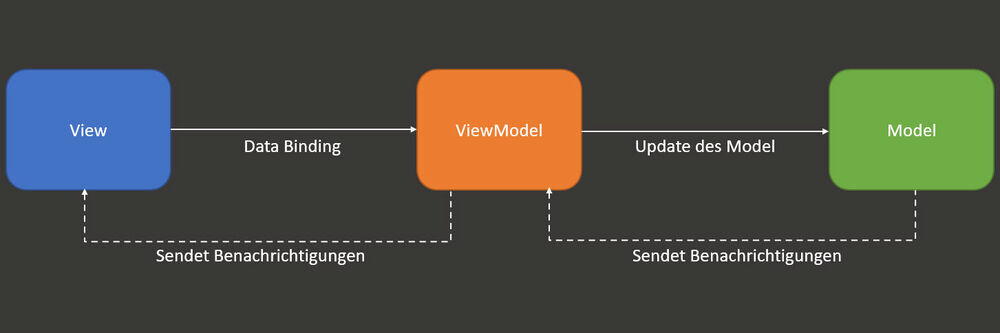
\includegraphics[width=1.0\linewidth]{./images/MVVM.png}
		\caption{MVVM \cite{MVVMKraus}}
		\label{fig:MVVM}
	\end{figure}
	\begin{itemize}
		\item \textbf{Model: } Hier werden Daten aus einer Datenquelle angefordert und bearbeitet.
		\item \textbf{View: } In der View wird die graphische Oberfläche definiert. Zur Darstellung von Daten nutzt sie ViewModel, welches Informationen für die View zur Verfügung stellt.
		\item \textbf{ViewModel: } Das ViewModel ähnelt dem Controller von MVC und stellt die Verbindung zwischen Model und View her. Hier wird die Logik, was bei Änderungen an der Benutzeroberfläche geschehen soll, implementiert. ViewModel holt sich von Model Daten, welche die View für Darstellungszwecke benötigt. \cite{MVVMKraus} \cite{troelsen2022pro}
	\end{itemize}
	Auf die Verbindung wischen den einzelnen Komponenten mit Datenbindung wird im folgenden unter Entwurfsmuster eingegangen.\\
	\textbf{Entwurfsmuster}\\
	Nach Gollar, Koller und Watzko \cite{ArchitekturmusterGoll} bieten sich für die MVC-Architektur und somit auch für die MVVM-Architektur mehrere Entwurfsmuster an. Am geläufigsten ist das Beobachter-Muster (engl. Observer-Pattern). Weitere Entwurfsmuster sind das Strategie-Muster und das Kompositum-Muster \cite{ArchitekturmusterGoll}. Das Beobachter-Muster wird häufig in der Literatur empfohlen und kommt auch in der WPF-Anwendung roboTools umgesetzt durch sogenannte Datenbindung (engl. Data Binding) zum Einsatz. Daher fällt die Entscheidung bei der zu entwerfenden WPF-Anwendung ebenso auf MVVM mit Beobachter-Muster. Die beobachtende Komponente überwacht hierbei eine andere Komponenten. Ändert sich etwas an dem beobachtenden Objekt (wie z.B. ein Tastendruck) erkennt dies der Beobachter und kann in Folge dessen eine definierte Aktion ausführen. \cite{ArchitekturmusterGoll}\\
	Die Verbindung zwischen View und ViewModel, sowie zwischen ViewModel und Model wird mit Hilfe von Datenbindung umgesetzt. Die Datenbindung gibt sozusagen Daten zwischen einzelnen Komponenten weiter.\\
	\textbf{Adaption der Anwendung auf Architektur- und Entwurfsmuster}\\
	Um die Komponenten der zu entwerfenden Software zu definieren, müssen die Anwendungen, die im UML-Diagramm (vgl. Abbildung \ref{fig:UML_Use_Case_WPF}) definiert wurden auf das Entwurfsmuster aufgeteilt werden. Ebenso müssen die Klassen für die zu entwerfende WPF-Anwendung in C\# definiert werden. Gemäß MVVM werden in der View (gemäß unternehmensinternem Standard als "MainWindow" bezeichnet)
	die Grafik des Programms festgelegt. Hier müssen sowohl der Protokollschreiber der Systemereignisse, sowie Diagramme zur Darstellung der Prozessdaten definiert werden. In der View soll jedoch keine Logik umgesetzt und der Code auf ein Minimum begrenzt werden. Im Model hingegen erfolgt gemäß MVVM die Datenhaltung und Datenverarbeitung. Hier werden Daten über die TCP/IP-Verbindung empfangen und gesendet, sowie die Daten abgespeichert. Das ViewModel (unternehmensintern als MainViewModel bezeichnet) verkünpft die View und das Model. So soll auf Knopfdruck in der View, Prozessdaten aus dem Model ausgelesen und in der View dargestellt werden. Die Logik hierfür erfolgt in dem ViewModel (hier: MainViewModel). Für den Entwurf der WPF-Anwendung bietet sich daher folgende Klassenaufteilung an, welche nachfolgend in einem UML-Klassendiagramm dargestellt ist (vgl. Abbildung \ref{fig:UMLKlassenWPF}). Diese Klassen und ihre Funktionen sind in der Umsetzung mit C\# zu implementieren.
	\begin{figure}
		\begin{tikzpicture}
			\begin{umlpackage}{ViewModel}
				\umlclass[name=viewModel, x=0]{MainViewModel}{
				}{
					+ PlotteDaten() : void \\
					+ LeseCSVDatei() : void \\
					+ BefülleAnzeigeVerbundeneRoboter(): void \\
					+ BefülleAnzeigeServerEinstellungen(): void 
					
				}
			\end{umlpackage}
			
			\begin{umlpackage}{View}
				\umlclass[name=view, x=8]{MainWindow}{
					- Graphik: \\
					- Aktualisierungsbutton: \\
					- Anzeige verbundene Roboter: \\
					- Anzeige Servereinstellungen: \\
					- Protokollschreiber:
				}{
					
				}
			\end{umlpackage}
			
			\begin{umlpackage}{Model}
				\umlclass[name=com, x=0, y=-6]{Communicator}{
					- IP-Adresse : float \\
					- Verbundene Clients: Dictionary
				}{
					+ Empfange Nachricht() : void \\
					+ ÜberprüfeErrreichbarkeitRoboter(): void \\
					+ SendeDatenafoderungtelegramm(): void \\
					+ SendeAktualisierungsTelegramm \\SchwereSystemereignis(): void\\
					+ SendePositionsdaten(): void \\
					+ ÜbergebeNachrichtInterpreter(byte[]): void
				}
				
				\umlclass[name=robot, x=8, y=-5]{Robot}{
					- Name: string \\
					- Erreichbarkeit: bool \\
					- Temperatur: int \\
					- Fehler: bool \\
					- Schwere Systemereigniss: int
				}{
					
				}
				\umlclass[name=interpreter, x=7.5, y=-9]{Interpreter}{
					- Nachricht: byte[]
				}{
					+ InterpretiereDatentelegramm(): void \\
					+ SpeichereDaten(): void \\
					+ InterpretiereSystemereignis\\-Telegramm(): void \\
					+ SpeichereSystemereignisse(): void \\
				}
			\end{umlpackage}
			
			
			% Verbindungslienie zwischen SPS und Roboter mit Multiplicitäten
			\umluniassoc[pos=0.5]{MainViewModel}{MainWindow}
			\umluniassoc[pos=0.5]{MainWindow}{MainViewModel}
			
			\umluniassoc[pos=0.5]{MainViewModel}{Communicator}
			\umluniassoc[pos=0.5]{Communicator}{MainViewModel}
			
			\umluniassoc[pos=0.5]{Communicator}{Interpreter}
			\umluniassoc[pos=0.5]{Communicator}{Robot}
			\umluniassoc[pos=0.5]{Interpreter}{Robot}
			
		\end{tikzpicture}
		\caption{UML-Klassendiagramm WPF-Anwendung}
		\label{fig:UMLKlassenWPF}
	\end{figure}
	
	\textbf{Benutzeroberfläche}\\
	Alle Elemente, wie die Ausgabe der Systemereignisse oder die grafische Darstellung der Prozessdaten sollen möglichst übersichtlich dargestellt werden und es sollen möglichst viele Informationen integriert werden. Neben den Daten sollen dem Nutzer Serverinformationen und eine Liste der verbundenen Roboter bereitgestellt werden. Es soll zwischen den einzelnen verbundenen Robotern gewählt werden können für welchen Roboter die Prozessdaten visualisiert werden sollen. Über ein Aktualisierungsknopf werden die Daten aktualisiert dargestellt. Auf eine zyklische automatische Aktualisierung wird verzichtet, um Rechenkapazität einzusparen.\\
	Dadurch, dass die Anwendung später in roboTools integriert wird, ist das visuelle Erscheinungsbild nicht von höchster Bedeutung. Einzelne Elemente, wie z.B. die Ausgabe der Systemereignisse oder die Diagramme mit den Prozessdaten werden in roboTools integriert, wobei das optische Erscheinungsbild, wie z.B. das Unternehmenslogo und die Farbgestaltung durch roboTools bereits vorgegeben ist. Eine Integration ist durch den Einsatz von Datenbindung besonders einfach möglich (vgl. Kapitel \ref{sec:KonzeptWPF}).
	Die Anordnung der einzelnen Elemente ist nachfolgend dargestellt (vgl. Abbildung \ref{fig:WPF_GUI_Nachrichten} und \ref{fig:WPF_GUI_Graph}). Dabei erfolgt eine Trennung der Protokoll-Ausgaben und der Graphen in zwei verschiedene Registerkarten. \\
	\begin{figure}
		\begin{tikzpicture}
			% Großes Rechteck mit der Breite des Textes
			\draw (0,0) rectangle (\textwidth, 9);
			
			% Kleine Rechtecke mit Text
			% Kleine Rechtecke mit Text
			\draw (0.2 , 0.2) rectangle ++(14,2.5) node[pos=.5] {Systemereignisse};
			\draw (0.2 , 2.9) rectangle ++(14,2.5) node[pos=.5] {Protokoll der WPF-Anwendung};
			\draw (0.2, 5.6) rectangle ++(9,2.5) node[pos=.5] {Prozessdaten};
			\draw (10.2, 7.3) rectangle ++(4,1.5) node[pos=.5] {Serverinformation}; 
			\draw (10.2, 5.6) rectangle ++(4,1.5) node[pos=.5] {Verbundene Roboter}; 
			\draw [fill=lightgray] (0.2, 8.5) rectangle ++(2.5,0.5) node[pos=.5] {Nachrichten}; % Reiter 1
			\draw (2.7, 8.5) rectangle ++(2,0.5) node[pos=.5] {Graph}; % Reiter 2
			
		\end{tikzpicture}
		\caption{WPF-Anwendung Benutzeroberfläche Registerkarte Nachrichten}
		\label{fig:WPF_GUI_Nachrichten}
	\end{figure}
	
	\begin{figure}
		\begin{tikzpicture}
			% Großes Rechteck mit der Breite des Textes
			\draw (0,0) rectangle (\textwidth, 9);
			
			% Kleine Rechtecke mit Text
			% Kleine Rechtecke mit Text
			\draw (0.2 , 3.4) rectangle ++(4.6,3) node[pos=.5] {Diagramm 1};
			\draw (5.0 , 3.4) rectangle ++(4.6,3) node[pos=.5] {Diagramm 2};
			\draw (9.8 , 3.4) rectangle ++(4.6,3) node[pos=.5] {Diagramm 3};
			
			\draw (0.2 , 0.2) rectangle ++(4.6,3) node[pos=.5] {Diagramm 4};
			\draw (5.0 , 0.2) rectangle ++(4.6,3) node[pos=.5] {Diagramm 5};
			\draw (9.8 , 0.2) rectangle ++(4.6,3) node[pos=.5] {Diagramm 6};
			
			\draw (0.2, 7) rectangle ++(3,1) node[pos=.5] {Aktualisiere}; 
			\draw (3.4, 7) rectangle ++(4,1) node[pos=.5] {Auswahl Roboter}; % ggf. \blacktriangledown
			\draw (7.6, 7) rectangle ++(5,1) node[pos=.5] {Letzte Aktualisierung};
			
			\draw (0.2, 8.5) rectangle ++(2.5,0.5) node[pos=.5] {Nachrichten}; % Reiter 1
			\draw [fill=lightgray] (2.7, 8.5) rectangle ++(2,0.5) node[pos=.5] {Graph}; % Reiter 2
			
		\end{tikzpicture}
		\caption{WPF-Anwendung Benutzeroberfläche Registerkarte Graph}
		\label{fig:WPF_GUI_Graph}
	\end{figure}
	
	Hierbei wurde versucht alle Informationen zu integrieren. Beispielhaft ist die Protokollierung des Programmablaufes enthalten, auch wenn eine Integration dieser Ausgabe für den Endnutzer in roboTools nicht vorgesehen ist, sondern lediglich eine lokale Speicherung. Zu Debugging-Zwecken oder zur Fehlerfindung an dem Roboter bei Reparaturarbeiten ist eine Ausgabe aller Daten jedoch hilfreich.
	
	
	\chapter{Design und Implementierung}
	Im Rahmen dieses Kapitels soll das Design der Software erfolgen. Lösungsbausteine, wie z.B. Softwarebibliotheken müssen festgelegt und Lösungsansätze entworfen werden. Darüber hinaus, erfolgt die Implementierung durch Source-Code. Im Rahmen dieser Arbeit werden nur einzelne besonders relevante Segmente des Codes aufgezeigt. Dies erfolgt getrennt für das Roboterprogramm in VAL 3 und die WPF-Anwendung.
	\section{Stäubli-Roboter in VAL 3}
	
	\subsection{EtherCAT}
	Nachdem die Feldbus-Verbindung in Kapitel \ref{sec:KonzeptFeldbus} konzeptioniert wurde, wird nachfolgend die Umsetzung der gewählten Konfiguration der Feldbus-Verbindung kurz erläutert.\\
	Um eine EtherCAT Verbindung zwischen der SPS und der Stäubli Steuerung CS9 herzustellen muss zuerst eine physische Verbindung geschaffen werden. Ein LAN-Kabel verbindet den Master SPS mit dem Slave CS9. Anschließend erfolgt eine Konfiguration der EtherCAT-Verbindung in der \acl{srs}. Hierzu dient eine in die SRS integrierte Anwendung namens \glqq SYCON.net \grqq{} des Anbieters \glqq Hilscher GmbH \grqq. Hier wird unter anderem die zu übertragende Datenmenge festgelegt. Dabei erfolgt eine detaillierte Festlegung der zu übertragenden digitalen und analogen Werte. Es werden die zu übertragenden Daten, sowie deren Größe (z.B. 1 Byte oder ein Word, welches sich aus 2 Byte zusammensetzt) festgelegt. Von der Feldbus-Konfiguration kann eine sogenannte ESI-Datei erzeugt werden, welche in die SPS geladen wird, damit diese die EtherCAT-Konfiguration kennt. Nach der erfolgreichen Konfiguration muss in VAL~3 auf die EtherCAT-Verbindung zugegriffen werden, um Werte zu lesen oder zu beschreiben. Hierzu werden die einzelnen Daten der EtherCAT-Nachricht mit Variablen in der E/A-Verwaltung verknüpft. \cite{CS9} \cite{CS9_Fieldbus}\\
	Beispielsweise kann eine von der SPS gesendete Auftragsnummer über den Befehl \glqq aioGet\grqq{} gelesen werden. Je nach Auftragsnummer wird ein gewisser Bewegungsablauf ausgeführt.
	\begin{lstlisting}
		// Abfrage der Auftragsnummer von der EtherCAT-Schnittstelle
		jobNumber = aioGet(aiJobNumber)
		switch jobNumber
		case 4
			// Aufruf zur Bewegungsausführung
			call moveToHome()
		break
	\end{lstlisting}
	Ebenso können erfolgreich durchgeführte Bewegungen mit dem Befehl \glqq aioSet\grqq{} bestätigt werden, in dem eine Übergabe an die EtherCAT-Verbindung erfolgt. \cite{VAL3} 
	
	\subsection{TCP/IP}
	Nach erfolgreicher Implementierung der EtherCAT-Verbindung soll die TCP/IP-Verbindung implementiert werden. Dabei sollen die in Kapitel \ref{sec:KonzeptTCPIP} getroffenen Entscheidungen zur TCP/IP-Verbindung  und dem Nachrichtenaufbau, wie dort konzeptioniert umgesetzt werden. Ebenso soll das Roboterprogramm in VAL~3 gemäß Kapitel \ref{sec:KonzeptVAL3} umgesetzt werden. Dies beinhaltet das Programm Empfangen, in welchem beispielsweise Datenanforderungstelegramme empfangen werden und mit einem Datentelegramm beantwortet werden. Ebenso sind die Programme zum Versand der Systemereignisse und zur Bewegungsausführung und Motormoment-Berechnung zu implementieren. Der Programmcode in VAL~3 wird hierbei nicht komplett aufgezeigt, sondern lediglich das Grundprinzip, sowie Besonderheiten aufgezeigt.\\
	\textbf{Implementierung TCP/IP-Verbindung}\\
	Für die Implementierung der TCP/IP-Verbindung auf dem Controller des Stäubli-Roboters muss in der SRS eine Socket-Verbindung angelegt werden. Hierzu wird in der E/A-Verwaltung ein Client angelegt, welcher die IP-Adresse und den Port des Servers zugewiesen bekommt. Darüber hinaus wird ein sogenannter Timeout von 0 s gesetzt. Bei einem Timeout von 0 wird auf den Vorgang, welcher ein Lesen oder Schreiben sein kann gewartet. Bei einem Timeout kleiner 0 wird hingegen nicht bis zur Ausführung des Vorgangs gewartet. Bei einem Timeout größer 0 wird hingegen eine gewisse Zeit gewährt, bis zu dieser der Timeout durchgeführt werden kann. Die Nachricht soll in diesem Fall jedoch direkt gelesen oder geschrieben werden, weshalb kein Spielraum im Rahmen des Timeouts gewährt wird. \cite{VAL3} Die Socket-Verbindung wird als E/A-Verbindung in VAL3 betrachtet, weshalb eine globale Variable mit dem Namen des Clients angelegt werden kann und hierüber auch gelesen und beschrieben werden kann. Die Socket-Verbindung wird nur dann erstellt, wenn sie ihm Rahmen des Programmablaufs z.B. durch die Befehle sioSet und sioGet benötigt wird. Der Client versucht dann eine Verbindung zum Server aufzubauen. \cite{VAL3} \cite{CS9_TCP}\\
	\textbf{Empfangen}\\
	In diesem Programm müssen zu Beginn eingehende Nachrichten der TCP/IP-Verbindung gelesen werden. Dies erfolgt mit folgendem Befehl:
	\begin{lstlisting}
		l_nResult=sioGet(sio_client,nReceive)
	\end{lstlisting}
	Diese Funktion schreibt ein gelesenes Zeichen oder einen gelesen Array von Zeichen von sio\_client in das Array nReceive. Als Rückgabewert dient die Anzahl der gelesenen Zeichen. Nachfolgend können die einzelnen Bytes der Nachricht interpretiert werden und somit entschieden werden, ob es sich um ein Datenanforderungstelegramm, eine Aktualisierung der Systemereignis-Schwere oder Positionsdaten handelt. \cite{VAL3} \cite{CS9_TCP}\\
	Im Falle eines Datenanforderungstelegramm muss ein Datentelegramm gemäß der Konzeptionierung des Datentelegramms (vgl. Kapitel \ref{sec:KonzeptTCPIP})) aufgebaut werden. Hierzu werden beispielsweise Temperaturen der Antriebe von den E/A-Boards der CS9 ausgelesen. Diese eingelesenen numerischen Daten können durch folgenden Befehl in einen Byte-Strom gewandelt werden:
	\begin{lstlisting}
		num toBinary(nValue[], nValueSize, sDataFormat, nDataByte[])
	\end{lstlisting}
	Diese Funktion wandelt einen numerischen Wert, welcher das Datenformat sDataFormat besitzt in einen Byte-Strom und speichert diesen im Array nDataByte. Über das Datenformat wird beispielsweise angegeben ob es sich um einen Gleitkommawert handelt, ob ein Vorzeichen vorliegt und ob das Little-Endian oder das Big-Endian-Format angewandt wird. Mit nDataSize kann die Anzahl der zu kodierenden Zeichen beschränkt werden.\\
	Anschließend werden die gewandelten Bytes in den Byte-Array des zusendeten Datentelegramms geschrieben. Das fertige Datentelegramm wird anschließend über folgenden Befehl versendet \cite{VAL3}:
	\begin{lstlisting}
		l_nResult=sioSet(sio_client,nSendMessage)
	\end{lstlisting}
	Mit dieser Funktion kann in VAL~3 die zu übermittelnde Nachricht nSendMessage versendet werden, indem der E/A-Verbindung sio\_client die Nachricht zugewiesen wird. Zurückgegeben wird die Anzahl der geschriebenen Zeichen oder \glqq -1\grqq{} im Falle des Timeouts. \\
	Handelt es sich anstelle des Datenanforderungstelegramm um ein Telegramm zur Aktualisierung der zu übertragenden Systemereignis-Schwere, wird eine globale Variable, welche die zu übertragende Schwere des Roboters repräsentiert überschrieben. \cite{VAL3} \cite{CS9_TCP}\\
	\textbf{Systemereignisse}\\
	Um die Systemereignisse über TCP/IP an die Anlagenvisualisierung übertragen zu können müssen diese erst ausgelesen werden. Hierzu gibt es in VAL~3 zwei Möglichkeiten. Die eine Funktion ermöglicht die Ausgabe des gesamten Systemereignisses in ausformulierter Textform, die andere wiederum ermittelt nur den Ereigniscode. \cite{VAL3} Diese beiden Funktionen werden nachfolgend in einer Vergleichstabelle mit Hilfe von Harvey Balls verglichen (vgl. Tabelle \ref{tab:getEvent-vergleich}). Der Füllheitsgrad des Harvey Balls entspricht dabei dem Grad der Zielerreichung.
	\begin{table}[h]
		\centering
		\caption{Vergleich Funktion zur Ermittelung Systemereignis}
		\label{tab:getEvent-vergleich}
		\begin{tabularx}{\linewidth}{p{0.2\linewidth} >{\centering\arraybackslash}X >{\centering\arraybackslash}X >{\centering\arraybackslash}X}
			\hline
			\textbf{ } & \textbf{Ausformuliert} & \textbf{Ereigniscode}\\
			\hline
			Datensparend & \harveyBallQuarter& \harveyBallFull\\
			Verständlichkeit/Einfachheit & \harveyBallThreeQuarter & \harveyBallQuarter\\
			Flexibilität & \harveyBallThreeQuarter & \harveyBallQuarter \\
			\hline
		\end{tabularx}
		\begin{flushleft}
			\textbf{Legende:} \harveyBallFull: Hervorragend   \harveyBallHalf: Teils/Teils	\harveyBallNone: Sehr schlecht
		\end{flushleft}
	\end{table}
	Für den Einsatz des Ereigniscodes spricht, dass der Umfang der zu übertragenden Daten viel geringer ist. Dafür muss bei dem Empfänger, der Anlagenvisualisierung, die Bedeutung der jeweiligen Ereigniscodes hinterlegt werden. Dies geht mit einem deutlichen Mehraufwand einher, vergrößert das Programm und reduziert die Verständlichkeit. Ebenso wird die Flexibilität deutlich reduziert, da bei Änderung der Ereigniscodes z.B. durch ein Software-Update oder eine Neubeschaffung des Stäubli-Roboters, eine manuelle Anpassung der Interpretation der Ereigniscodes erfolgen muss. Aus diesem Grund fällt die Entscheidung auf die Übertragung des Systemereignisses in ausformuliert Form.
	Hierzu kommt folgender VAL~3 spezifische Befehle zum Einsatz:
	\begin{lstlisting}
		l_nLastEvt=getEvents(l_nFirstEvt, l_nId, l_nType, l_sInfo, l_nSeverity)
	\end{lstlisting}
	Dieser ermittelt neben dem Systemereignis selbst und der Schwere, eine CS9-interne Nummer des letzten tatsächlich ausgelesenen Ereignisses (l\_nLastEvt).
	Bei der nächsten zyklischen Abfrage der Systemereignisses wird die Nummer des letzten ausgelesenen Ereignisses als Eingangsparameter für das erste auszulesende Ereignis (l\_nFirstEvt) verwendet. Dadurch wird vermieden, dass keine Systemereignisse mehrfach ausgelesen werden. Diese Funktion speichert zudem in l\_nFirstEvt die Nummer des tatsächlich zuerst ausgelesenen Ereignisses. Das System behält nur die letzten 20 Ereignisse gespeichert. Aus der Differenz des tatsächlich ersten ausgelesenen Ereignisses zur der Vorgabe des ersten auszulesenden Ereignisses, lässt sich berechnen ob alle Ereignisse ausgelesen wurden oder ob aufgrund einer Überschreitung der Grenze von 20 Ereignissen, Ereignisse verloren gegangen sind. Die zyklische Abfrage der Ereignisse ist jedoch so dicht getaktet, dass ein Verlorengehen von Ereignissen im Betrieb quasi nicht auftreten kann.\\
	Nach dem Auslesen der Systemereignisse werden diese einzeln als Nachrichten über TCP/IP versendet. Hierbei wird der entworfene Telegrammaufbau von Kapitel \ref{sec:KonzeptFeldbus}) angewandt.\\
	\textbf{Bewegungssteuerung}\\
	In dem Programm Bewegungssteuerung erfolgt die Steuerung der Roboterbewegung. Hierzu werden Punkte in der SRS angelegt, welche durch Teachen an dem realen Roboter auf die genaue geometrische Situation angepasst werden. Nachfolgend ist eine Verfahrbewegung exemplarisch aufgezeigt:
	\begin{lstlisting}
		movel(pZwischenPos, tTool, mLspeed)
	\end{lstlisting}
	Hierdurch erfolgt eine lineare Bewegung zu dem Punkt \glqq pZwischenPos \grqq{}. Die Bewegungsdaten wie Geschwindigkeit und Beschleunigung sind in \glqq mLspeed \grqq{} abgespeichert. Die Geometrie des Robotergreifers ist in der Variablen \glqq tTool \grqq{} hinterlegt.\\
	Zu Beginn einer Bewegungsausführung wird zudem ein neuer Task gestartet, in dem das Drehmoment über die Zeit integriert werden soll. Nach Ablauf des kompletten Bewegungsablauf wird dieser Task wieder beendet. Das aktuelle Ergebnis der Integration wird abgefragt und entspricht dem integrierten Moment eines kompletten Bewegungsablaufes.\\
	\textbf{Motormoment-Integrator}\\
	Dieses Programm, welches von dem Programm Bewegungssteuerung gestartet und beendet wird führt die Integration der Motormomente aller sechs Achsen über die Zeit durch. Mit dem Aufruf des Programms wird das integrierte Motormoment auf Null gesetzt, da es sich um den Beginn eines Bewegungsablaufes handelt. Die Integration wird durch das Bilden einer Summe mit einer Abtastperiode von 0,1 Sekunden realisiert. Dieser Zusammenhang ist in nachfolgender Formel dargestellt:
	\begin{equation}
		\int_{0}^{T} M(t) \, dt \approx \sum_{i=0}^{n} 0,1 \cdot M_i
	\end{equation}
	In einer Endlos-Schleife mit einer Wartezeit von 0,1 Sekunden wird jeweils der Absolutwert des aktuellen Motor-Momentes multipliziert mit 0,1 Sekunden zu dem aktuellen integrierten Motormoment addiert. Das aktuelle integrierte Motormoment kann am Ende eines Bewegungsablaufes abgefragt werden und entspricht somit dem integrierten Motormoment über die Zeit des gesamten Bewegungsablaufes.
	\section{WPF-Anwendung}
	Wie in Stand der Technik (vgl. Kapitel \ref{sec:WPF}) analysiert, soll für die Implementierung der WPF-Anwendung C\# zum Einsatz kommen. Als Entwicklungsumgebung dient Visual Studio und als Source-Code-Verwaltungs-Programm wird \glqq Azure DevOps\grqq{} eingesetzt. In Kapitel \ref{sec:KonzeptWPF} wurde MVVM als Architekturmuster gewählt. Mit Hilfe eines Klassendiagramms wurde festgelegt, dass neben den Klassen MainWindow und MainViewModel, die Klassen Communicator, Robot und Interpreter, welche zusammen das Model bilden, existieren sollen. Im Klassendiagramm wurden zudem die Methoden der jeweiligen Klassen definiert. Auf eine detailreiche Darstellung der Implementierung wird in diesem Kapitel verzichtet. Stattdessen werden richtungsweisende Entscheidungen, sowie Grundprinzipien und wichtige Funktionen erläutert.
   	\subsection{TCP/IP-Server}
   	In der Klasse Communicator muss ein TCP/IP-Server umgesetzt werden, der zudem Nachrichten sendet und empfängt.
   	Hierzu wird in einem ersten Schritt eine Instanz der Klasse TcpListener unter Angabe der IP-Adresse und des Ports erstellt. \cite{MicrosoftTCP}\\
   	\begin{lstlisting}
   		tcpListener = new TcpListener(localAddr, port);
   	\end{lstlisting}
   	Nachdem der Server erstellt wird muss auf Clients gewartet werden, die sich verbinden möchten. Dies wird in einer Endlos-Schleife realisiert, die nur durch ein Schließen des Programmes gesteuert unterbrochen wird. Dies ermöglicht es, dass mehrere Clients eine Verbindung zu dem Server aufbauen können. Ebenso erhält ein Client, der eine Verbindung abgebrochen hat, die Chance eine erneute Verbindung aufzubauen. Der Verbindungsaufbau wird durch folgenden Befehl realisiert:
   	\begin{lstlisting}
   		var tcpClient = await tcpListener.AcceptTcpClientAsync();
   	\end{lstlisting}
   	Nachfolgend wird noch innerhalb der endlos-Schleife eine asynchrone Methode aufgerufen, die es ermöglicht Nachrichten von der Verbindung zu lesen.
   	Bei Aufruf der asynchronen Methode, wird nicht auf das Ende der Methode gewartet, sondern die Ausführung wird direkt nach Aufruf fortgeführt \cite{kotz2022c}. Dies ermöglicht es in einem erneuten Schleifen-Durchlauf direkt eine Verbindung zu einem neuen Client aufzubauen. Das Prinzip der asynchronen Methoden ermöglicht daher, eine Kommunikation mit mehreren Robotern sicherzustellen, was einer Kann-Forderung aus dem Lastenheft entspricht. Zudem kann diese Methode mehrfach gleichzeitig für jeden einzelnen Client ausgeführt werden. Bei Aufruf der asynchronen Methode muss der zuvor verbundene Client übergeben werden.
   	Innerhalb dieser Methode wird ein sogenannter Netzwerkstream aufgerufen und als Objekt zurückgegeben.
   	\begin{lstlisting}
   		var stream = client.GetStream();
   	\end{lstlisting}
   	Netzwerkstream ist eine Klasse in .NET und stellt Methoden zum Senden und Empfangen von Nachrichten.
   	Nachfolgend wird über die Methode ReadAsync der Klasse NetworkStream von dem Netzwerkstream gelesen und in einen Byte-Array namens bufferIn geschrieben.
   	\begin{lstlisting}
   		int bytesRead = await stream.ReadAsync(bufferIn, 0, bufferIn.Length);
   	\end{lstlisting}
   	Der await-Operator ermöglicht es, dass das Ende dieser Methode (ReadAsync) trotz des asynchronen Charakters abgewartet wird \cite{kotz2022c}.\\
   	\textbf{Nachrichteninterpretation} \\
    Anschließend muss der gelesene Byte-Array interpretiert werden. Hierfür wird gemäß der Konzeptionierung der WPF-Anwendung (vgl. Kapitel \ref{sec:KonzeptWPF}) eine eigene Klasse namens Interpreter erstellt. Nach dem Lesen einer TCP-IP Nachricht kann eine Methode dieser Klasse entweder ein Datentelegramm oder ein Systemereignis-Telegramm entschlüsseln bzw. interpretieren, in dem dieser Methode der Byte-Array übergeben wird. Dort werden dann die einzelnen Bytes der Nachricht gelesen und somit z.B. die Temperatur der CPU ermittelt. Diese ermittelten Eigenschaften werden in eine Instanz der Klasse Robot, welche somit einen einzelnen konkreten Roboter darstellt, geschrieben.\\
    \textbf{Verbundene Roboter} \\
    Zusätzlich soll die Klasse Communicator ermitteln, welche Roboter aktuell eine Verbindung mit dem Server aufgebaut haben. Diese Information kann über das Fenster, dem Nutzer angezeigt werden. Die Schwierigkeit besteht darin, dass über die aufgebauten Verbindungen zwar einfach dokumentiert werden kann, ob Clients verbunden sind, jedoch keine Information darüber besteht, um welchen Roboter es sich dabei handelt. Die Identifikation des Roboters kann erst mit der ersten Nachricht des Roboters erfolgen, in welcher der Robotername enthalten ist. Zur Speicherung der verbunden Clients und den damit verknüpften Robotern ergeben sich mehrere Möglichkeiten. Beispielsweise kann eine Liste von Tupeln angelegt werden, als Schlüssel kann der Client dienen und als Wert der Roboter. Eine andere Alternative stellt eine Liste oder ein Array aus benutzerdefinierten Objekten dar. Das Objekt besteht in diesem Fall aus dem Client und dem Roboter. Eine weitere Möglichkeit ist ein Dictionary. Dies ermöglicht es Mengen von Schlüssel-Werte-Paaren zu speichern.
    Gegen den Einsatzes einer Liste mit Objekten spricht, dass dies den Aufwand und die Komplexität erhöht, da diese Objekte erst kreiert werden müssen.
    Die Besonderheit von Listen mit Tupeln hingegen ist, dass die Elemente in einer vorgegeben Sequenz angeordnet sind und ein Zugriff über die Reihenfolge erfolgen kann. In diesem Anwendungsfall ist die Sequenz der Elemente jedoch ohne Bedeuutung, weshalb sich ein Dictionary besonders für die Anwendung eignet. Dieses ermöglicht einen effizienten Zugriff mit Hilfe der schlüsselbasierten Suche. \cite{troelsen2022pro} \cite{kotz2022c}
    Die Initialisierung des Dictionarys ist nachfolgend dargestellt.
    \begin{lstlisting}
    	private ConcurrentDictionary<TcpClient, Robot> dictionaryConnectedClients = new ConcurrentDictionary<TcpClient, Robot>();
    \end{lstlisting}
    Der TcpClient wird in diesem Fall als Schlüssel eingesetzt und das Objekt der Klasse Robot dient als Wert. Ein ConcurrentDictionary unterscheidet sich von einem normalen Dictionary durch seine Fähigkeit, sicher von mehreren Threads gleichzeitig bearbeitet zu werden, ohne dass externe Synchronisierung notwendig ist. Da mehrere Clients verbunden sein können, kann es dazukommen, dass mehrere asynchronen Methoden zeitgleich das Dictionary beschreiben möchten.
   	Wird erstmalig eine Verbindung zu einem Client aufgebaut wird dieser in das Dictionary aufgenommen, bricht eine Verbindung ab, wird dieser wieder aus dem Dictionary entfernt. Wird erstmalig ein Roboter durch seinen Namen identifiziert, wird dieser dem entsprechenden Client als Wert im Dictionary zugewiesen.\\
   	\textbf{Konfigurationsdatei}\\
   	Darüberhinaus ist eine Konfigurationsdatei in die WPF-Anwendung implementiert, in der wichtige Einstellungen von dem Betreiber hinterlegt werden. Hier wird z.B. neben der IP-Adresse und des Ports, eine Liste der installierten Roboter abgelegt. Durch ein Vergleich dieser mit den tatsächlich verbundenen Robotern im Dictionary, kann eine Warnung ausgegeben werden, dass ein gewisser Roboter nicht verbunden ist. Zudem ist in dieser Datei hinterlegt, ab welcher Schwere Systemereignisse übertragen werden sollen. Gemäß Konzeptionierung der WPF-Anwendung (vgl. Kapitel \ref{sec:KonzeptWPF}) muss die WPF-Anwendung den Robotern mitteilen, ab welcher Schwere diese die Systemereignisse versenden sollen. Wird erstmalig eine Verbindung zu einem Roboter aufgebaut oder nach einem Abbruch der Verbindung erfolgt ein erneuter Aufbau, wird ein Telegramm an diesen Roboter versandt, welches diese Soll-Schwere enthält. Liegt beispielsweise eine Störung oder Auffälligkeit an einem Roboter vor kann ein Servicetechniker die Konfigurationsdatei anpassen (ggf. auch per Fernzugriff) und es dadurch ermöglichen, dass alle Systemereignisse, wie z.B. auch reine Informationen übertragen werden.
   	\subsection{Daten-Logger}
   	Um die Prozessdaten, vor allem aber die Systemereignisse zu protokollieren gibt es mehrere Möglichkeiten. Einerseits kann eine entsprechende Funktion selbst implementiert werden, alternativ kann auf eine Logging-Bibliothek zurückgegriffen werden. Hierfür existieren eine Vielzahl an verschiedenen Anbieter von NLog bis hin zu ELMAH. \cite{logging} Einige Lösungen werden nachfolgend kurz vorgestellt
   	\begin{itemize}
   		\item \textbf{NLog:} Diese Logging-Bilbiothek zählt zu den weit verbreitetsten und performantesten Lösungen. Es ermöglicht ebenso lokale Logging-Files zu erzeugen. Dieses Framework wurde bereits in der Vergangenheit bei robomotion eingesetzt. NLog steht kostenfrei zur Verfügung.
   		\item \textbf{Log4NET:} Der Aufbau und der Funktionsumfang ähnelt stark NLog und es erhebt ebenso keine Lizenzkosten.
   		\item  \textbf{ELMAH:} Diese Bibliothek ist spezialisiert auf das Protokollieren von Fehlern. Es erhebt keine Gebühren. \cite{logging}
   	\end{itemize}
   	Die vorgestellten Lösung einschließlich einer manuellen Implementierung werden nachfolgend gegenübergestellt (vgl. Tabelle \ref{tab:Logger}).
   	\begin{table}[h]
   		\centering
   		\caption{Vergleich Logging-Möglichkeiten}
   		\label{tab:Logger}
   		\begin{tabularx}{\linewidth}{p{0.2\linewidth} >{\centering\arraybackslash}X >{\centering\arraybackslash}X >{\centering\arraybackslash}X >{\centering\arraybackslash}X >{\centering\arraybackslash}X}
   			\hline
   			\textbf{ }  & \textbf{NLog} & \textbf{Log4NET} &   \textbf{ELMAH} & \textbf{Manuell}\\
   			\hline
   			Umfang & \harveyBallThreeQuarter& \harveyBallThreeQuarter& \harveyBallHalf& \harveyBallFull\\
   			Implementierungs-freundlichkeit & \harveyBallThreeQuarter & \harveyBallHalf & \harveyBallHalf & \harveyBallNone\\
   			Standardisierung & \harveyBallThreeQuarter & \harveyBallNone & \harveyBallNone  & \harveyBallNone \\
   			Kostengünstig & \harveyBallFull & \harveyBallFull & \harveyBallFull & \harveyBallFull \\
   			\hline
   		\end{tabularx}
   		\begin{flushleft}
   			\textbf{Legende:} \harveyBallFull: Hervorragend   \harveyBallHalf: Teils/Teils	\harveyBallNone: Sehr schlecht
   		\end{flushleft}
   	\end{table}
   	Der Funktionsumfang ist bei der manuellen Lösungen am höchsten zu bewerten, da jede beliebige Funktion implementiert werden können. ELMAH hingegen ist etwas spezialisierter als NLog und Log4NET, weshalb hier der Funktionsumfang etwas geringer ausfällt. Bei der Implementierungsfreundlichkeit sind die Bibliotheken klar der manuellen Lösung überlegen. NLog stellt hier die einfachste Lösung dar, da bei Bedarf auf die vorherige Erfahrung aus früheren Projekten zurückgegriffen werden kann. Ebenso ist bei NLog die Standardisierung am höchsten einzustufen, da es bereits in anderen Anwendungen zum Einsatz kommt. Alle vier Möglichkeiten sind zudem kostenfrei, weshalb alle die maximal mögliche Wertung erhalten. Die Gesamtentscheidung fällt auf Basis der vorangegangenen Punkten klar auf NLog.
   	Bei der Implementierung von NLog kann zudem ein lokaler Ablageort als sogenanntes TargetFile angegeben werden. Dies ermöglicht es, die Systemereignisse und die Prozessdaten als CSV- bzw. Text-Datei abzuspeichern. Ebenso ist es möglich eine Ausgabe durch einen sogenannten NlogViewer zu realisieren. Dadurch kann eine Darstellung für den Nutzer erfolgen. Zum Einsatz kommt die \glqq Sentinel.NLogViewer \grqq{}-Bibliothek.\\
   	NLog bietet verschiedene \glqq Logging-Levels \grqq{} wie z.B. Info oder Fatal an \cite{nlog}. Bei den übertragenen Systemereignissen wird die Schwere in der Nachricht übertragen. Nach Interpretation dieser Schwere, kann das Systemereignis über NLog mit dem selben Level ausgegeben werden, wie nachfolgend exemplarisch dargestellt ist:
   	\begin{lstlisting}
   		_EventLogger.Error(senderName + ": " + messageContent);
   	\end{lstlisting}
   	Es werden drei verschiedene Logger-Instanzen angelegt. Eine für das Protokollieren von Systemereignissen, eine für die Prozessdaten und eine für den Ablauf der WPF-Anwendung, z.B. für wichtige Ereignisse oder Fehler.

   	\subsection{Diagramm}
   	Die erfassten und gespeicherten Prozessdaten, wie z.B. die Temperatur der CPU soll als graphischer Verlauf über die Zeit dargestellt werden. Für die Erstellung von Diagrammen gibt es in C\# eine Vielzahl von Bibliotheken. Bekannte Bibliotheken sind Oxyplot, LiveCharts und ScottPlot. Aufgrund des besonders positiven optischen Erscheines von OxyPlot fällt die Wahl auf diese Bibliothek. Zudem sind die Anpassungsmöglichkeiten bei LiveCharts und ScottPlot geringer. Prinzipiell lässt sich für die Umsetzung jedoch jede Bibliothek einsetzen. Für das Erstellen eines Diagrammes mit OxyPlot müssen in einem ersten Schritt die Prozessdaten aus der CSV-Datei gelesen und in einer Liste von Tuples abgespeichert werden. Für die Darstellung der x-Achse dient die Uhrzeit, für die y-Achse der eigentliche Datenwert. Abschließend wird ein Diagramm dieser Daten mit Hilfe von OxyPlot erstellt. Darüberhinaus wird realisiert, dass es möglich ist mehrere Daten, wie z.B. die Temperaturen verschiedener Achsen in einem Diagramm darzustellen. Hierzu werden mehrere Spalten aus der CSV-Datei ausgelesen und für die einzelnen Datenreihen verwendet. Eine Legende mit einer Beschriftung der Datenreihen komplettiert das Diagramm. \\
   	Da eine Vielzahl von Robotern in einer Anlage eingesetzt werden, wird ein Dropdown-Menü angelegt, um zwischen den einzelnen Robotern in der Darstellung wechseln zu können. Das Dropdown-Menü bezieht die Roboternamen automatisiert aus der appsettings.json-Datei, in der alle installierten Roboter hinterlegt sind. Es wird bewusst diese Liste und nicht das Dictionary der tatsächlich verbundenen Roboter als Basis für das DropDown-Menü verwendet. Dadurch ist es auch noch nach Ausschalten eines Roboters und eines einhergehenden Verbindungsabbruch möglich, Daten dieses Roboters aus der CSV-Datei darzustellen. Die Diagramme werden bei Programmstart einmalig automatisiert erstellt, ebenso wie bei einer Neuauswahl im DropDown-Menü. Jedoch werden sie nicht zyklisch automatisiert aktualisiert, um Rechenkapazität zu sparen und da sich die Daten meist nicht hochdynamisch ändern. Ein Aktualisierungsschalt-Feld erlaubt ein nachträgliches Aktualisieren.
   	\begin{figure}[!ht]
   		\centering
   		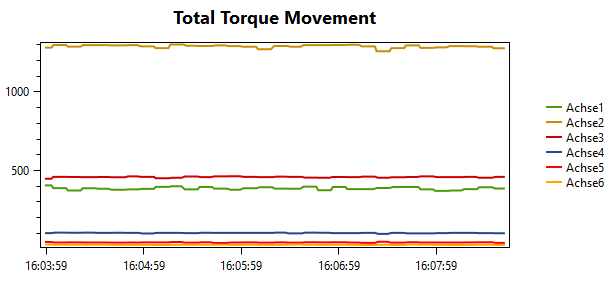
\includegraphics[width=1.0\linewidth]{./images/Diagrammoxyplot.png}
   		\caption{OxyPlot - Diagramm}
   		\label{fig:oxyplot}
   	\end{figure}
   	
   	\subsection{Benutzeroberfläche}
   	Für die Darstellung der gesammelten Informationen, wie die Systemereignisse oder die Prozessdaten in Diagrammform muss eine Benutzeroberfläche implementiert werden. Gemäß gewähltem MVVM-Muster (vgl. Kapitel \ref{sec:KonzeptWPF}) erfolgt die Definition der Benutzeroberfläche in der Klasse MainWindow. Mittels XAML werden einzelne Elemente, wie z.B. Buttons oder OxyPlot-Diagramme angelegt und mittels DatenBindung mit der Klasse MainViewModel verknüpft.\\
   	Der Aufbau der Benutzeroberfläche erfolgt gemäß der grafischen Anordnung aus der Konzeptionierung der WPF-Anwendung. Das Ergebis ist unterteilt in die Registerkarte \glqq Nachrichten\grqq{} (vgl. Abbildung \ref{fig:TabLogger}) und \glqq Graph\grqq{} (vgl. Abbildung \ref{fig:TabGraph}) nachfolgend dargestellt.\\
   	\begin{figure}[!ht]
   		\centering
   		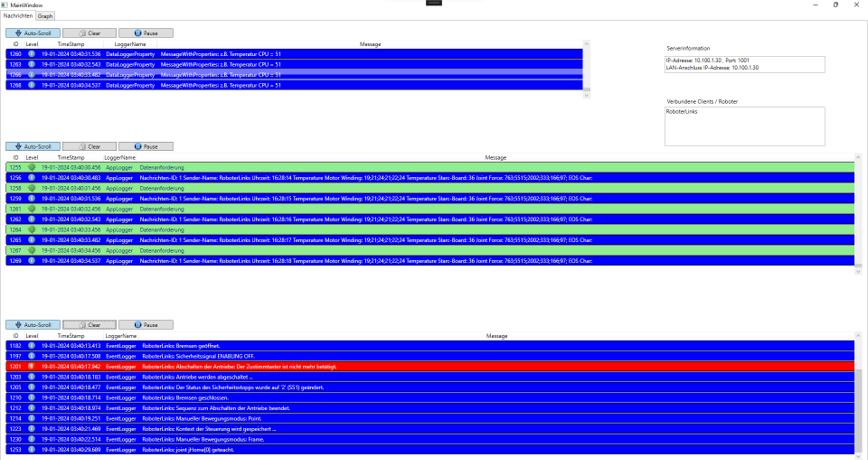
\includegraphics[width=1\linewidth]{./images/TabLogger.png}
   		\caption{Benutzeroberfläche Registerkarte Nachrichten}
   		\label{fig:TabLogger}
   	\end{figure}\\
   	\begin{figure}[!ht]
   	\centering
   	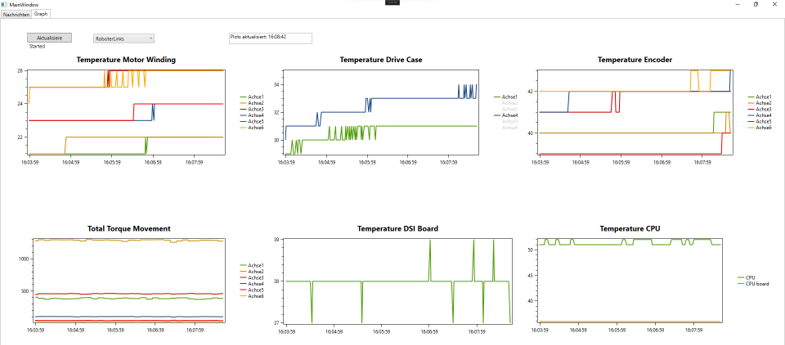
\includegraphics[width=1\linewidth]{./images/TabPlot.png}
   	\caption{Benutzeroberfläche Registerkarte Graph}
   	\label{fig:TabGraph}
   	\end{figure}\\
   	\chapter{Validierung}
   	Die korrekte und zuverlässige Funktionsweise des entworfenen Systems und insbesondere der Software ist von zentraler Bedeutung \cite{liggesmeyer2009software}.
   	Ein Test wird dazu genutzt, um einen Nachweis zu erzielen, dass die Funktionsweise gegeben ist. Hierbei kann in Funktionstests und Fehlertests unterschieden werden. Funktionstests dienen dazu, zu prüfen, ob die vorgegebenen Funktion erfüllt sind. Fehlertests hingegen prüfen die Fehlertoleranz des Systems. \cite{ISWLeitfaden} \cite{Sommerville} \\
   	Beide Testarten sollen in diesem Rahmen zur Validierung zum Einsatz kommen.\\
   	\section{Funktionstests}
   	Um die Funktionalität des entworfenen Systems nachzuweisen, soll das System unter realen Bedingungen getestet werden. Hierzu wird an den Stäubli-Roboter TX2-90 ein Greifer für Wiener-Würstchen montiert. Ebenso wird ein Windows-PC, auf welchem die WPF-Anwendung läuft mit dem Steuergerät CS9 des Roboters über LAN-Kabel verbunden (vgl. Abbildung \ref{fig:Robo}).
   	\begin{figure}[!ht]
   		\centering
   		\includegraphics[width=0.7\linewidth]{./images/Robo_Greifer.png}
   		\caption{Roboteraufbau mit Greifer und WPF-Anwendung}
   		\label{fig:Robo}
   	\end{figure}\\
   	
   	\noindent
   	Folgende Funktionalitäten werden nachfolgend am Gesamtsystem getestet:\\
   	\begin{itemize}
   		\item \textbf{1. Übertragung Warnungen/Fehlermeldungen/...:} Zum Testen, ob beispielsweise Fehlermeldungen wie gewünscht übertragen werden, erfolgt ein Provozieren von Fehlern oder Warnungen durch den Versuch von manuellem Verfahren im Betrieb oder durch das Auslösen des Not-Halts. Dies lässt der Roboter nicht zu und generiert ein Systemereignis.
   		\item \textbf{2. Übertragen bei Umteachen:} Es wird ein Punkt der Roboterbahn umgeteacht, um zu überprüfen, ob diese Meldung an die WPF-Anwendung übertragen wird.
   		\item \textbf{3. Änderung Ereignisschwere:} Die Schwere, ab derer der Roboter die Systemereignisse übertragen soll, wird in der appsettings.json-Datei der WPF-Anwendung angepasst. Abschließend kann überprüft werden, ob der Roboter nur die Ereignisse gemäß den Vorgaben überträgt.
   		\item \textbf{4. Anzeige der Prozessdaten:} Es wird überprüft, ob Prozessdaten, wie Temperaturen korrekt übertragen werden.
   		\item \textbf{5. Integration der Motormomente:} Die Motormomente werden über einen gesamten Bewegungsablauf aufgezeichnet. Durch das Aufbringen einer externen Kraft, soll der Einfluss auf das integrierte Moment untersucht werden.
   		\item \textbf{6. Binäre Werte zur Fehlerüberwachung: } Es wird eine Vielzahl von binären-Werten im Datentelegramm übertragen, wie z.B. die Informationen ob ein CPU-Überstrom vorliegt. Zum Testen, wir der Wert manuell am Stäubli-Roboter manipuliert.
   		\item \textbf{7. Verbindung mehrerer Roboter: } Da als Hardware nur ein Roboter zur Verfügung steht, kann die Kommunikation mit mehreren Robotern nicht unter realen Bedigungen getestet werden. Um dies dennoch möglichst praxisnah zu validieren wird ein physischer Roboter über das LAN-Kabel mit dem Windows-Rechner verbunden. Ein weiterer Roboter, wird durch ein TCP/IP-Client-Terminal simuliert. In dieser virtuellen Client-Anwendung werden Nachrichten an den Roboter gesendet, so wie Nachrichten von dem Roboter empfangen.
   	\end{itemize}
   	Die Ergebnisse dieser Funktionstests sollen nachfolgend kurz dargestellt werden. Dabei wird die Funktion durch Bildschirmfotos der Benutzeroberfläche unterstrichen, um einen Eindruck über die entworfene Anwendung zu vermitteln.\\
   	\textbf{1. Übertragung Warnungen/Fehlermeldungen/...}\\
   	Die Systemereignisse, die am Stäubli-Roboter entstanden sind, wie einfache Infomeldungen oder vorliegende Fehler wurden erfolgreich an die WPF-Anwendung übertragen. Dort wurden sie wie folgt ausschnitthaft dargestellt ausgegeben (vgl. Abbildung \ref{fig:AnzeigeEvents}):
   	\begin{figure}[!ht]
   		\centering
   		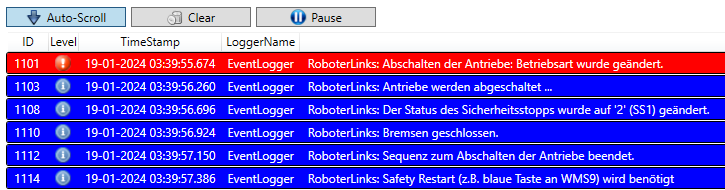
\includegraphics[width=1\linewidth]{./images/Fehlermeldung.png}
   		\caption{Anzeige Systemereignisse}
   		\label{fig:AnzeigeEvents}
   	\end{figure}\\
   	\textbf{2. Übertragung bei Umteachen}\\
   	Ebenso wurde beim Umteachen von Bewegungspunkten erfolgreich eine Meldung in der WPF-Anwendung ausgegeben (vgl. Abbildung \ref{fig:Umteachen}).
   	\begin{figure}[!ht]
   		\centering
   		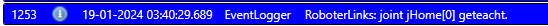
\includegraphics[width=1\linewidth]{./images/Umteachen.png}
   		\caption{Meldung bei Umteachen von Bewegungspunkten}
   		\label{fig:Umteachen}
   	\end{figure}\\
   	\textbf{3. Änderung Ereignisschwere}\\
   	Nach Anpassung der Ereigniss-Schwere in der WPF-Anwendung wurden wie gewünscht nur noch die Systemereignisse aber dieser Schwere übertragen. Bei Setzten der Ereignis-Schwere auf 2 wurden die einfachen Informationsmeldungen nicht mehr übertragen, sondern lediglich Warnungen oder noch schwerwiegendere Ereignisse.\\
   	\textbf{4. Anzeige der Prozessdaten}\\
   	Die Prozessdaten des Roboters werden wie gewünscht in der WPF-Anwendung angezeigt (vgl. Abbildung \ref{fig:Prozessdaten}). Ebenso ist es möglich zwischen potentiell mehreren Robotern über ein Drop-Down-Menü zu wechseln. Über die Aktualisierungs-Schaltfläche können die Grafiken aktualisiert werden.
   	\begin{figure}[!ht]
   		\centering
   		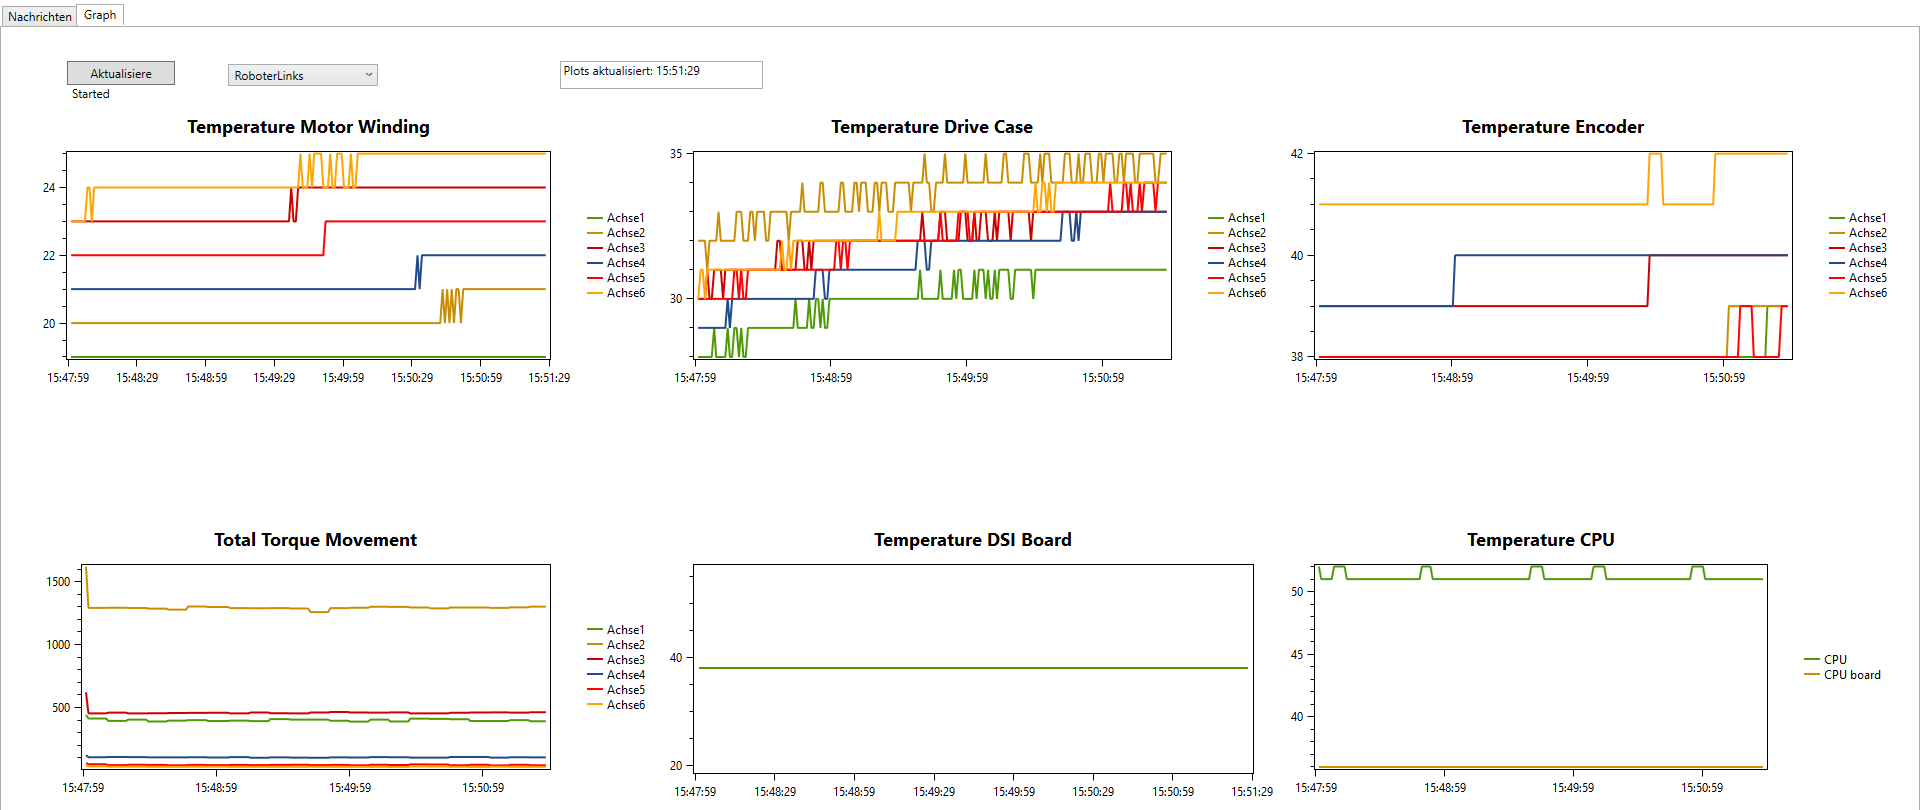
\includegraphics[width=1\linewidth]{./images/Prozessdaten.png}
   		\caption{Visualisierung der Prozessdaten}
   		\label{fig:Prozessdaten}
   	\end{figure}\\
   	\textbf{5. Integration der Motormomente}\\
   	Eine Besonderheit stellen die Motormomente dar, da diese nicht wie andere Prozessdaten unverarbeitet übertragen werden, sondern über einen gesamten Bewegungsablauf über die Zeit integriert werden. Im Testfall wurde auf den Greifer zeitweise eine externe Kraft aufgebracht, um den Einfluss der Last auf das Motormoment zu erkennen. In dem Drehmomentenverlauf ist ein deutlicher Anstieg der Momente, in den Bewegungsabläufen zu sehen, in denen eine Kraft aufgeprägt war (vgl. Abbildung \ref{fig:Motormomente}). Für die Motormomente, ergeben sich vielfältige Nutzungspotentiale. Ein Anstieg der Motormomente kann darauf hindeuten, dass die Achse geschmiert werden soll oder das ein Defekt z.B. am Lager vorliegt. Bei Überschreiten von Grenzwerten, die für jeden Anwendungsfall individuell bestimmt werden müssen, kann der Bediener gewarnt werden. Im Idealfall kann bereits durch das Erkennen von Tendenzen im Momentenverlauf, eine Wartung vorgenommen werden, bevor eine Schädigung überhaupt eintritt. Hierbei spricht man von vorausschauender Wartung, was die Ausfallzeiten der Anlage deutlich reduzieren kann.
   	\begin{figure}[!ht]
   		\centering
   		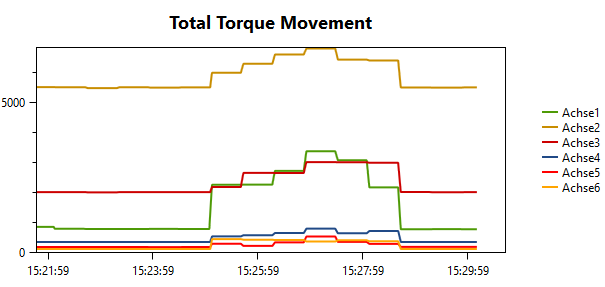
\includegraphics[width=0.7\linewidth]{./images/Motormomente.png}
   		\caption{Visualisierung der integrierten Motormomente}
   		\label{fig:Motormomente}
   	\end{figure}\\
   	\textbf{6. Binäre Werte zur Fehlerüberwachung}\\
   	Von dem Roboter werden eine Vielzahl an binären Werten zu der WPF-Anwendung übertragen. Manche von ihnen sind ein Fehlerindikator. Wird z.B. der CPU Überstrom auf true bei dem Roboter manipuliert, wird dies von der WPF-Anwendung in der Fehleranalyse wie gewünscht entdeckt und ausgegeben (vgl. Abbildung \ref{fig:binarFehler}).
   	\begin{figure}[!ht]
   		\centering
   		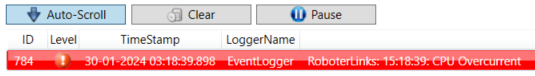
\includegraphics[width=0.7\linewidth]{./images/BinarFehler.png}
   		\caption{Binäre Werte zur Fehlerüberwachung}
   		\label{fig:binarFehler}
   	\end{figure}\\
   	\textbf{7. Verbindung mehrerer Roboter}\\
   	Durch eine virtuelle Client-Anwendung wird der Einsatz von mehreren Robotern nachgebildet. Die Kommunikation der WPF-Anwendung mit mehreren Clients erfolgt wie gewünscht und es erfolgt eine Ausgabe der verbundenen Clients (Roboter) im dafür eingerichteten Ausgabefelder der WPF-Anwendung (vgl. Abbildung \ref{fig:VerbundeneRoboter}).
   	\begin{figure}[!ht]
   		\centering
   		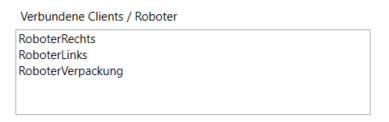
\includegraphics[width=0.7\linewidth]{./images/VerbundeneRoboter.png}
   		\caption{Anzeige der verbundenen Roboter}
   		\label{fig:VerbundeneRoboter}
   	\end{figure}\\
   	\section{Fehlertests}
   	Ein Fehler ist dadurch definiert, dass das Ergebnis nicht den Anforderungen entspricht und es zu einem Fehlverhalten kommt. \cite{pilorget2012test}\\
   	Fehler können sehr vielfältiger Natur sein. Insbesondere solche, die nur in speziellen Ausnahmefällen auftreten, sind schwer zu entdecken. Ein Ermitteln und Testen aller Ausnahmefällen ist daher schlicht unmöglich. Ziel ist es daher, möglichst viele spezielle Anforderungen an das System zu identifizieren, welche zu Fehlern führen können und diese anschließend zu testen. Für eine systematische Analyse von potentiellen Fehlerursachen sollen ein Fehlerbäume eingesetzt werden. Diese ermöglichen es Zusammenhänge zwischen Ursache und Wirkung darzustellen. \cite{liggesmeyer2009software}\\
   	Hierzu werden in einem ersten Schritt mögliche Fehler, wie z.B. ein Programm-Absturz durch Brainstorming identifiziert. In einem zweiten Schritt werden mögliche Ursachen ermittelt, welche zu den genannten Fehlern führen könnten. Ein Testen durch bewusste Provozieren dieser Fehlerursachen ermöglicht es potentielle Fehler zu entdecken und die Fehlertoleranz des Systems zu validieren. Die entworfenen Fehlerbäume für mögliche Fehler sind nachfolgend dargestellt (vgl. Abbildung \ref{fig:Fehlerbaum_1}, \ref{fig:Fehlerbaum_2}, \ref{fig:Fehlerbaum_3} und \ref{fig:Fehlerbaum_4}).

   	
   	\begin{figure}[h!]
   		\centering
   		\begin{forest}
   			for tree={
   				parent anchor=south,
   				child anchor=north,
   				l sep+=1mm,
   				s sep+=1mm, % kleinerer vertikaler Abstand
   				if n children={0}{
   					tier=terminus,
   					draw,
   					rectangle,
   					rounded corners,
   					fill=red!20,
   				}{},
   			}
   			[Verbindungsabbruch
   			[\fbox{$\geq 1$}
   			[Entferntes LAN-Kabel
   			]
   			[Neustart Anlagenvisualierung
   			]
   			[Neustart Roboter
   			]
   			]
   			]
   		\end{forest}
   		\caption{Fehlerbaumdiagramm Verbindungsabbruch}
   		\label{fig:Fehlerbaum_1}
   	\end{figure}
   	
   	\begin{figure}[h!]
   		\centering
   		\begin{forest}
   			for tree={
   				parent anchor=south,
   				child anchor=north,
   				l sep+=0.5mm,
   				s sep+=1mm, % kleinerer vertikaler Abstand
   				if n children={0}{
   					tier=terminus,
   					draw,
   					rectangle,
   					rounded corners,
   					fill=red!20,
   				}{},
   			}
   			[Nachrichtenverzug
   			[\fbox{$\geq 1$}
   			[Viele Systemereignisse
   			]
   			[Hohe Datenanforderungsrate
   			]
   			]
   			]
   		\end{forest}
   		\caption{Fehlerbaumdiagramm Nachrichtenverzug}
   		\label{fig:Fehlerbaum_2}
   	\end{figure}
   	
   	\begin{figure}[h!]
   		\centering
   		\begin{forest}
   			for tree={
   				parent anchor=south,
   				child anchor=north,
   				l sep+=0.5mm,
   				s sep+=1mm, % kleinerer vertikaler Abstand
   				if n children={0}{
   					tier=terminus,
   					draw,
   					rectangle,
   					rounded corners,
   					fill=red!20,
   				}{},
   			}
   			[Absturz Roboterprogramm
   			[\fbox{$\geq 1$}
   			[Entferntes LAN-Kabel
   			]
   			[Neustart Anlagenvisualisierung
   			]
   			]
   			]
   		\end{forest}
   		\caption{Fehlerbaumdiagramm Absturz Roboterprogramm}
   		\label{fig:Fehlerbaum_3}
   	\end{figure}
   	
   	\begin{figure}[h!]
   		\centering
   		\begin{forest}
   			for tree={
   				parent anchor=south,
   				child anchor=north,
   				l sep+=0.5mm,
   				s sep+=1mm, % kleinerer vertikaler Abstand
   				if n children={0}{
   					tier=terminus,
   					draw,
   					rectangle,
   					rounded corners,
   					fill=red!20,
   				}{},
   			}
   			[Absturz WPF-Anwendung
   			[\fbox{$\geq 1$}
   			[\begin{tabular}{@{}c@{}}Entferntes \\ LAN-Kabel\end{tabular}
   			]
   			[\begin{tabular}{@{}c@{}}Neustart \\ Roboter\end{tabular}
   			]
   			[\begin{tabular}{@{}c@{}}Erhalt falscher \\ Nachricht\end{tabular}
   			]
   			[\begin{tabular}{@{}c@{}}CSV-Datei \\ gesperrt/gelöscht\end{tabular}
   			]
   			]
   			]
   		\end{forest}
   		\caption{Fehlerbaumdiagramm Absturz WPF-Anwendung}
   		\label{fig:Fehlerbaum_4}
   	\end{figure}
   	\noindent
   	Alle ermittelten möglichen Fehlerursachen, wie z.B. das Entfernen des LAN-Kabels, wurden zur Validierung getestet, um auszuschließen, dass es zu einem Fehler kommt.
   	Nach kleineren Optimierungen an der WPF-Anwendung ist es dem System nun möglich, auf alle potentiellen Fehlerursachen zu reagieren und eine robuste und fehlerfreie Fortführung des Systems zu gewährleisten. Beispielsweise wird beim Neustart des Roboters eine Meldung in der WPF-Anwendung ausgegeben, dass die Verbindung verloren gegangen ist. Nach dem Wiederhochfahren baut die Verbindung jedoch selbst wieder auf und die Kommunikation fährt automatisch fort. Ebenso verursacht ein Löschen der CSV-Datei keinen Fehler, da in diesem Fall das System selbst eine neue Datei anlegt. Wird die CSV-Datei durch ein anderes System, wie z.B. Excel blockiert, hindert dies die Funktionsweise nicht, da sich die WPF-Anwendung eine Kopie der CSV-Datei anlegt. Eine Validierung des Systems ist hiermit nach bestem Gewissen sichergestellt. Dennoch ist darauf hinzuweisen, dass besondere unvorhergesehene Ereignisse nicht ausgeschlossen werden können. Die Robustheit von Software kann jedoch durch längerfristige Benutzung im Betrieb weiter verbessert werden. 

   	\chapter{Ausblick und Fazit}
   	Übertrag auf andere Hersteller
   	\backmatter
   	
   	
   	\cleardoublepage
   	\listoffigures
   	\cleardoublepage
   	\listoftables
   	\cleardoublepage
   	
   	\cleardoublepage
   	\printbibliography
   	
   	% Acronyms   	
   	% Appendix, if needed:
   

\end{document}